\documentclass[
	% -- opções da classe memoir --
	12pt,				% tamanho da fonte
	openright,			% capítulos começam em pág ímpar (insere página vazia caso preciso)
	oneside,			% para impressão em verso e anverso. Oposto a oneside
	a4paper,			% tamanho do papel. 
	% -- opções da classe abntex2 --
	%chapter=TITLE,		% títulos de capítulos convertidos em letras maiúsculas
	%section=TITLE,		% títulos de seções convertidos em letras maiúsculas
	%subsection=TITLE,	% títulos de subseções convertidos em letras maiúsculas
	%subsubsection=TITLE,% títulos de subsubseções convertidos em letras maiúsculas
	% -- opções do pacote babel --
	english,			% idioma adicional para hifenização
	brazil,				% o último idioma é o principal do documento
    fleqn,
	]{abntex2}


% ---
% PACOTES
% ---

% ---
% Pacotes fundamentais 
% ---
\usepackage[T1]{fontenc}		% Selecao de codigos de fonte.
\usepackage[portuguese,portuguesekw,linesnumbered,ruled,lined,commentsnumbered]{algorithm2e}
\usepackage{algorithmic}
\usepackage{enumitem}
\usepackage{subcaption}
\usepackage[utf8]{inputenc}		% Codificacao do documento (conversão automática dos acentos)
\usepackage{lastpage}			% Usado pela Ficha catalográfica
\usepackage{indentfirst}		% Indenta o primeiro parágrafo de cada seção.
\usepackage{color}				% Controle das cores
\usepackage{graphicx}			% Inclusão de gráficos


\usepackage{multirow}
\usepackage{array}
\usepackage[table,xcdraw]{xcolor}
\usepackage{longtable}
\usepackage{amssymb}
\usepackage{amsmath}
\usepackage{mathtools}
\usepackage{nccmath}
\usepackage{multicol}
\usepackage{booktabs}
\usepackage{subcaption}
\usepackage{hyperref}
\usepackage{tikz}
\usetikzlibrary{shapes.geometric, arrows.meta, positioning, fit, calc}
\usepackage{listings}
\usepackage{setspace}
\usepackage{makecell}
\usepackage{pdfpages}

\definecolor{codegreen}{rgb}{0,0.6,0}
\definecolor{codegray}{rgb}{0.5,0.5,0.5}
\definecolor{codepurple}{rgb}{0.58,0,0.82}
\definecolor{backcolour}{rgb}{0.95,0.95,0.92}

\lstdefinestyle{mystyle}{
    backgroundcolor=\color{backcolour},   
    commentstyle=\color{codegreen},
    keywordstyle=\color{magenta},
    numberstyle=\tiny\color{codegray},
    stringstyle=\color{codepurple},
    basicstyle=\ttfamily\footnotesize,
    breakatwhitespace=false,         
    breaklines=true,                 
    captionpos=b,                    
    keepspaces=true,                 
    numbers=left,                    
    numbersep=5pt,                  
    showspaces=false,                
    showstringspaces=false,
    showtabs=false,                  
    tabsize=2
}

\lstset{style=mystyle}

% Tabela
\renewcommand{\arraystretch}{1.2}
% ---
		
% ---
% Pacotes adicionais, usados apenas no âmbito do Modelo Canônico do abnteX2
% ---
\usepackage{lipsum}				% para geração de dummy text
% ---

% ---
% Pacotes de citações
% ---
\usepackage[brazilian,hyperpageref]{backref}	 % Paginas com as citações na bibl
\usepackage[alf]{abntex2cite}	% Citações padrão ABNT
\usepackage{lscape}

\usepackage{pdfpages}
\usepackage{amsmath}



%% Novo estilo
\makepagestyle{estilo_pretextual} %%% escolha um nome
  \makeevenhead{estilo_pretextual}{}{}{\ABNTEXfontereduzida \textbf \thepage}
  \makeoddhead{estilo_pretextual}{}{}{\ABNTEXfontereduzida \textbf \thepage}

%% Customiza comando \pretextual
\renewcommand{\pretextual}{
  \pagenumbering{roman} %%% ou \pagenumbering{Roman}
  \aliaspagestyle{chapter}{estilo_pretextual}% customizing chapter pagestyle
  \pagestyle{estilo_pretextual}
  \aliaspagestyle{cleared}{empty}
  \aliaspagestyle{part}{estilo_pretextual}
}

% ---
% Ajusta a marca \textual para que a numeração volte a ser arábica
% nos elementos textuais
\let\oldtextual\textual        % copia o comando \textual anterior para \oldtextual
\newcounter{start}	%Contador para começar arábico considerando numeração romana
\renewcommand{\textual}{%
  \oldtextual%
  \setcounter{start}{\value{page}}
  \pagenumbering{arabic} % volta à numeração arábica
  \setcounter{page}{\thestart{}}
}
% ---



% --- 
% CONFIGURAÇÕES DE PACOTES
% --- 

% ---
% Configurações do pacote backref
% Usado sem a opção hyperpageref de backref
\renewcommand{\backrefpagesname}{Citado na(s) página(s):~}
% Texto padrão antes do número das páginas
\renewcommand{\backref}{}
% Define os textos da citação
\renewcommand*{\backrefalt}[4]{
	\ifcase #1 %
		Nenhuma citação no texto.%
	\or
		Citado na página #2.%
	\else
		Citado #1 vezes nas páginas #2.%
	\fi}%
% ---

\usepackage[colorinlistoftodos,prependcaption,textsize=tiny]{todonotes}
\usepackage{soul} 
\newcommand{\alterar}[2][]{\todo[linecolor=black,backgroundcolor=orange!25,bordercolor=red,#1]{\textbf{Alterar}: #2}}
\newcommand{\adicionadomarcelo}[1]{#1}
\newcommand{\removido}[1]{#1}

\newcommand{\mantido}[1]{#1}
\newcommand{\modificado}[1]{#1}

\newcommand{\dica}[2][]{\todo[linecolor=blue,backgroundcolor=blue!25,bordercolor=blue,#1]{\textbf{Dica}: #2}}

\newcommand{\comentmargin}[2][]{\todo[linecolor=blue,backgroundcolor=green!25,bordercolor=green,#1]{#2}}
\newcommand{\comentline}[2][]{\todo[inline, linecolor=yellow,backgroundcolor=green!25,bordercolor=green,#1]{\textbf{Comentário}: #2}}

\newenvironment{BlocoRevisadoSemAlteracao}
{
	\color{blue}%
}
{
}

\newenvironment{BlocoRevisadoEsperandoAlteracao}
{
	\color{orange}%
}
{
}

\makeatother
% --- 

% --- 
% Espaçamentos entre linhas e parágrafos 
% --- 

% O tamanho do parágrafo é dado por:
\setlength{\parindent}{1.5cm}

% Controle do espaçamento entre um parágrafo e outro:
\setlength{\parskip}{0.2cm}  % tente também \onelineskip

% ---
% compila o indice
% ---
\makeindex
% ---

% ----
% Início do documento
% ----
\allowdisplaybreaks


\DeclareCaptionType{code}[Código][Lista de Códigos] 

\begin{document}


%% ---
% Informações de dados para CAPA e FOLHA DE ROSTO
% ---
\titulo{[TO DO] Seu Título}
\autor{[TO DO] Nome Completo}
\local{Diamantina/MG}
\data{2023}
\orientador{Prof. Dr. Marcelo Ferreira Rego}
%\coorientador{Equipe \abnTeX}
\instituicao{%
  UNIVERSIDADE FEDERAL DOS VALES DO JEQUITINHONHA E MUCURI
  \par
  Bacharelado em Sistemas de Informação 
  }
\tipotrabalho{Monografia (Graduação)}

% O preambulo deve conter o tipo do trabalho, o objetivo, 
% o nome da instituição e a área de concentração 
\preambulo{Monografia apresentada ao Curso de Sistemas de Informação do Departamento de Computação da Universidade Federal dos Vales do Jequitinhonha e Mucuri como requisito parcial para obtenção do título de Bacharel em Sistemas de Informação.}
% ---


\pretextual

% ---
% Capa (Obrigatório)
% ---
\imprimircapa
% ---

% ---
% Folha de rosto (obrigatório)
% (o * indica que haverá a ficha bibliográfica)
% ---
\imprimirfolhaderosto
% ---


% ---
% Inserir a ficha bibliografica
% ---

% Isto é um exemplo de Ficha Catalográfica, ou ``Dados internacionais de
% catalogação-na-publicação''. Você pode utilizar este modelo como referência. 
% Porém, provavelmente a biblioteca da sua universidade lhe fornecerá um PDF
% com a ficha catalográfica definitiva após a defesa do trabalho. Quando estiver
% com o documento, salve-o como PDF no diretório do seu projeto e substitua todo
% o conteúdo de implementação deste arquivo pelo comando abaixo:
%
% \begin{fichacatalografica}
%     \includepdf{fig_ficha_catalografica.pdf}
% \end{fichacatalografica}
\begin{comment}
\begin{fichacatalografica}
	\vspace*{\fill}					% Posição vertical
	\hrule							% Linha horizontal
	\begin{center}					% Minipage Centralizado
	\begin{minipage}[c]{12.5cm}		% Largura
	
	\imprimirautor
	
	\hspace{0.5cm} \imprimirtitulo  / \imprimirautor. --
	\imprimirlocal, \imprimirdata-
	
	\hspace{0.5cm} \pageref{LastPage} p. : il. (algumas color.) ; 30 cm.\\
	
	\hspace{0.5cm} \imprimirorientadorRotulo~\imprimirorientador\\
	
	\hspace{0.5cm}
	\parbox[t]{\textwidth}{\imprimirtipotrabalho~--~\imprimirinstituicao,
	\imprimirdata.}\\
	
	\hspace{0.5cm}
		1. Palavra-chave1.
		2. Palavra-chave2.
		I. Orientador.
		II. Universidade xxx.
		III. Faculdade de xxx.
		IV. Título\\ 			
	
	\hspace{8.75cm} CDU 02:141:005.7\\
	
	\end{minipage}
	\end{center}
	\hrule
\end{fichacatalografica}
\end{comment}
% ---


% ---
% Inserir Errata (opcional)
% ---
\begin{comment}
\begin{errata}
Elemento opcional da \citeonline[4.2.1.2]{NBR14724:2011}. Exemplo:

\vspace{\onelineskip}

FERRIGNO, C. R. A. \textbf{Tratamento de neoplasias ósseas apendiculares com
reimplantação de enxerto ósseo autólogo autoclavado associado ao plasma
rico em plaquetas}: estudo crítico na cirurgia de preservação de membro em
cães. 2011. 128 f. Tese (Livre-Docência) - Faculdade de Medicina Veterinária e
Zootecnia, Universidade de São Paulo, São Paulo, 2011.

\begin{table}[htb]
\center
\footnotesize
\begin{tabular}{|p{1.4cm}|p{1cm}|p{3cm}|p{3cm}|}
  \hline
   \textbf{Folha} & \textbf{Linha}  & \textbf{Onde se lê}  & \textbf{Leia-se}  \\
    \hline
    1 & 10 & auto-conclavo & autoconclavo\\
   \hline
\end{tabular}
\end{table}

\end{errata}
\end{comment}
% ---

% ---
% Inserir Folha de aprovação (obrigatório)
% ---

% Isto é um exemplo de Folha de aprovação, elemento obrigatório da NBR
% 14724/2011 (seção 4.2.1.3). Você pode utilizar este modelo até a aprovação
% do trabalho. Após isso, substitua todo o conteúdo deste arquivo por uma
% imagem da página assinada pela banca com o comando abaixo:
%
%\includepdf[pages=-]{folhadeaprovacao.pdf}
%

%TODO Adicionar folha de aprovação
\begin{folhadeaprovacao}

\includepdf[scale=0.9, pages=1-2, pagecommand={}]{folhadeaprovacao.pdf}
  
\end{folhadeaprovacao}
% ---

% ---
% Dedicatória (opcional)
% ---
% \begin{dedicatoria}
%    \vspace*{\fill}
%    \centering
%    \noindent
%    \textit{Dedico este trabalho à minha família...} \vspace*{\fill}
% \end{dedicatoria}
% ---

% ---
% Agradecimentos (opcional)
% ---
\begin{agradecimentos}

%TODO
[TO DO] Escreva seu agradecimento

\end{agradecimentos}
% ---

% ---
% Epígrafe (opcional)
% ---
\begin{epigrafe}
    \vspace*{\fill}
	\begin{flushright}
		\textit{"A persistência é o caminho do êxito." (Charles Chaplin)}
	\end{flushright}
\end{epigrafe}
% ---

% ---
% RESUMOS
% ---

% resumo em português
% Resumo em língua vernácula (obrigatório)
\begin{resumo}
% TODO: escrever resumo do TCC (150-300 palavras) cobrindo: contexto, problema, objetivo, metodologia, resultados (quando houver), conclusao.

\vspace{\onelineskip}
\noindent
\textbf{Palavras-chaves}: poda neural; eficiência energética; compressão de modelo de IA; otimização estrutural de redes neurais.
\end{resumo}

% resumo em inglês
% Resumo em língua estrangeira (obrigatório)
\begin{resumo}[\textbf{Abstract}]
 \begin{otherlanguage*}{english}

[TO DO] Abstract em um parágrafo.
    
   \vspace{\onelineskip}
 
   \noindent 
   \textbf{Key-words}: [TO DO] Key-words separadas por ponto-e-vírgula
 \end{otherlanguage*}
\end{resumo}
% ---

% ---
% inserir lista de ilustrações  essa lista é prenchida automatica  com as imagens inseridas no documento
% Listas de ilustrações (opcional)
% ---
\pdfbookmark[0]{\listfigurename}{lof}
\listoffigures*
\cleardoublepage
% ---

% ---
% inserir lista de tabelas é prenchida automatica  com as tabelas  inseridas no documento
% Lista de tabelas (opcional)
% ---
\pdfbookmark[0]{\listtablename}{lot}
\listoftables*
\cleardoublepage
% ---

% ---
% inserir lista de abreviaturas e siglas inserir caso houver
% Lista de abreviaturas (opcional)
% Lista de siglas (opcional)
% ---
\begin{siglas}
    \item [TO DO] {\em [TO DO]}
 \end{siglas}
% ---


% ---
% inserir lista de símbolos
% Lista de símbolos (opcional)
% ---
\begin{comment}
\begin{simbolos}
  \item[$ \Gamma $] Letra grega Gama
  \item[$ \Lambda $] Lambda
  \item[$ \zeta $] Letra grega minúscula zeta
  \item[$ \in $] Pertence
\end{simbolos}
\end{comment}
% ---

% ---
% inserir lista de algoritmos lista os algoritimos automatico
% Lista de algoritmos (opcional)
% ---
\pdfbookmark[0]{\listtablename}{loa}
\listofcodes
\cleardoublepage
% ---


% ---
% inserir o sumario é preenchido automatico de acordo que é criado no documento
% Sumário (obrigatório)
% ---
\pdfbookmark[0]{\contentsname}{toc}
\textbf{\tableofcontents*}
\cleardoublepage
% ---

\textual

%\setcounter{page}{7}


\chapter{Introdução}\label{capitulo1}

[TODO] 



\section{Objetivos}

[TODO]

\subsection{Objetivo Geral}

[TODO]

\subsection{Objetivos Específicos}
    [TODO]

\section{Organização da monografia}

[TODO]

Este trabalho é composto por XX capítulos. Neste Capítulo \ref{capitulo1}, proporcionamos uma introdução, justificativa e delineamos os objetivos...
% =============================================================
% Capítulo 2 — Fundamentação Teórica
% =============================================================

\chapter{Fundamentação Teórica}\label{chap:fundamentacao_teorica}

\adicionadomarcelo{Este capítulo apresenta os conceitos necessários para a compreensão do trabalho. Inicialmente, são introduzidos fundamentos de aprendizado profundo e redes neurais artificiais, seguidos pelo processo de treinamento dessas redes. Em seguida, discute-se o problema do consumo energético em modelos de \textit{Deep Learning} e, por fim, são apresentadas as técnicas de compressão de modelos, com destaque para a poda neural (\textit{pruning}), que é o foco deste trabalho.}

A exposição é deliberadamente progressiva e não pressupõe familiaridade prévia com
aprendizado de máquina. Cada conceito é introduzido primeiro por meio de uma analogia com
situações cotidianas e só então formalizado, de modo que o leitor possa acompanhar o
raciocínio antes de encontrar a notação matemática que o descreve.

\section{Aprendizado Profundo e Redes Neurais}

\subsection{Aprendizado Profundo (Deep Learning)}
O Aprendizado Profundo é um campo especializado de aprendizado de máquina \adicionadomarcelo{\cite{Goodfellow2016,LeCun2015}}, \modificado{caracterizado pelo uso de redes neurais artificiais com múltiplas camadas, o que permite aprender e extrair informações complexas a partir de grandes volumes de dados}.

\subsection{Redes Neurais Artificiais}
\modificado{A rede neural artificial é um modelo computacional inspirado na estrutura do cérebro humano, que busca imitar a forma como neurônios se conectam e processam sinais para aprender a partir de dados, identificando padrões e tomando decisões. Um exemplo clássico é o perceptron multicamadas (MLP), um modelo composto por funções matemáticas que mapeiam valores de entrada em valores de saída \cite{Goodfellow2016}. Em tarefas de visão computacional, por exemplo, milhões de imagens de um objeto podem ser processadas para que a rede aprenda suas características visuais e seja capaz de reconhecê-lo posteriormente.}

Uma forma de tentar enteder a definição de uma RNN é, imagine uma comissão
encarregada de decidir se um pedido de empréstimo deve ser aprovado. Nenhum membro decide
sozinho, cada um examina um aspecto diferentee, como a renda declarada, o histórico de
pagamentos, o tempo de emprego e então, após analisar todos os aspectos, emite um parecer. Esses pareceres não têm todos o
mesmo valor, pois a comissão confia mais em uns avaliadores do que em outros, e a decisão
final combina todos eles, ponderados por essa confiança. Em uma rede neural, cada nó é um
desses avaliadores e o peso de cada conexão é exatamente a confiança depositada naquele
parecer. A diferença essencial é que a rede não recebe essas confianças prontas, ela as
descobre sozinha, por tentativa e erro, ao longo do treinamento.

Uma rede neural profunda é composta por unidades (nós) interconectadas, organizadas em camadas
\cite{Goodfellow2016,NielsenNNDL2015}.

\begin{itemize}
    \item \textbf{Nó (neurônio):} É uma unidade computacional que calcula uma soma ponderada das entradas mais um \textit{bias} e passa o resultado através de uma função de ativação, produzindo uma saída.
    \item \textbf{Camada de Entrada (Input Layer):} É onde o processo é iniciado e os dados são introduzidos na rede. O número de nós nessa camada corresponde ao número de características dos dados de entrada.
    \item \textbf{Camadas Ocultas (Hidden Layers):} São camadas intermediárias entre a entrada e a saída. Cada nó de uma camada oculta está conectado a todos os nós das camadas anterior e seguinte. É nelas que ocorre a maior parte do processamento e do aprendizado; a saída de uma camada oculta é utilizada como entrada da próxima, e, a cada camada, a rede passa a detectar características mais complexas e abstratas. Redes com múltiplas camadas ocultas são as chamadas redes de \textit{Deep Learning}.
    \item \textbf{Camada de Saída (Output Layer):} Camada final da rede, onde o resultado é produzido. A estrutura da camada de saída depende da tarefa: em regressão, há um único nó com função de ativação linear; em classificação binária, um único nó expressa resultados do tipo sim/não; em classificação multiclasse, há um nó para cada classe possível, e o de maior ativação corresponde à predição final.
\end{itemize}

\modificado{Cada conexão entre nós possui um peso associado, que determina a sua importância relativa. Pesos altos amplificam o sinal de entrada, enquanto pesos próximos de zero tornam a conexão pouco influente. Os pesos são inicializados com valores aleatórios e ajustados durante o treinamento \cite{Goodfellow2016}.}

% \begin{figure}[htb]
% \centering
% \caption{\adicionadomarcelo{Arquitetura típica de uma rede neural artificial com uma camada de entrada, duas camadas ocultas e uma camada de saída.}}
% \label{fig:arquitetura_rede_neural}
% 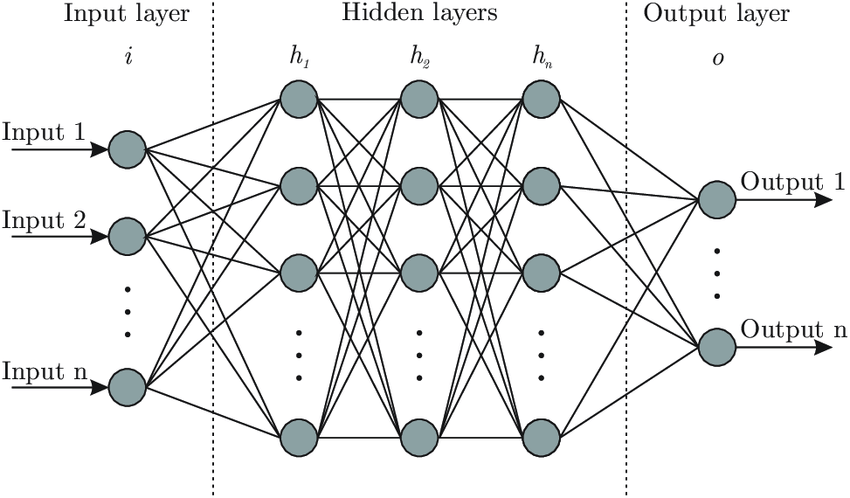
\includegraphics[scale=0.45]{02_capitulo/imageArquiteturaRedeNeural.png}
% % \\ \adicionadomarcelo{Fonte: \citeonline{NielsenNNDL2015}.}
% \end{figure}

\subsection{Bias em Redes Neurais}
\modificado{O \textit{bias} é um parâmetro adicional que ajusta a saída de um neurônio. Trata-se de um valor numérico associado a cada neurônio, não ligado a nenhuma entrada específica, atuando como um coeficiente linear. Antes da aplicação da função de ativação, o \textit{bias} é somado ao resultado da soma ponderada das entradas.}

A principal função do \textit{bias} é deslocar a função de ativação, permitindo que o modelo se ajuste melhor aos dados. Sem ele, a soma ponderada precisaria ser alta para que o neurônio fosse ativado; com o \textit{bias}, um neurônio pode ser ativado mesmo com uma soma ponderada baixa, caso seu \textit{bias} seja suficientemente alto \cite{NielsenNNDL2015}. Inversamente, um \textit{bias} muito negativo dificulta a ativação do neurônio. \modificado{O \textit{bias} é um parâmetro aprendível: inicialmente é inicializado com zero ou valores próximos de zero e, durante o treinamento, é atualizado pelo mesmo processo de retropropagação e descida de gradiente utilizado para os pesos.}

Retomando com a analogia da comissão de crédito, se os pesos representam o quanto se confia em cada
avaliador, o \textit{bias} representa o quanto o avaliador é exigente. Um membro
gentil aprova o pedido mesmo diante de evidências modestas; um membro rigoroso só
aprova quando as evidências são fortes. São duas coisas independentes --- confiar muito em
alguém não diz nada sobre o quanto essa pessoa é exigente --- e é por isso que a rede
precisa aprender os dois conjuntos de valores separadamente.

\subsection{Função de Ativação}
\modificado{A função de ativação é uma função matemática aplicada ao resultado da soma ponderada das entradas de um neurônio (já acrescido do \textit{bias}), determinando a saída do neurônio. Sua principal função é introduzir não linearidade no modelo: sem ela, a composição de diversas camadas resultaria em uma transformação puramente linear, equivalente a uma rede com uma única camada, o que limitaria drasticamente a capacidade expressiva do modelo \cite{Goodfellow2016}.}

A razão de existir dessa função merece um exemplo concreto, pois é ela que justifica o
próprio empilhamento de camadas. Considere um produto de R\$ 100,00 submetido a dois
descontos sucessivos, um de 10\% e outro de 20\%: o primeiro leva o preço a R\$ 90,00 e o
segundo a R\$ 72,00, exatamente o mesmo resultado que um único desconto de 28\% produziria.
Os dois passos colapsaram em um só, e o segundo nada acrescentou que um único desconto bem
escolhido não fizesse sozinho. Encadear operações lineares nunca gera nada além de outra
operação linear, e com redes neurais acontece o mesmo: sem função de ativação, uma rede de
cem camadas calcularia exatamente aquilo que uma única camada já calcularia, e toda a
profundidade seria desperdiçada.

Suponha agora que a loja adote uma regra adicional, aplicada logo depois de cada desconto:
nenhum produto pode ser vendido por menos de R\$ 85,00. Essa regra é o análogo da função de
ativação --- ela não faz parte do desconto, mas incide sobre o resultado dele, antes que
esse resultado siga para a etapa seguinte. Com ela, o encadeamento deixa de colapsar. O
produto de R\$ 100,00 cai para R\$ 90,00 e depois para R\$ 72,00, mas a regra o devolve a
R\$ 85,00, de modo que o desconto efetivo foi de 15\%. Já um produto de R\$ 200,00 percorre
os mesmos dois descontos, chega a R\$ 144,00 sem nunca esbarrar no limite e tem desconto
efetivo de 28\%. A mesma sequência de operações passou a produzir resultados diferentes
conforme a entrada, e nenhum desconto único reproduz esse comportamento. É esse
rompimento do encadeamento que permite a cada camada acrescentar algo que a anterior não
conseguia representar. A regra de preço mínimo, aliás, tem a mesma forma da ReLU,
apresentada adiante nesta seção: ambas preservam os valores acima de um limiar e
substituem os demais por um valor fixo.

A ativação de um neurônio ocorre em três etapas \cite{NielsenNNDL2015}:
\begin{itemize}
    \item \modificado{Soma ponderada: o neurônio multiplica o valor de ativação de cada nó da camada anterior pelo peso da respectiva conexão e soma todos os resultados.}
    \item \modificado{Adição do \textit{bias}: ao resultado da soma ponderada é somado o valor do \textit{bias}, que auxilia o neurônio a ativar-se mais ou menos facilidade.}
    \item \modificado{Função de ativação: o resultado final (soma ponderada acrescida do \textit{bias}) é passado pela função de ativação, cuja saída é então transmitida aos nós da próxima camada.}
\end{itemize}

\begin{figure}[htb]
\centering
\caption{\adicionadomarcelo{Representação matricial da propagação de um neurônio, da soma ponderada à função de ativação (Sigmoide).}}
\label{fig:matrizes_sigmoid}
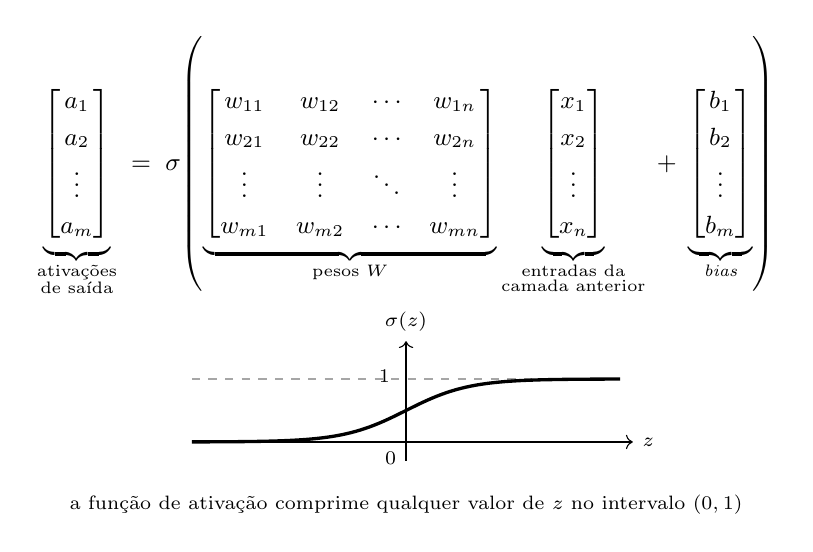
\begin{tikzpicture}[font=\small]
  \node at (0,0) {$
    \underbrace{\begin{bmatrix} a_1 \\ a_2 \\ \vdots \\ a_m \end{bmatrix}}_{\substack{\text{ativações}\\\text{de saída}}}
    \;=\; \sigma\!\left(
    \underbrace{\begin{bmatrix}
      w_{11} & w_{12} & \cdots & w_{1n} \\
      w_{21} & w_{22} & \cdots & w_{2n} \\
      \vdots & \vdots & \ddots & \vdots \\
      w_{m1} & w_{m2} & \cdots & w_{mn}
    \end{bmatrix}}_{\text{pesos } W}
    \underbrace{\begin{bmatrix} x_1 \\ x_2 \\ \vdots \\ x_n \end{bmatrix}}_{\substack{\text{entradas da}\\\text{camada anterior}}}
    \;+\;
    \underbrace{\begin{bmatrix} b_1 \\ b_2 \\ \vdots \\ b_m \end{bmatrix}}_{\textit{bias}}
    \right)$};
  \begin{scope}[shift={(0,-3.5)}, scale=0.8]
    \draw[->] (-3.4,0) -- (3.6,0) node[right,font=\scriptsize] {$z$};
    \draw[->] (0,-0.3) -- (0,1.6) node[above,font=\scriptsize] {$\sigma(z)$};
    \draw[dashed,gray!70] (-3.4,1) -- (3.4,1);
    \node[font=\scriptsize,left] at (-0.1,1.05) {1};
    \node[font=\scriptsize,below left] at (0,0) {0};
    \draw[very thick] plot[domain=-3.4:3.4,samples=90] (\x,{1/(1+exp(-2*\x))});
    \node[font=\scriptsize,align=center] at (0,-1.0)
      {a função de ativação comprime qualquer valor de $z$ no intervalo $(0,1)$};
  \end{scope}
\end{tikzpicture}
\fonte{Adaptado de \citeonline{NielsenNNDL2015}.}
\end{figure}

Há diversas funções de ativação, cada uma com suas próprias características e aplicações.
\begin{itemize}
    \item \textbf{ReLU (Rectified Linear Unit):} \modificado{Função de ativação mais utilizada em redes neurais modernas, proposta para redes profundas por \citeonline{Nair2010} e popularizada por \citeonline{Krizhevsky2012}. É uma função linear por partes, com inclinação 1 para valores positivos e 0 para valores negativos. É computacionalmente muito eficiente e não sofre do problema do desaparecimento do gradiente para entradas positivas. Em contrapartida, pode sofrer do problema conhecido como \textit{Dying ReLU}, no qual neurônios cujas entradas se tornam persistentemente negativas deixam de ser ativados e param de aprender.}
    \item \textbf{Sigmoide:} \modificado{Função que mapeia qualquer valor real para o intervalo $(0,1)$, sendo útil em classificação binária, já que a saída pode ser interpretada como uma probabilidade. Caiu em desuso em camadas ocultas porque, para entradas com magnitude muito alta ou muito baixa, sua derivada se aproxima de zero, fenômeno conhecido como desaparecimento do gradiente \cite{Bengio1994}.}
    \item \textbf{Tanh (Tangente Hiperbólica):} \modificado{Semelhante à Sigmoide, porém mapeando os valores para o intervalo $(-1,1)$, o que a torna centrada em zero e costuma favorecer a convergência. Também sofre do problema do desaparecimento do gradiente.}
    \item \textbf{Softmax:} \modificado{Diferentemente das demais, não é aplicada a neurônios individuais de camadas ocultas, mas sim ao conjunto dos neurônios da camada de saída em tarefas de classificação multiclasse. Transforma as saídas brutas da última camada em uma distribuição de probabilidades, com valores no intervalo $(0,1)$ que somam 1. Na prática, converte pontuações sem escala definida em porcentagens comparáveis: o modelo deixa de responder ``7,2 para gato e 3,1 para cachorro'' e passa a responder ``85\% de chance de ser gato, 15\% de ser cachorro''.}
\end{itemize}

\modificado{Em cada camada, as ativações produzidas determinam as ativações da camada seguinte. De camada em camada, esses padrões tornam-se progressivamente mais complexos e abstratos, até que a camada de saída produz o resultado final. Assim, camadas iniciais aprendem características simples, enquanto camadas mais profundas combinam essas características para representar conceitos de alto nível \cite{LeCun2015}.}

\section{Treinamento de Redes Neurais}

\subsection{Gradiente}
\modificado{No contexto de redes neurais, o gradiente corresponde ao vetor de derivadas parciais da função de perda em relação aos pesos da rede. Ele é o elemento central que permite a minimização da função de perda por meio do algoritmo da descida do gradiente, um método de primeira ordem que utiliza as informações do gradiente para atualizar os parâmetros da rede \cite{Goodfellow2016}.}

Formalmente, sendo $L$ a função de perda e $\mathbf{w} = (w_1, w_2, \dots, w_n)$ o conjunto
dos $n$ parâmetros da rede, o gradiente é o vetor que reúne a derivada parcial da perda em
relação a cada um deles \cite{Goodfellow2016}:

\begin{equation}\label{eq:gradiente}
\nabla L(\mathbf{w}) = \left[
\frac{\partial L}{\partial w_1},\;
\frac{\partial L}{\partial w_2},\;
\dots,\;
\frac{\partial L}{\partial w_n}
\right]
\end{equation}

\modificado{Cada componente do vetor de gradiente é uma derivada parcial, calculada assumindo que as demais variáveis são mantidas constantes. A magnitude da derivada indica o quanto a função está variando; o seu sinal, a direção dessa variação: positivo, a função está aumentando; negativo, diminuindo.}

Tomado como um todo, o vetor da Equação~\ref{eq:gradiente} aponta na direção em que a perda
cresce mais rapidamente. É por isso que a descida do gradiente caminha no sentido oposto,
$-\nabla L(\mathbf{w})$: seguir o gradiente invertido é o que aproxima a rede de um mínimo
da função de perda.

\adicionadomarcelo{Uma analogia comum é a de um caminhante que desce uma encosta em meio à neblina, enxergando apenas o solo ao seu redor: a cada passo, ele sente para qual lado o terreno mais desce (o oposto do gradiente) e avança nessa direção. Na descida do gradiente, a ``encosta'' é a função de perda e os ``passos'' são os ajustes nos pesos, repetidos até alcançar um ponto de mínimo.}

\subsection{Backpropagation}
\modificado{A retropropagação (\textit{backpropagation}) é o algoritmo que permite o aprendizado das redes neurais, por possibilitar o cálculo da contribuição de cada parâmetro (peso ou \textit{bias}) para o erro da predição \cite{Rumelhart1986}. Uma vez que o erro é calculado na camada de saída, o algoritmo executa um fluxo invertido: da saída em direção à entrada, propagando o erro para as camadas anteriores.}

A lógica é a mesma de uma apuração de responsabilidades em uma linha de produção. Sabe-se
apenas que o produto final saiu defeituoso; para corrigir o processo, é preciso percorrer a
linha de trás para frente e estimar o quanto cada etapa contribuiu para o defeito. Uma
etapa que respondeu por boa parte do problema precisa de um ajuste grande; outra que quase
não influiu, de um ajuste pequeno. O \textit{backpropagation} faz esse rastreamento de
forma matemática, atribuindo a cada peso da rede uma parcela de responsabilidade pelo erro.

\modificado{Para saber como cada peso individual se correlaciona com o erro, o algoritmo calcula a derivada parcial da função de perda em relação a esse peso, utilizando a regra da cadeia multivariada para decompor o cálculo em derivadas intermediárias. Com todas as derivadas obtidas, um algoritmo de otimização atualiza cada peso na direção oposta ao gradiente:}
\adicionadomarcelo{\[ w_{novo} = w_{antigo} - \eta \cdot \frac{\partial L}{\partial w} \]}
\modificado{em que $\eta$ é a taxa de aprendizado, hiperparâmetro que controla o tamanho do ajuste aplicado a cada iteração.}

Voltando ao caminhante na neblina, a taxa de aprendizado é o tamanho do passo que ele dá.
Passos curtos demais tornam a descida segura, porém lenta a ponto de o treinamento não
terminar em tempo viável, já passos longos demais fazem o caminhante descer mais rápido, mas aumenta o risco de se machucar. Encontrar um valor adequado é uma das decisões mais sensíveis do treinamento.

\subsection{Hiperparâmetros}
\modificado{Hiperparâmetros são variáveis externas que definem tanto o algoritmo de aprendizado quanto a arquitetura da rede neural. Diferentemente dos parâmetros do modelo (pesos e \textit{biases}), que são ajustados automaticamente pelo \textit{backpropagation}, os hiperparâmetros são definidos antes do início do treinamento e controlam como a rede aprende a partir dos dados. Existem técnicas automatizadas para sua busca, como \textit{grid search} \cite{Bergstra2012} e otimização bayesiana \cite{Snoek2012}, mas o ajuste manual baseado em experiência ainda é amplamente empregado.}

A distinção entre parâmetros e hiperparâmetros é a mesma que separa, em uma cozinha, as
escolhas do cozinheiro do resultado do cozimento. A temperatura do forno e o tempo de
preparo são definidos antes de o prato ir ao fogo e não se alteram sozinhos: são os
hiperparâmetros. O ponto da massa e a cor da crosta, por outro lado, são produzidos pelo
processo: são os parâmetros. Errar a temperatura não impede o prato de assar, mas
compromete o resultado e, do mesmo modo, hiperparâmetros mal escolhidos não impedem o
treinamento de ocorrer, apenas fazem com que ele chegue a um modelo pior.

\modificado{Em geral, os hiperparâmetros podem ser agrupados em duas categorias:}
\begin{itemize}
    \item \textbf{Hiperparâmetros de arquitetura:} definem a estrutura da rede, como o número de camadas ocultas, o número de neurônios em cada camada e o tipo de função de ativação utilizada.
    \item \textbf{Hiperparâmetros de treinamento:} controlam como o modelo se ajusta aos dados, como a taxa de aprendizado, o número de épocas, o tamanho do lote (\textit{batch size}) e a escolha do algoritmo de otimização.
\end{itemize}

\subsection{Passo a passo do treinamento}
\modificado{O treinamento de uma rede neural supervisionada requer um grande conjunto de dados rotulados, isto é, cada exemplo de entrada deve estar associado a uma saída correta. Esse conjunto é tradicionalmente dividido em três subconjuntos \cite{Goodfellow2016}:}
\begin{itemize}
    \item \textbf{Conjunto de treinamento}, usado para ajustar os pesos e \textit{biases};
    \item \textbf{Conjunto de validação}, usado para monitorar o desempenho durante o treinamento e ajustar hiperparâmetros;
    \item \textbf{Conjunto de teste}, usado para avaliar o desempenho final do modelo de forma imparcial.
\end{itemize}

\modificado{Além disso, é necessário definir a arquitetura da rede (camadas, neurônios, funções de ativação) e os hiperparâmetros de treinamento. O treinamento ocorre ao longo de diversas iterações, nas quais cada passagem completa pelo conjunto de treinamento é chamada de época (\textit{epoch}); em cada época, os dados são processados em pequenos lotes (\textit{batches}) \cite{Goodfellow2016}.}

A analogia mais direta é a de um estudante diante de um livro. Uma época equivale a
percorrer o livro inteiro uma vez; os lotes são os trechos em que essa leitura é dividida,
com uma pausa para revisão ao fim de cada um. E, assim como raramente basta uma única
leitura para fixar o conteúdo, a rede precisa percorrer o conjunto de treinamento diversas
vezes até que os ajustes se estabilizem.

\modificado{Como exemplo, considere um modelo de linguagem que recebe a frase ``O gato subiu no''. Antes de qualquer cálculo, o texto precisa virar número: ele é fragmentado em unidades menores, chamadas \textit{tokens}, e cada \textit{token} é convertido em um vetor de valores numéricos. São esses vetores que alimentam a camada de entrada --- cada posição do vetor corresponde a um nó \cite{Jurafsky2025}.}
% , exatamente como, em uma rede que classifica imagens de 28$\times$28 pixels, cada um dos 784 nós de entrada receberia a intensidade de um pixel. Em ambos os casos vale a mesma regra: um nó de entrada para cada característica do dado.}

\begin{figure}[htb]
\centering
\caption{\adicionadomarcelo{Da frase aos nós da camada de entrada: o texto é fragmentado em \textit{tokens} e cada \textit{token} é convertido em um vetor numérico.}}
\label{fig:texto_nos}
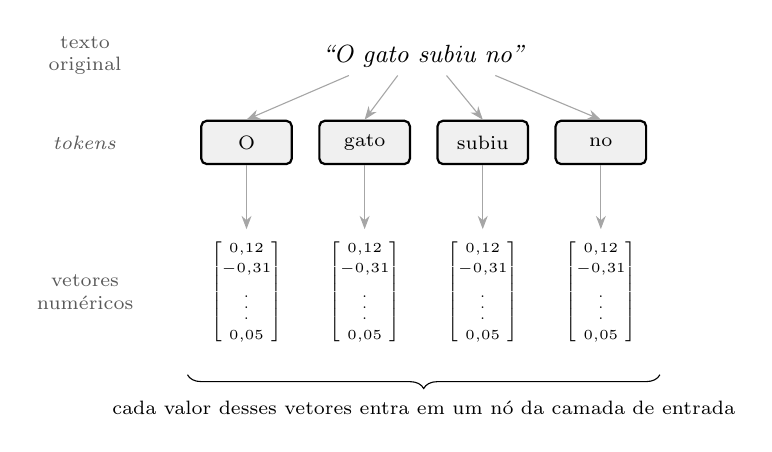
\begin{tikzpicture}[font=\scriptsize]
  % ---- a frase ----
  \node[font=\small] at (0,1.5) {\textit{``O gato subiu no''}};
  \node[font=\scriptsize,gray!70!black,align=center] at (-4.3,1.5) {texto\\ original};

  % ---- os tokens ----
  \foreach \i/\t in {0/O, 1/gato, 2/subiu, 3/no} {
    \node[draw,thick,rounded corners=2pt,fill=gray!12,
          minimum width=1.15cm,minimum height=0.55cm] (tk\i) at ({\i*1.5-2.25},0.4) {\t};
    \draw[-{Stealth},gray!70] ({\i*0.62-0.95},1.25) -- (tk\i.north);
  }
  \node[font=\scriptsize,gray!70!black,align=center] at (-4.3,0.4) {\textit{tokens}};

  % ---- os vetores ----
  \foreach \i in {0,...,3} {
    \node[font=\tiny] (em\i) at ({\i*1.5-2.25},-1.5)
      {$\begin{bmatrix} 0{,}12 \\ -0{,}31 \\ \vdots \\ 0{,}05 \end{bmatrix}$};
    \draw[-{Stealth},gray!70] (tk\i.south) -- (em\i.north);
  }
  \node[font=\scriptsize,gray!70!black,align=center] at (-4.3,-1.5) {vetores\\ numéricos};

  % ---- a camada de entrada ----
  \draw[decorate,decoration={brace,mirror,amplitude=5pt}] (-3.0,-2.55) -- (3.0,-2.55)
    node[midway,below=6pt,font=\scriptsize,align=center]
    {cada valor desses vetores entra em um nó da camada de entrada};
\end{tikzpicture}
\fonte{.}
\end{figure}

\modificado{O ciclo de treinamento pode ser resumido nos seguintes passos \cite{Goodfellow2016}:}
\begin{itemize}
    \item \textbf{Passo 1 -- Inicialização dos parâmetros:} pesos são inicializados com valores aleatórios baixos e \textit{biases} com zero. Essa quebra de simetria permite que diferentes neurônios aprendam características distintas.
    \item \textbf{Passo 2 -- \textit{Forward pass}:} um lote de dados é inserido na camada de entrada e propagado através das camadas ocultas até a camada de saída, produzindo uma predição.
    \item \textbf{Passo 3 -- Cálculo da perda:} a predição é comparada com o rótulo verdadeiro por meio de uma função de perda, que quantifica numericamente o quão distante a predição está do valor correto.
    \item \textbf{Passo 4 -- \textit{Backpropagation}:} o erro é propagado de volta pela rede, calculando-se o gradiente da função de perda em relação a cada peso e \textit{bias}.
    \item \textbf{Passo 5 -- Atualização dos parâmetros:} um otimizador atualiza pesos e \textit{biases} na direção oposta ao gradiente, reduzindo a função de perda.
    \item \textbf{Passo 6 -- Repetição:} os passos 2 a 5 são repetidos para cada lote e ao longo de um número definido de épocas.
\end{itemize}
\modificado{O treinamento é interrompido quando o modelo atinge uma precisão satisfatória ou quando a função de perda deixa de diminuir significativamente.}

% Seção "Arquitetura Transformer" mantida em arquivo próprio para revisão isolada.
% Integrada aqui, antes de "Consumo Energético", conforme planejado.
% =====================================================================
% SEÇÃO: Arquitetura Transformer (para integrar ao Capítulo 2)
% Criada em rodada separada para revisão isolada.
% Integrar posteriormente em 02_capitulo/fundamentacao_teorica.tex,
% idealmente ANTES da seção "Consumo Energético em Redes Neurais".
% =====================================================================

\section{Arquitetura Transformer}\label{sec:transformer}

A arquitetura \textit{Transformer}, proposta por \citeonline{Vaswani2017} no trabalho
\textit{Attention is All You Need}, marcou uma mudança profunda na forma como modelos
de aprendizado profundo processam sequências de texto. Antes dessa proposta, o campo
era dominado por arquiteturas que processavam a sequência elemento por elemento, palavra
por palavra. O \textit{Transformer} rompeu com essa abordagem ao introduzir um mecanismo
capaz de considerar toda a sequência de uma só vez. Esta seção apresenta, de forma
progressiva, os conceitos necessários para compreender a arquitetura utilizada neste
trabalho: as limitações das abordagens anteriores, o mecanismo de atenção, a operação
de autoatenção e sua versão multi-cabeça, a estrutura de cada bloco da rede e,
finalmente, o modelo GPT-2, que é o objeto central dos experimentos de poda.

% COLOCAR FIGURA: diagrama simplificado comparando o processamento sequencial de
% uma RNN (palavras processadas uma a uma, da esquerda para a direita) com o
% processamento paralelo do Transformer (todas as palavras conectadas entre si
% simultaneamente). Elaboração própria.

\subsection{Limitações das Arquiteturas Recorrentes}\label{subsec:limitacoes_rnn}

Até a chegada do \textit{Transformer}, o processamento de texto era dominado pelas redes
neurais recorrentes (\textit{Recurrent Neural Networks}, RNNs), popularizadas ao longo da
década de 1990. Diferentemente de arquiteturas puramente diretas, as RNNs processam a
sequência palavra por palavra e reaproveitam a saída de cada passo como entrada do passo
seguinte, criando uma forma de ``memória'': a cada nova palavra, um estado oculto
(\textit{hidden state}) é atualizado com base na palavra atual e no estado anterior, de
modo que, ao final, ele deve resumir as informações relevantes de todo o texto.

Essa memória, porém, falha em sequências longas. Considere o trecho ``A Inglaterra é minha
terra natal. Passei toda a minha vida lá. Mudei-me para a Espanha há dois dias. Eu falo
apenas uma língua, que é o \_\_\_''. Para completar a lacuna corretamente com ``inglês'', o
modelo precisa recuperar a palavra ``Inglaterra'', que aparece no início do trecho. O
obstáculo é o chamado gradiente desaparecente (\textit{vanishing gradient}): durante o
treinamento via \textit{backpropagation}, os gradientes são multiplicados repetidamente
pelas matrizes de peso da rede e, quando esses valores são pequenos, encolhem até se
aproximarem de zero \cite{Bengio1994}. Com isso, a influência de ``Inglaterra'' torna-se
insignificante ao chegar à lacuna, e o modelo perde o contexto necessário --- limitação
que se manifesta como incapacidade de lidar com \textbf{dependências de longo alcance}.

Há ainda uma segunda limitação, de ordem computacional: como o estado oculto no instante
$t$ só pode ser calculado após o do instante $t-1$, o processamento é estritamente
sequencial e mal aproveita o paralelismo das unidades de processamento gráfico (GPUs)
modernas. Essas duas dificuldades impulsionaram uma evolução cronológica de arquiteturas.
As redes LSTM (\textit{Long Short-Term Memory}), propostas em 1997, atacaram o gradiente
desaparecente por meio de portas (\textit{gates}) que regulam o que deve ser mantido ou
esquecido, permitindo reter por mais tempo informações como ``Inglaterra''
\cite{Hochreiter1997}. Ainda assim, as LSTMs continuam processando a frase de forma
sequencial, o que as mantém lentas e difíceis de paralelizar em grandes volumes de dados
--- gargalo que só seria superado pelo mecanismo de atenção.

% SUGESTÃO DE FIGURA: diagrama mostrando uma RNN processando a frase de exemplo,
% com setas indicando o fluxo do estado oculto e destacando a "distância" entre
% "Inglaterra" e a lacuna final. Elaboração própria.

\subsection{Mecanismo de Atenção}\label{subsec:atencao}

O passo seguinte dessa evolução foi o mecanismo de atenção (\textit{attention
mechanism}), introduzido por \citeonline{Bahdanau2015} no contexto da tradução automática.
Em vez de comprimir toda a frase em um único estado oculto, a atenção permite que o modelo
``olhe'' de volta e foque seletivamente em partes específicas da entrada. No exemplo
anterior, ela pode consultar diretamente o termo ``Inglaterra'', independentemente de quão
distante ele esteja da lacuna, eliminando o risco de o gradiente desaparecer pelo caminho.

Para operacionalizar essa ideia, o mecanismo utiliza três conceitos: a consulta
(\textit{query}), a chave (\textit{key}) e o valor (\textit{value}). Uma analogia útil é a
de uma biblioteca: cada livro tem uma etiqueta na lombada (a \textit{chave}) que descreve
seu conteúdo; quando um leitor chega com uma pergunta (a \textit{consulta}), ela é comparada
com cada etiqueta para decidir quais livros são mais relevantes; o conteúdo desses livros
(os \textit{valores}) é então combinado, com os mais relevantes contribuindo mais para a
resposta. No \textit{Transformer}, esse processo ocorre com números: a relevância entre uma
consulta e cada chave é calculada matematicamente, e os valores são somados com pesos
proporcionais a essa relevância.

A inovação central de \citeonline{Vaswani2017}, em 2017, foi construir uma arquitetura
inteira baseada exclusivamente nesse mecanismo, dispensando por completo a recorrência.
Com isso, todas as posições de uma sequência se comunicam diretamente em uma única
operação, sem precisar ``passar'' por palavras intermediárias. Isso resolve as duas
limitações das RNNs de uma só vez: as dependências de longo alcance tornam-se tão fáceis
de capturar quanto as de curto alcance, e o cálculo passa a ser paralelizável, tornando
as arquiteturas baseadas em RNN e LSTM obsoletas para muitas tarefas modernas.

\subsection{Autoatenção e Atenção Multi-Cabeça}\label{subsec:autoatencao}

A variante do mecanismo de atenção utilizada no \textit{Transformer} é chamada de
autoatenção (\textit{self-attention}). O prefixo ``auto'' indica que a consulta, a chave
e o valor são todos derivados da mesma sequência de entrada. Ou seja,
ao processar uma frase, cada palavra pergunta a si mesma: ``quais outras palavras desta
frase são relevantes para minha interpretação?''. Exemplo: ``O gato que estava
no telhado dormiu''. Ao processar a palavra ``dormiu'', o mecanismo de autoatenção
calcula um peso para cada palavra da frase. A palavra ``gato'' recebe peso alto, pois é
o sujeito do verbo; palavras como ``telhado'' ou ``no'' recebem pesos baixos, pois são
menos relevantes para determinar quem dormiu.

Na prática, esses pesos são calculados da seguinte forma, a partir de cada representação
de entrada, três matrizes de pesos aprendíveis durante o treinamento transformam cada
representação em três vetores: o vetor de consulta $Q$ (\textit{query}), o vetor de
chave $K$ (\textit{key}) e o vetor de valor $V$ (\textit{value}). O grau de compatibilidade
entre uma consulta e cada chave é calculado pelo produto escalar entre eles. Esses valores
brutos de compatibilidade passam pela função \textit{softmax}, que os converte em uma
distribuição de probabilidades, isto é, um conjunto de números entre 0 e 1 que somam
exatamente 1. Esses pesos normalizados determinam com que intensidade cada valor $V$
contribui para o resultado final, que é obtido pela soma ponderada dos valores.

Essa operação completa é denominada \textit{Scaled Dot-Product Attention} (atenção por
produto escalar escalado) e é definida formalmente por \cite{Vaswani2017}:

\[
    \text{Attention}(Q, K, V) = \text{softmax}\!\left(\frac{QK^\top}{\sqrt{d_k}}\right) V
\]

Em termos intuitivos, o produto $QK^\top$ mede a compatibilidade entre todas as consultas e
todas as chaves de uma só vez; a divisão por $\sqrt{d_k}$ (a dimensão das chaves) é um fator
de escala que estabiliza o treinamento; a \textit{softmax} converte essas pontuações em
pesos que somam 1; e a multiplicação por $V$ produz, para cada posição, uma média ponderada
dos valores, isto é, sua representação já contextualizada pelo restante da sequência.

Uma única operação de atenção, porém, captura apenas um tipo de relação entre as palavras
de cada vez. Para superar essa limitação, \citeonline{Vaswani2017} propõem a atenção
multi-cabeça (\textit{multi-head attention}). A analogia é a seguinte: se a atenção
simples é como um único leitor relendo a frase em busca de relações gramaticais, a atenção
multi-cabeça é como $h$ leitores independentes, cada um procurando um tipo diferente de
relação. Um leitor pode focar em concordância verbal (``gato''/``dormiu''), outro em
relações de posse (``telhado do vizinho''), outro em referências pronominais, e assim por
diante. O GPT-2 \textit{small}, por exemplo, utiliza 12 cabeças de atenção por bloco.

Na prática, cada uma das $h$ cabeças executa a operação \textit{Scaled Dot-Product
Attention} de forma independente, com suas próprias matrizes de projeção aprendíveis para
$Q$, $K$ e $V$. As saídas das $h$ cabeças são depois concatenadas e projetadas por uma
matriz linear aprendível, produzindo a representação final de cada posição. Desse modo,
o modelo pode simultaneamente capturar relações em diferentes subespaços semânticos e
sintáticos, sem custo adicional expressivo em relação à atenção simples.

Sob a perspectiva da compressão de modelos, as cabeças de atenção constituem unidades
podáveis naturais para a poda estruturada: estudos da literatura demonstram que nem todas
as cabeças são igualmente úteis, e que algumas podem ser removidas inteiramente sem
degradação significativa da qualidade das predições \cite{Michel2019}. 
% Essa propriedade
% é explorada diretamente nos experimentos deste trabalho.

% SUGESTÃO DE FIGURA: diagrama comparativo entre Scaled Dot-Product Attention (esquerda,
% mostrando Q, K, V, o produto escalar, a softmax e a ponderação de V) e Multi-Head
% Attention (direita, mostrando h cabeças paralelas com concatenação e projeção final),
% adaptado de Vaswani et al. (2017), Fig. 2.

\subsection{Estrutura do Bloco Transformer}\label{subsec:bloco_transformer}

Para entender como o \textit{Transformer} processa informação em profundidade, é útil
pensar em cada bloco como uma ``estação de trabalho'' em uma linha de montagem. Na
primeira bancada, as palavras trocam informações entre si por meio da atenção
multi-cabeça: cada palavra atualiza sua representação consultando todas as demais. Na
segunda bancada, cada palavra refina individualmente sua própria representação, de forma
independente das outras, por meio de uma pequena rede totalmente conectada.
Esse par de operações se repete em cada bloco, e os blocos são empilhados, fazendo com
que as representações das palavras se tornem progressivamente mais ricas e abstratas a
cada andar.

O primeiro bloco é a
camada de atenção multi-cabeça, já apresentada na seção anterior, responsável por
integrar informação contextual de toda a sequência. O segundo é uma rede
\textit{feedforward} totalmente conectada --- um MLP (\textit{multilayer perceptron})
aplicado de forma idêntica e independente a cada posição. Esse MLP é composto por duas
transformações lineares com uma função de ativação não linear entre elas: \modificado{a função GELU
(\textit{Gaussian Error Linear Unit}) \cite{Hendrycks2016} nos modelos GPT, ou ReLU em outras variantes.
\adicionadomarcelo{Diferentemente da ReLU \cite{Nair2010}, que simplesmente zera valores negativos, a
GELU faz uma transição suave em torno da origem. Na prática, essa suavidade evita o problema dos
``neurônios mortos'' (\textit{dying ReLU}), em que unidades deixam de aprender por receberem gradiente
nulo, e por isso \citeonline{Radford2019} a adotaram como ativação padrão na família GPT.}} A
dimensão intermediária desse MLP é tipicamente quatro vezes maior do que a dimensão
do modelo --- no GPT-2 \textit{small}, a dimensão do modelo é 768 e a dimensão
intermediária é 3.072 --- o que confere ao bloco grande capacidade de representação antes
de comprimir novamente a informação.

% Cada um dos dois sub-módulos é envolvido por dois mecanismos que facilitam o treinamento
% de modelos profundos. O primeiro é a conexão residual (\textit{residual connection}),
% idêntica em conceito à utilizada nas redes ResNet \cite{He2016}: a entrada do
% sub-módulo é somada diretamente à sua saída, criando um ``atalho'' que permite ao gradiente
% fluir mais facilmente para camadas anteriores durante o \textit{backpropagation}. O leitor
% familiarizado com arquiteturas convolucionais reconhecerá esse mecanismo. O segundo é a
% normalização de camada (\textit{layer normalization}), que estabiliza as ativações ao
% longo do treinamento, normalizando-as ao longo da dimensão das representações em vez da
% dimensão do lote, tornando o treinamento mais estável e menos sensível à taxa de
% aprendizado.

% A arquitetura completa de um modelo baseado em \textit{Transformer} consiste em um número
% $L$ de blocos empilhados. O GPT-2 \textit{small} possui $L = 12$ blocos. Cada bloco
% adicional aumenta a capacidade do modelo de aprender representações mais abstratas, da
% mesma forma que camadas mais profundas em uma rede convolucional capturam características
% visuais progressivamente mais complexas. Essa profundidade, porém, vem com custo
% computacional e energético proporcional: cada bloco extra adiciona parâmetros e operações
% ao caminho de cada inferência.

% Do ponto de vista da compressão, essa organização modular expõe múltiplos alvos para a
% poda estruturada: os neurônios intermediários da camada MLP (que podem ser removidos
% reduzindo a dimensão intermediária), as cabeças de atenção (que podem ser eliminadas
% inteiramente) e, em cenários de compressão mais agressiva, blocos \textit{Transformer}
% inteiros. Essa variedade de alvos torna a poda estruturada em modelos \textit{Transformer}
% mais rica em granularidade do que em redes convolucionais como a ResNet-50, onde os
% alvos típicos são filtros e canais de convolução \cite{Li2017}.

% SUGESTÃO DE FIGURA: diagrama de um único bloco Transformer (decoder-only), mostrando
% a camada de atenção multi-cabeça, a camada MLP feedforward, as conexões residuais e
% a normalização de camada, com as dimensões do GPT-2 small anotadas (768, 3072, 12 cabeças).
% Elaboração própria.

\subsection{Modelos de Linguagem de Grande Escala e o GPT-2}\label{subsec:llm_gpt2}

Modelos de linguagem de grande escala (\textit{Large Language Models}, LLMs) são redes
neurais profundas, tipicamente baseadas na arquitetura \textit{Transformer}, treinadas em
grandes volumes de texto com o objetivo de aprender a prever palavras. A tarefa de
pré-treinamento é simples de enunciar: dado um trecho de texto, o modelo deve prever
qual token vem a seguir. Um \textit{token} é a unidade mínima de texto que o modelo
processa --- pode ser uma palavra, parte de uma palavra, um sinal de pontuação ou um
espaço. Dada a sequência ``O aluno abriu o'', um LLM bem treinado atribuiria alta
probabilidade a tokens como ``livro'', ``caderno'' ou ``computador'', e baixa probabilidade
a tokens como ``foguete'' ou ``plutônio''. Repetida bilhões de vezes sobre textos variados,
essa tarefa aparentemente simples força o modelo a aprender gramática, fatos sobre o mundo,
raciocínio básico e muito mais \cite{Radford2019}.

Para que o texto possa ser processado numericamente, ele precisa primeiro ser convertido
em tokens e depois em vetores numéricos. Essa conversão ocorre em duas etapas. A primeira
é a tokenização, realizada por algoritmos como o BPE (\textit{Byte Pair Encoding}), que
divide o texto em unidades de comprimento variável de forma a equilibrar cobertura e
eficiência. Por exemplo, a palavra ``inconstitucional'' pode ser dividida em tokens como
``in'', ``constitu'' e ``cional''. O GPT-2 possui um vocabulário de aproximadamente
50.257 tokens. A segunda etapa converte cada token em um vetor numérico denso por meio
de uma camada de \textit{embedding}: o modelo aprende, durante o treinamento, uma
representação vetorial para cada token do vocabulário, de modo que tokens semanticamente
próximos tendam a ter representações próximas no espaço vetorial.

O GPT-2 (\textit{Generative Pre-trained Transformer 2}), proposto por
\citeonline{Radford2019} pela OpenAI em 2019, é um modelo autorregressivo baseado
exclusivamente no componente decodificador do \textit{Transformer} original. Ele foi
pré-treinado em um corpus de aproximadamente 40 GB de texto coletado da internet,
abrangendo uma grande diversidade de domínios e estilos. A variante GPT-2 \textit{small},
utilizada neste trabalho, possui 12 blocos \textit{Transformer} empilhados, 12 cabeças de
atenção por bloco, dimensão de modelo igual a 768 e aproximadamente 124 milhões de
parâmetros treináveis. Apesar de ser a menor variante da família GPT-2, esse número de
parâmetros é cerca de 70 vezes maior do que o de uma ResNet-50 (25 milhões de
parâmetros), o que ilustra a escala característica dos modelos baseados em \textit{Transformer}.

O crescimento em escala dos LLMs ao longo dos anos seguintes foi vertiginoso: o GPT-3,
publicado em 2020, possui 175 bilhões de parâmetros; o PaLM, do Google, chega a 540
bilhões. Mesmo modelos de médio porte como o GPT-2 impõem custos energéticos e
computacionais consideráveis em ambientes de produção, onde a inferência é executada
milhares ou milhões de vezes por dia. A poda estruturada surge, nesse contexto, como uma
estratégia concreta para reduzir esses custos: a remoção de cabeças de atenção
redundantes e de neurônios MLP de baixa importância pode diminuir substancialmente a
contagem de operações por inferência, com impacto controlado sobre a qualidade das
predições \cite{Patterson2021}. 
% Esse potencial de redução do consumo energético via poda
% estruturada em modelos \textit{Transformer} é o foco central dos experimentos conduzidos
% neste trabalho.


\section{Consumo Energético em Redes Neurais}\label{sec:consumo_energetico}
\modificado{O avanço de técnicas e \textit{hardware} voltados ao treinamento de redes neurais, motivado pela busca por maior precisão, trouxe consigo um consumo de energia considerável e, consequentemente, uma significativa emissão de dióxido de carbono. \adicionadomarcelo{\citeonline{Strubell2019}} relatam, por exemplo, que o treinamento de um modelo \textit{transformer} com busca de arquitetura neural pode emitir cerca de 626.155 libras de $CO_2$, enquanto a emissão média de um automóvel ao longo de toda a sua vida útil é de aproximadamente 126.000 libras --- cerca de cinco vezes menos.}

\modificado{Esse custo energético concentra-se em duas etapas do ciclo de vida de um modelo: o treinamento e a inferência.}

\modificado{No treinamento, o modelo é alimentado com grandes volumes de dados e ajustado iterativamente pelo \textit{backpropagation}. Esse processo é computacionalmente intenso e geralmente requer \textit{hardware} especializado (GPUs ou TPUs), muitas vezes organizado em \textit{clusters} com centenas ou milhares de aceleradores \cite{Patterson2021,Schwartz2020}.}

\modificado{Na inferência, o modelo já treinado é utilizado para gerar predições. O custo de uma única predição é relativamente baixo; contudo, em contextos de larga escala --- como os modelos de IA generativa servindo milhões de requisições diárias --- o custo energético agregado é expressivo \cite{Luccioni2022}.}

A diferença entre as duas etapas é de natureza, não apenas de grandeza. O treinamento é um
gasto concentrado e único, comparável ao custo de construir uma ponte; a inferência é um
gasto pequeno, porém perpétuo, comparável ao custo de mantê-la aberta ao tráfego. Uma ponte
muito usada acaba custando, ao longo de décadas, mais em manutenção do que custou para ser
erguida --- e o mesmo ocorre com um modelo consultado milhões de vezes por dia. É por essa
razão que este trabalho concentra-se na eficiência da inferência.

\section{Compressão de Modelos}
\modificado{Com o crescimento do \textit{Deep Learning}, os modelos de IA vêm dobrando em tamanho a cada poucos anos \cite{Sevilla2022}. Modelos de alta performance costumam ser otimizados exclusivamente para acurácia, resultando em redes com grande quantidade de parâmetros, que ocupam muito espaço de armazenamento e demandam um elevado número de operações em ponto flutuante (FLOPs) para serem executadas. Isso é particularmente problemático em dispositivos com capacidade limitada, como \textit{smartphones} e sistemas embarcados, e também em contextos de uso em larga escala, nos quais o custo energético se torna significativo.}

\modificado{A compressão de modelos é um campo que reúne técnicas voltadas a atenuar esses problemas, reduzindo o tamanho dos modelos e/ou a quantidade de operações necessárias para sua execução, preservando, tanto quanto possível, a acurácia. As redes neurais modernas possuem alta redundância de parâmetros \cite{Denil2013}, o que torna viável remover ou simplificar aqueles com baixa contribuição ao resultado final.}

Essa redundância não é um defeito, mas uma consequência do modo como esses modelos são
construídos. Como não se sabe de antemão quantos parâmetros a tarefa exige, projeta-se a
rede com folga generosa, do mesmo modo que se dimensiona uma instalação elétrica para uma
carga muito acima da que será efetivamente usada. A folga facilita o treinamento, mas
permanece no modelo depois que ele já aprendeu --- e é justamente essa sobra que as
técnicas de compressão procuram eliminar.

\modificado{As quatro principais famílias de técnicas de compressão são:}
\begin{itemize}
    \item \textbf{Quantização (Quantization):} \modificado{reduz o número de \textit{bits} utilizados para representar cada peso do modelo. Em vez de pontos flutuantes de 32 bits, os parâmetros passam a ser representados com precisão reduzida (16 ou 8 bits, por exemplo), o que diminui o tamanho do modelo e pode acelerar operações em \textit{hardware} que suporta aritmética de menor precisão \cite{Jacob2018}. O equivalente cotidiano é anotar preços arredondados: registrar R\$ 20 em vez de R\$ 19,99 ocupa menos espaço e agiliza as contas, e na maioria das situações a diferença é irrelevante.}
    \item \textbf{Destilação de Conhecimento (Knowledge Distillation):} \modificado{proposta por \citeonline{Hinton2015}, é uma metodologia de treinamento em que um modelo menor (\textit{aluno}) aprende a partir de um modelo maior e mais preciso (\textit{professor}). O aluno é treinado não apenas para acertar os rótulos verdadeiros, mas também para imitar a distribuição de saída do professor, resultando em um modelo compacto que, frequentemente, alcança acurácia superior à que teria se fosse treinado do zero.}
    \item \textbf{Fatoração de Matrizes (Matrix Factorization):} \modificado{matrizes de pesos de grandes dimensões são decompostas em produto de matrizes menores cuja multiplicação aproxima a matriz original, reduzindo o custo computacional \cite{Denton2014}.}
    \item \textbf{Poda Neural (Neural Pruning):} \modificado{processo de remoção de pesos --- ou de estruturas maiores, como filtros --- que contribuem pouco para a saída do modelo. É a técnica central deste trabalho e será detalhada na Seção a seguir.}
\end{itemize}

\begin{figure}[htb]
\centering
\caption{\adicionadomarcelo{Ilustração do processo de poda: a rede original (densa) tem conexões e/ou neurônios removidos, tornando-se esparsa.}}
\label{fig:poda_ilustracao}
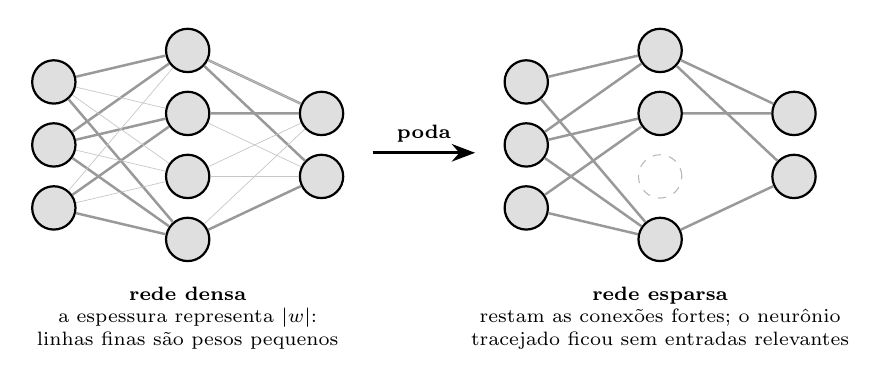
\begin{tikzpicture}[font=\scriptsize,
    neuronio/.style={circle,draw,thick,minimum size=5.5mm,inner sep=0,fill=gray!25},
    removido/.style={circle,draw,dashed,gray!55,minimum size=5.5mm,inner sep=0,fill=white}]

  % A espessura de cada conexão representa a magnitude do peso |w|: linhas
  % finas são pesos pequenos, os primeiros candidatos à remoção.
  \begin{scope}
    \foreach \i in {1,2,3} \node[neuronio] (a\i) at (0,{-\i*0.8}) {};
    \foreach \j in {1,2,3,4} \node[neuronio] (b\j) at (1.7,{-\j*0.8+0.4}) {};
    \foreach \k in {1,2} \node[neuronio] (c\k) at (3.4,{-\k*0.8-0.4}) {};
    % conexões fortes (peso alto)
    \foreach \i/\j in {1/1,1/4,2/1,2/2,2/4,3/2,3/4}
      \draw[gray!80,line width=0.9pt] (a\i) -- (b\j);
    \foreach \j/\k in {1/1,1/2,2/1,4/2}
      \draw[gray!80,line width=0.9pt] (b\j) -- (c\k);
    % conexões fracas (peso próximo de zero)
    \foreach \i/\j in {1/2,1/3,2/3,3/1,3/3}
      \draw[gray!45,line width=0.25pt] (a\i) -- (b\j);
    \foreach \j/\k in {1/1,2/2,3/1,3/2,4/1}
      \draw[gray!45,line width=0.25pt] (b\j) -- (c\k);
    \node[align=center] at (1.7,-3.8)
      {\textbf{rede densa}\\ a espessura representa $|w|$:\\ linhas finas são pesos pequenos};
  \end{scope}

  \draw[-{Stealth},very thick] (4.05,-1.7) -- (5.35,-1.7)
    node[midway,above,align=center] {\textbf{poda}};

  \begin{scope}[shift={(6.0,0)}]
    \foreach \i in {1,2,3} \node[neuronio] (d\i) at (0,{-\i*0.8}) {};
    \foreach \j in {1,2,4} \node[neuronio] (e\j) at (1.7,{-\j*0.8+0.4}) {};
    \node[removido] (e3) at (1.7,{-3*0.8+0.4}) {};
    \foreach \k in {1,2} \node[neuronio] (f\k) at (3.4,{-\k*0.8-0.4}) {};
    \foreach \i/\j in {1/1,1/4,2/1,2/2,2/4,3/2,3/4}
      \draw[gray!80,line width=0.9pt] (d\i) -- (e\j);
    \foreach \j/\k in {1/1,1/2,2/1,4/2}
      \draw[gray!80,line width=0.9pt] (e\j) -- (f\k);
    \node[align=center] at (1.7,-3.8)
      {\textbf{rede esparsa}\\ restam as conexões fortes; o neurônio\\ tracejado ficou sem entradas relevantes};
  \end{scope}
\end{tikzpicture}
\fonte{Adaptado de \citeonline{Han2015}.}
\end{figure}

\section{Poda Neural (Pruning)}\label{sec:pruning}
\modificado{A poda neural é uma técnica de compressão que visa reduzir o tamanho do modelo e o custo computacional da inferência por meio da remoção de parâmetros que pouco contribuem para o resultado final. O processo mais comum parte de um modelo previamente treinado, cujo foco inicial foi exclusivamente a acurácia, e aplica a poda como uma etapa posterior \cite{Han2015,Blalock2020}.}

% O termo é emprestado da jardinagem, e a metáfora é precisa: podar uma árvore consiste em
% cortar os galhos que consomem seiva sem produzir frutos, de modo que a planta fique mais
% leve e continue rendendo o mesmo. A dificuldade, tanto no jardim quanto na rede neural,
% está em identificar com segurança quais galhos são realmente dispensáveis --- e é essa
% pergunta que separa as diferentes estratégias de poda apresentadas a seguir.

\subsection{Tipos de Poda}
\modificado{Na literatura, duas categorias principais de poda são consideradas \cite{Blalock2020}:}
\begin{itemize}
    \item \textbf{Poda não estruturada:} remoção de pesos individuais, independentemente da sua posição na matriz de pesos. Esta abordagem oferece maior flexibilidade e, geralmente, taxas de compressão elevadas com perda reduzida de acurácia. Entretanto, \adicionadomarcelo{do ponto de vista do custo de inferência, a poda não estruturada apresenta uma limitação importante: processadores e GPUs convencionais não são eficientes em pular multiplicações por zero espalhadas de forma aleatória na matriz de pesos. Assim, embora o modelo tenha muitos zeros, as operações ainda são executadas, e o ganho prático de velocidade e energia tende a ser marginal, a menos que se utilize \textit{hardware} especializado ou formatos de armazenamento esparso.}
    \item \textbf{Poda estruturada:} remoção de estruturas inteiras, como neurônios, filtros ou canais convolucionais, o que implica a remoção completa de detectores de características. Como o resultado é uma matriz menor e ainda densa, há um ganho direto de velocidade e eficiência em \textit{hardware} convencional. O custo dessa abordagem é uma potencial perda maior de acurácia para uma mesma taxa de compressão.
\end{itemize}

\begin{figure}[htb]
\centering
\caption{\adicionadomarcelo{As duas categorias de poda aplicadas à mesma matriz de pesos. Na poda não estruturada os pesos removidos são apenas zerados e a matriz conserva suas dimensões; na poda estruturada, colunas inteiras são eliminadas e a matriz encolhe de fato.}}
\label{fig:nao_estruturada_vs_estruturada}
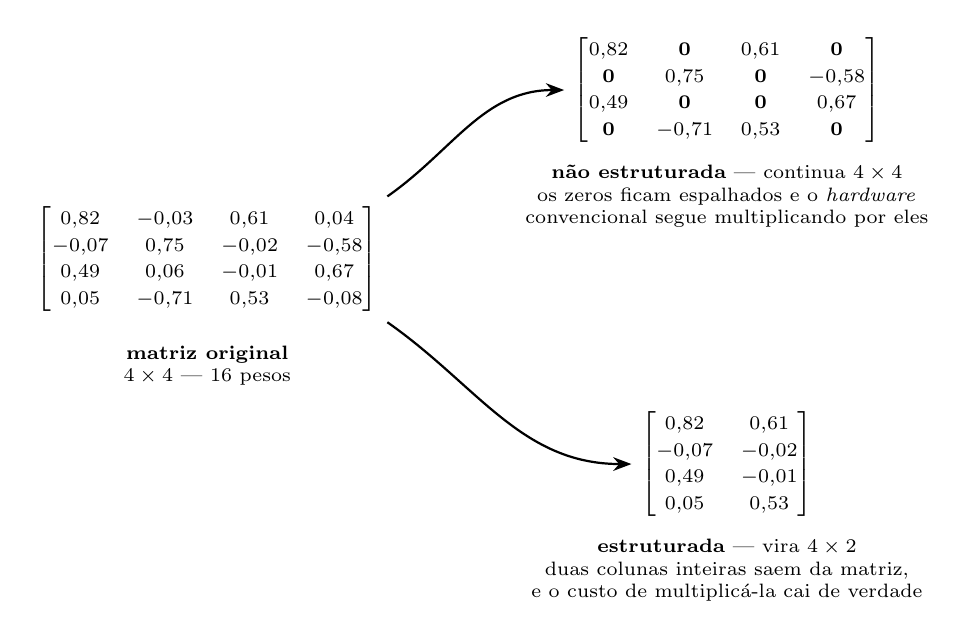
\begin{tikzpicture}[font=\scriptsize]
  % ---------- matriz original ----------
  \node (orig) at (0,0) {$\begin{bmatrix}
     0{,}82 & -0{,}03 &  0{,}61 &  0{,}04 \\
    -0{,}07 &  0{,}75 & -0{,}02 & -0{,}58 \\
     0{,}49 &  0{,}06 & -0{,}01 &  0{,}67 \\
     0{,}05 & -0{,}71 &  0{,}53 & -0{,}08
  \end{bmatrix}$};
  \node[below=5pt of orig,align=center] {\textbf{matriz original}\\ $4\times4$ --- 16 pesos};

  % ---------- poda não estruturada ----------
  \node (ne) at (6.6,2.15) {$\begin{bmatrix}
     0{,}82 & \mathbf{0} &  0{,}61 & \mathbf{0} \\
    \mathbf{0} &  0{,}75 & \mathbf{0} & -0{,}58 \\
     0{,}49 & \mathbf{0} & \mathbf{0} &  0{,}67 \\
    \mathbf{0} & -0{,}71 &  0{,}53 & \mathbf{0}
  \end{bmatrix}$};
  \node[below=1pt of ne,align=center]
    {\textbf{não estruturada} --- continua $4\times4$\\
     os zeros ficam espalhados e o \textit{hardware}\\ convencional segue multiplicando por eles};

  % ---------- poda estruturada ----------
  \node (es) at (6.6,-2.6) {$\begin{bmatrix}
     0{,}82 &  0{,}61 \\
    -0{,}07 & -0{,}02 \\
     0{,}49 & -0{,}01 \\
     0{,}05 &  0{,}53
  \end{bmatrix}$};
  \node[below=1pt of es,align=center]
    {\textbf{estruturada} --- vira $4\times2$\\
     duas colunas inteiras saem da matriz,\\ e o custo de multiplicá-la cai de verdade};

  % saem dos cantos (e não do centro) para não cruzar o rótulo da matriz
  \draw[-{Stealth},thick] (orig.north east) to[out=35,in=180] (ne.west);
  \draw[-{Stealth},thick] (orig.south east) to[out=-35,in=180] (es.west);
\end{tikzpicture}
% \fonte{Elaborada pelo autor.}
\end{figure}

A distinção entre as duas categorias é o que separa um ganho real de um ganho apenas
contábil, e uma analogia com um livro a torna evidente. A poda não estruturada equivale a
apagar palavras espalhadas por todas as páginas: o texto fica mais enxuto, mas o livro
continua com o mesmo número de páginas, e quem for lê-lo ainda terá de folhear todas elas
--- inclusive as partes apagadas. A poda estruturada equivale a arrancar capítulos
inteiros: o livro encolhe de fato, pesa menos e é percorrido em menos tempo. Como o
\textit{hardware} convencional não sabe pular um espaço em branco no meio de uma
multiplicação, apenas a segunda forma se converte em redução efetiva de tempo e de energia.
Essa diferença é retomada no Capítulo~\ref{chap:resultados}, onde é verificada
experimentalmente.

\adicionadomarcelo{Cabe mencionar também a chamada esparsidade estruturada (por exemplo, padrões 2:4), em que o algoritmo é forçado a zerar, a cada bloco de quatro pesos, exatamente dois. Como o \textit{hardware} sabe previamente quantos e em que formato os zeros aparecem, a matriz pode ser comprimida de maneira determinística, permitindo acelerações reais em GPUs modernas que suportam esse padrão \cite{NVIDIA2020Ampere}.}

\modificado{Assim, a poda estruturada é a que apresenta benefícios mais imediatos em termos de FLOPs e consumo de energia em \textit{hardware} convencional \cite{Li2017}, razão pela qual ela recebe destaque neste trabalho.}

\subsection{Poda por Magnitude}
\modificado{A técnica mais simples e amplamente estudada é a poda por magnitude. Nela, considera-se que pesos cujos valores absolutos são próximos de zero contribuem pouco para a saída do modelo e, portanto, podem ser removidos. Define-se um limiar (ou uma taxa de esparsidade desejada) e todos os pesos abaixo desse limiar são zerados, criando redes esparsas \cite{Han2015}.}

\begin{figure}[htb]
\centering
\caption{\adicionadomarcelo{Pipeline clássico de poda por magnitude: treinamento do modelo denso, remoção dos pesos de menor magnitude e retreinamento (\textit{fine-tuning}) dos pesos remanescentes.}}
\label{fig:poda_magnitude}
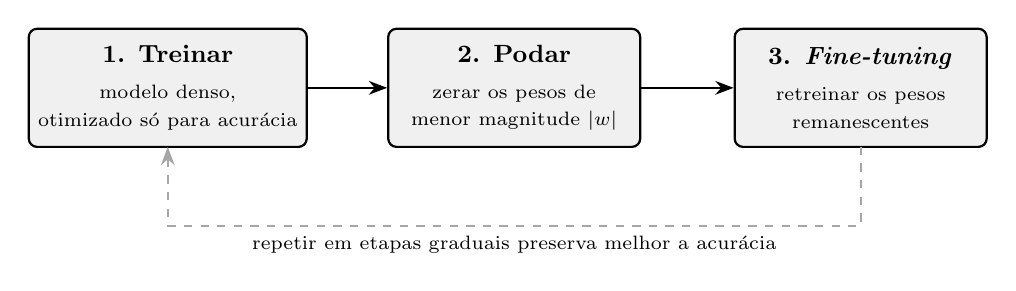
\begin{tikzpicture}[font=\small,
    etapa/.style={rectangle,rounded corners=3pt,draw,thick,fill=gray!12,
                  minimum width=3.2cm,minimum height=1.5cm,align=center}]
  \node[etapa] (t) at (0,0) {\textbf{1. Treinar}\\[2pt]
        \scriptsize modelo denso,\\[-1pt]\scriptsize otimizado só para acurácia};
  \node[etapa] (p) at (4.4,0) {\textbf{2. Podar}\\[2pt]
        \scriptsize zerar os pesos de\\[-1pt]\scriptsize menor magnitude $|w|$};
  \node[etapa] (f) at (8.8,0) {\textbf{3. \textit{Fine-tuning}}\\[2pt]
        \scriptsize retreinar os pesos\\[-1pt]\scriptsize remanescentes};

  \draw[-{Stealth},thick] (t) -- (p);
  \draw[-{Stealth},thick] (p) -- (f);

  % laço de iteração: desce do bloco 3, atravessa por baixo e sobe no bloco 1
  \draw[-{Stealth},thick,dashed,gray!70]
       (8.8,-0.75) -- (8.8,-1.75)
       -- node[below,font=\scriptsize,black]
          {repetir em etapas graduais preserva melhor a acurácia} (0,-1.75)
       -- (0,-0.75);
\end{tikzpicture}
\fonte{Adaptado de \citeonline{Han2015}.}
\end{figure}


\subsection{Sensibilidade e a Alocação do Orçamento de Poda}\label{subsec:sensibilidade}

A poda por magnitude responde a uma pergunta: \textit{quais} pesos remover. Ela deixa
intocada uma segunda pergunta, logicamente anterior e menos discutida: \textit{quanto}
remover de cada parte da rede. Um modelo com doze camadas e um orçamento de poda de
30\,\% admite infinitas distribuições desse orçamento --- 30\,\% em cada camada, 60\,\% na
metade delas e nada na outra metade, ou qualquer combinação intermediária. Todas removem a
mesma quantidade de parâmetros e produzem modelos de custo praticamente idêntico, mas não
produzem modelos de qualidade idêntica.

A analogia é a de uma empresa que precisa cortar 30\,\% das despesas. O corte linear ---
30\,\% em todos os setores --- é o mais simples de justificar e o que exige menos
informação, mas trata a contabilidade e a produção como igualmente dispensáveis. Um corte
melhor exige saber de antemão qual setor a empresa suporta perder e qual a paralisa. Essa
informação não está no orçamento de cada setor: um setor caro pode ser supérfluo, e um
setor barato pode ser crítico. Ela só aparece quando se pergunta o que acontece com a
empresa na ausência de cada setor.

É exatamente essa a definição de \textbf{sensibilidade} adotada neste trabalho: a
sensibilidade de uma camada é o quanto o desempenho do modelo se degrada quando aquela
camada, e somente ela, é podada. Trata-se de uma medida empírica e direta de importância,
obtida por ablação, e não de um \textit{proxy}. A distinção em relação à magnitude é
central: a magnitude é uma propriedade dos pesos, disponível sem custo algum, mas apenas
correlacionada com a importância; a sensibilidade é uma propriedade medida do
comportamento do modelo, cara de obter, porém direta.

\begin{figure}[htb]
\centering
\caption{Duas distribuições do mesmo orçamento de poda entre as camadas de uma rede. À
esquerda, a alocação uniforme, que ignora qualquer medida de importância; à direita, a
alocação guiada por sensibilidade, que poupa as camadas mais sensíveis e compensa nas mais
robustas. Ambas removem a mesma fração total de parâmetros. Figura esquemática.}
\label{fig:alocacao_sensibilidade}
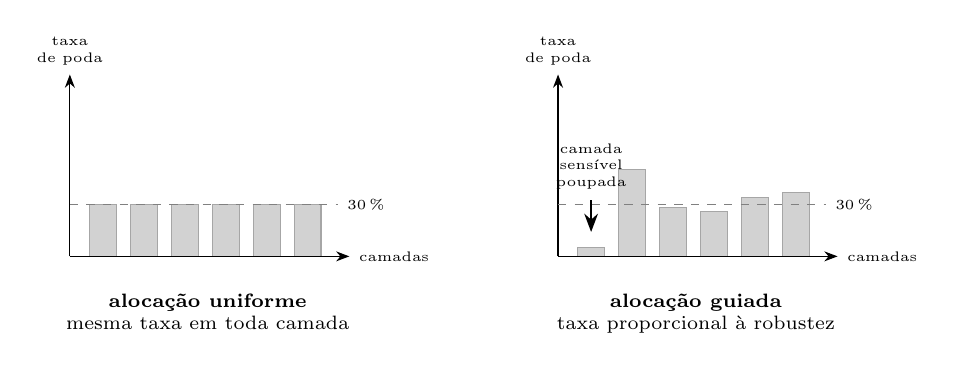
\begin{tikzpicture}[font=\scriptsize]
  \def\bw{0.34}   % largura da barra
  \def\sx{0.52}   % espaçamento horizontal
  \def\h{2.2}     % altura de referência (100%)

  % ---------- alocação uniforme ----------
  \begin{scope}
    \foreach \i in {0,...,5}{
      \draw[fill=gray!35,draw=gray!70] (\i*\sx,0) rectangle ++(\bw,{0.30*\h});
    }
    \draw[-{Stealth}] (-0.25,0) -- (3.3,0) node[right,font=\tiny] {camadas};
    \draw[-{Stealth}] (-0.25,0) -- (-0.25,{1.05*\h}) node[above,font=\tiny,align=center] {taxa\\de poda};
    \draw[dashed,gray] (-0.25,{0.30*\h}) -- (3.15,{0.30*\h})
         node[right,font=\tiny,black] {30\,\%};
    \node[below,align=center] at (1.5,-0.35) {\textbf{alocação uniforme}\\ mesma taxa em toda camada};
  \end{scope}

  % ---------- alocação guiada ----------
  \begin{scope}[xshift=6.2cm]
    % taxas ilustrativas com média 30%
    \foreach \i/\r in {0/0.05, 1/0.50, 2/0.28, 3/0.26, 4/0.34, 5/0.37}{
      \draw[fill=gray!35,draw=gray!70] (\i*\sx,0) rectangle ++(\bw,{\r*\h});
    }
    \draw[-{Stealth}] (-0.25,0) -- (3.3,0) node[right,font=\tiny] {camadas};
    \draw[-{Stealth}] (-0.25,0) -- (-0.25,{1.05*\h}) node[above,font=\tiny,align=center] {taxa\\de poda};
    \draw[dashed,gray] (-0.25,{0.30*\h}) -- (3.15,{0.30*\h})
         node[right,font=\tiny,black] {30\,\%};
    \draw[-{Stealth},thick] (0.17,{0.05*\h+0.15}) ++(0,0.45) -- ++(0,-0.4);
    \node[above,font=\tiny,align=center] at (0.17,{0.05*\h+0.62}) {camada\\sensível\\poupada};
    \node[below,align=center] at (1.5,-0.35) {\textbf{alocação guiada}\\ taxa proporcional à robustez};
  \end{scope}
\end{tikzpicture}
% \fonte{Elaborada pelo autor.}
\end{figure}

A ideia de medir importância por degradação não é nova. Ela remonta ao \textit{Optimal
Brain Damage} de \citeonline{LeCun1990}, que estima, por aproximação de segunda ordem, o
aumento de erro provocado pela remoção de cada peso, e ordena os parâmetros por essa
estimativa em vez de por magnitude. A limitação do método é o custo: a aproximação exige
informação de curvatura, cujo cálculo é proibitivo em redes com centenas de milhões de
parâmetros. A alternativa adotada aqui troca a estimativa analítica por medição direta e
reduz drasticamente a granularidade --- em vez de estimar a importância de cada peso
individualmente, mede-se a de cada camada. Com doze camadas, o perfil completo custa doze
avaliações do modelo, sem nenhum treinamento envolvido.

Há evidência consolidada de que essa desigualdade entre partes da rede existe e é
substancial. \citeonline{Denil2013} mostram que uma fração pequena dos parâmetros de uma
rede é suficiente para predizer todos os demais, o que indica redundância distribuída de
forma desigual. Em \textit{Transformers} especificamente, \citeonline{Michel2019}
verificam que a maioria das cabeças de atenção pode ser removida após o treinamento com
perda pequena de desempenho, enquanto algumas poucas são indispensáveis --- e que quais
delas são indispensáveis não é previsível a partir de propriedades dos pesos. Se a
importância fosse aproximadamente uniforme, a alocação do orçamento seria irrelevante e a
poda uniforme seria ótima por construção; é precisamente porque não é uniforme que existe
espaço para alocar melhor.

Duas ressalvas conceituais acompanham o método e delimitam o que ele pode oferecer.

A primeira é que a sensibilidade medida por ablação de uma camada por vez não captura
interações entre camadas. A degradação causada por podar duas camadas simultaneamente não
é, em geral, a soma das degradações individuais, de modo que o perfil deve ser tratado
como uma \textbf{ordenação relativa de robustez}, e não como um modelo capaz de prever a
qualidade de uma configuração completa. A segunda é que a sensibilidade não é uma
propriedade absoluta da camada: ela é medida em relação a uma estratégia de poda
específica, porque remover pesos de menor magnitude e remover cabeças de atenção inteiras
são operações diferentes, que danificam a camada de maneiras diferentes. O perfil precisa,
portanto, ser levantado uma vez para cada estratégia.

O procedimento que converte esse perfil em taxas de poda por camada é detalhado na
Seção~\ref{sec:estrategia_otimizada}, e ambas as ressalvas acima são verificadas
experimentalmente no Capítulo~\ref{chap:resultados}.

\subsection{Pipeline Geral da Poda}
\modificado{De forma geral, a poda pode ser dividida nos seguintes passos \cite{Blalock2020}:}
\begin{itemize}
    \item \textbf{Passo 1 -- Definição de critério e taxa de poda:} partindo de um modelo já treinado, define-se o critério de importância dos parâmetros (magnitude absoluta, norma $L_1$ de filtros, sensibilidade, entre outros) e a taxa de esparsidade desejada.
    \item \textbf{Passo 2 -- Identificação dos parâmetros a podar:} com base no critério escolhido, o algoritmo classifica os parâmetros por importância e seleciona os menos relevantes.
    \item \textbf{Passo 3 -- Execução da poda:} os parâmetros selecionados são zerados (no caso da poda não estruturada) ou fisicamente removidos (no caso da poda estruturada), gerando um modelo esparso ou uma nova arquitetura reduzida.
    \item \textbf{Passo 4 -- Ajuste fino (\textit{fine-tuning}):} como a remoção tende a deteriorar a acurácia, o modelo podado é retreinado com uma taxa de aprendizado reduzida, para que os parâmetros remanescentes compensem a ausência dos que foram removidos.
    \item \textbf{Passo 5 -- Iteração:} a poda pode ser aplicada de forma iterativa, em pequenas etapas intercaladas por \textit{fine-tuning}, o que costuma preservar melhor a acurácia do que uma poda agressiva em um único passo.
\end{itemize}

\subsection{Quando a Poda é Aplicada}
\modificado{Tradicionalmente, a poda é aplicada após o treinamento inicial do modelo, seguida de um ajuste fino. Métodos mais recentes aplicam a poda de forma gradual durante o próprio treinamento, intercalando passos de treino e poda, o que permite à rede adaptar-se progressivamente à nova estrutura \cite{Zhu2017}.}

\adicionadomarcelo{Uma linha de pesquisa mais recente investiga a possibilidade de podar a rede antes do treinamento, identificando sub-redes inerentemente promissoras dentro de uma rede densa inicializada aleatoriamente. Essa abordagem é impulsionada pela chamada \textit{Lottery Ticket Hypothesis} \cite{Frankle2019}, segundo a qual, dentro de uma rede grande inicializada aleatoriamente, existe uma sub-rede pequena (o ``bilhete premiado'') que, quando treinada isoladamente com a mesma inicialização, atinge acurácia comparável à da rede completa.}

% % =============================================================
% % Capítulo 3 — Trabalhos Relacionados
% % =============================================================

% \chapter{Trabalhos Relacionados}\label{chap:trabalhos_relacionados}

% \adicionadomarcelo{Este capítulo apresenta trabalhos da literatura diretamente relacionados ao tema desta pesquisa, com foco em estratégias de poda neural e, em especial, naquelas que visam a redução do consumo energético de modelos de \textit{Deep Learning}. Para cada trabalho, são descritos os objetivos principais, a metodologia adotada e os principais resultados obtidos.}

% \section{Designing Energy-Efficient Convolutional Neural Networks using Energy-Aware Pruning}\label{sec:yang2017}

% \modificado{\citeonline{Yang2017} propõem um algoritmo de poda para redes neurais convolucionais (CNNs) cujo foco é minimizar o consumo real de energia, e não apenas o número de parâmetros ou de operações, preservando a acurácia. Os autores consideram especialmente o custo computacional associado a operações de multiplicação e acumulação (MAC) e o custo de acesso à memória em dispositivos periféricos, como \textit{smartphones}.}

% \modificado{O método proposto aplica poda camada por camada, priorizando aquelas cujo consumo energético estimado é maior. Para isso, os autores desenvolvem um \textit{framework} de estimativa que ordena as camadas pela combinação de custo computacional (número de MACs) e custo de acesso à memória. Em cada camada podada, parte dos pesos é removida; em seguida, alguns pesos são restaurados para minimizar o erro no mapa de características de saída; por fim, os pesos remanescentes são ajustados localmente por meio de uma solução de mínimos quadrados. Após o processamento de todas as camadas, a rede passa por um \textit{fine-tuning} global utilizando \textit{backpropagation}.}

% \modificado{Os autores reportam redução de 3,7$\times$ no consumo de energia da AlexNet e 1,6$\times$ no da GoogLeNet, com perda de acurácia inferior a 1\%. O trabalho também demonstra empiricamente que as camadas convolucionais são as que mais consomem energia, principalmente devido ao volume de acessos à memória, e que a simples redução do número de classes tem impacto limitado na redução do consumo energético, uma vez que as camadas convolucionais não são significativamente afetadas.}

% \adicionadomarcelo{\todo[inline]{\textbf{A fazer:} adicionar resenhas de outros trabalhos fundamentais para esta pesquisa. Sugestões: \citeonline{Han2015} (poda por magnitude não estruturada -- seminal); \citeonline{Li2017} (poda estruturada L1 em filtros -- seminal); \citeonline{Frankle2019} (Lottery Ticket Hypothesis); \citeonline{Blalock2020} (revisão crítica de métodos de poda); \citeonline{Liu2019} (\textit{Rethinking the Value of Network Pruning}). Para cada um, seguir o mesmo padrão de resenha: objetivo, método, resultados principais.}}

% =============================================================
% Capítulo 4 — Metodologia
% =============================================================

\chapter{Metodologia}\label{chap:metodologia}

Este capítulo apresenta o percurso metodológico adotado no trabalho, organizado em cinco
etapas: a seleção do modelo de referência, a implementação das estratégias de poda sem
otimização, a implementação da estratégia de poda com otimização, o \textit{fine-tuning} de
recuperação e a definição das métricas de avaliação. Para cada etapa, estabelecem-se os
critérios que orientaram as decisões tomadas. As decisões concretas decorrentes desses
critérios --- incluindo o modelo selecionado, o \textit{dataset} empregado e as
configurações de poda --- são descritas no Capítulo~\ref{chap:desenvolvimento}.

% -------------------------------------------------------
\section{Seleção e Implementação do Modelo de Referência}\label{sec:metodologia_modelo}
% -------------------------------------------------------



O modelo de referência (\textit{baseline}) corresponde à versão original do modelo de linguagem
de grande escala (\textit{Large Language Model} --- LLM) antes de qualquer processo de poda.
Ele serve como padrão para mensurar a perda de desempenho introduzida pela compressão: todas as
métricas dos modelos podados são comparadas às métricas desse modelo original.

Para a seleção do modelo de referência, foram adotados os seguintes critérios:

\begin{itemize}
    \item ser um LLM representativo, amplamente utilizado na literatura de compressão de modelos;
    \item dispor de pesos pré-treinados publicamente disponíveis;
    \item apresentar tamanho compatível com as restrições de \textit{hardware} disponível;
    \item possuir ampla documentação em trabalhos de poda neural;
    \item \modificado{contar com implementação acessível em \textit{frameworks} consolidados,
          como PyTorch.}
\end{itemize}

% AJUSTE: reunião 13/05 — Hugging Face como plataforma, não biblioteca
\adicionadomarcelo{A implementação do modelo de referência utiliza a biblioteca PyTorch \cite{Paszke2019}.
Como repositório de modelos pré-treinados, é empregada a plataforma Hugging Face, um
ambiente colaborativo que disponibiliza ampla variedade de modelos de linguagem de grande
escala publicamente acessíveis --- como, por exemplo, variantes do GPT-2.
O modelo selecionado a partir dos critérios estabelecidos --- incluindo a versão específica
obtida via Hugging Face --- é apresentado e detalhado no
Capítulo~\ref{chap:desenvolvimento}.}

% -------------------------------------------------------
\section{Implementação das Estratégias de Poda sem Otimização}\label{sec:metodologia_poda_sem}
% -------------------------------------------------------


% AJUSTE: reunião 13/05 — duas estratégias (magnitude + estruturada), "avaliadas" em vez de "consideradas"
\adicionadomarcelo{As estratégias de poda sem otimização têm por objetivo reduzir o número de parâmetros de um
modelo pré-treinado, eliminando pesos ou estruturas avaliadas como menos relevantes para o
desempenho preditivo. Serão avaliadas duas estratégias de poda clássicas, escolhidas por
representarem os dois extremos do espectro de granularidade da poda neural:

\begin{itemize}
    \item poda baseada em magnitude dos pesos \cite{Han2015}, que remove parâmetros
          individuais cujos valores absolutos são inferiores a um limiar; representa a
          granularidade mais fina possível e gera modelos esparsos sem alteração da
          estrutura física do modelo;
    \item poda estruturada \cite{Li2017}, que elimina unidades arquiteturais inteiras
          --- filtros convolucionais, no trabalho original; em uma arquitetura
          \textit{Transformer}, cabeças de atenção ou neurônios da camada intermediária do
          MLP --- reduzindo fisicamente as dimensões dos tensores e gerando modelos
          computacionalmente mais enxutos.
\end{itemize}}

% AJUSTE: reunião 13/05 — reforçar que estratégias são consolidadas na literatura
\adicionadomarcelo{Ambas as estratégias são amplamente consolidadas na literatura de compressão de modelos
neurais, com mais de uma década de aplicação e extensa validação experimental. Sua inclusão
neste trabalho não constitui contribuição metodológica original; pelo contrário, sua
aplicação fornece uma base de comparação estabelecida, sobre a qual é avaliada a
estratégia otimizada proposta na
Seção~\ref{sec:metodologia_poda_com}.}

Os critérios que orientaram a escolha das estratégias a implementar foram:

\begin{itemize}
    \item representatividade na literatura de compressão de modelos;
    \item complementaridade entre granularidades distintas de remoção;
    \item viabilidade de implementação com as ferramentas disponíveis.
\end{itemize}


Em ambas as estratégias, são aplicadas funções de avaliação de importância de parâmetros,
que orientam o processo de remoção: a poda por magnitude utiliza como critério o valor
absoluto de cada peso individual, enquanto a poda estruturada utiliza a norma $L_1$ do
conjunto de pesos associado a cada unidade arquitetural removível.



As estratégias selecionadas com base nesses critérios, bem como os detalhes de sua
implementação, são apresentados no Capítulo~\ref{chap:desenvolvimento}.

% -------------------------------------------------------
% AJUSTE: reescrita da Seção 4.3 — a estratégia otimizada passa a ser declarada
% (sensibilidade por camada); taxas dinâmicas, momento de aplicação e Knowledge
% Distillation descem para alternativas descartadas, como no Cap. 5.
\section{Implementação da Estratégia de Poda com Otimização}\label{sec:metodologia_poda_com}
% -------------------------------------------------------

Esta é a etapa central do trabalho. O objetivo é investigar se a combinação de uma
estratégia clássica de poda com uma técnica de otimização resulta em modelos mais
eficientes do que a poda aplicada de forma direta, sem qualquer refinamento adicional.

A técnica de otimização adotada é a \textbf{análise de sensibilidade por camada}, que
orienta uma alocação não uniforme do orçamento de poda entre as camadas do modelo. A
hipótese que ela investiga é a de que as camadas não são igualmente importantes: se
algumas toleram a remoção de parâmetros muito mais do que outras, distribuir o orçamento
de poda em proporção a essa tolerância deve produzir, para um mesmo grau de compressão,
perda menor de desempenho preditivo do que as alocações ingênuas adotadas pelas
estratégias da Seção~\ref{sec:metodologia_poda_sem}.

O procedimento organiza-se em duas fases. Na primeira, levanta-se um perfil de
sensibilidade do modelo: poda-se uma camada de cada vez, a uma taxa fixa e mantendo todas
as demais intactas, e registra-se a degradação resultante na métrica de desempenho
preditivo. Na segunda, esse perfil é convertido em uma taxa de poda por camada, atribuída
em proporção à robustez medida e escalada de modo que o orçamento global pretendido seja
respeitado. Como cada estratégia de poda remove unidades de natureza distinta, o perfil é
levantado separadamente para cada uma delas. A formulação da regra de alocação, a
taxa-sonda empregada no perfilamento e os valores adotados para os demais parâmetros são
apresentados no Capítulo~\ref{chap:desenvolvimento}.

Os critérios que orientaram a escolha dessa técnica entre as alternativas cogitadas foram
sua aderência direta à hipótese do trabalho e o fato de não alterar a natureza da poda:
ela redistribui o orçamento entre as camadas sem modificar o critério de importância nem
introduzir um segundo modelo no experimento. Isso mantém a comparação com as estratégias
sem otimização restrita a uma única variável.

\subsection*{Alternativas consideradas e descartadas}

Outras técnicas de otimização foram cogitadas e não integram o escopo experimental, por
restrição de tempo. Registram-se a seguir, por delimitarem o alcance das conclusões e por
constituírem desdobramentos naturais para trabalhos futuros:

\begin{itemize}
    \item \textbf{comparação entre taxas de poda fixas e dinâmicas}, em que o orçamento de
          poda varia ao longo do processo em vez de ser fixado de antemão;
    \item \textbf{variação do momento de aplicação da poda} --- antes, durante ou após o
          treinamento. Este trabalho aplica a poda sempre sobre o modelo pré-treinado,
          reservando o retreinamento para a etapa de recuperação descrita na
          Seção~\ref{sec:metodologia_finetuning};
    \item \textbf{\textit{Knowledge Distillation}}, na qual um modelo menor
          (\textit{student}) é treinado para reproduzir o comportamento de um modelo maior
          (\textit{teacher}); trata-se de técnica de compressão de natureza distinta da
          poda, cuja avaliação exigiria protocolo experimental próprio;
    \item \textbf{quantização}, que reduz a precisão numérica da representação dos pesos
          em vez de eliminá-los.
\end{itemize}

A comparação entre os modelos obtidos com e sem otimização visa identificar em que medida
a alocação guiada por sensibilidade melhora o balanço entre desempenho preditivo e
eficiência computacional em relação às alocações ingênuas.

% -------------------------------------------------------
% AJUSTE: seção nova — o fine-tuning de recuperação era, até aqui, apenas um
% sub-item da lista de estratégias de otimização, embora seja uma etapa própria
% no Cap. 5 e uma seção inteira do Cap. 6.
\section{\textit{Fine-tuning} de Recuperação}\label{sec:metodologia_finetuning}
% -------------------------------------------------------

As etapas anteriores operam em regime \textit{one-shot}: o modelo é podado e medido
imediatamente, sem retreinamento. Esse regime é deliberado, pois isola o dano causado pela
poda do efeito de qualquer recuperação posterior, mas não corresponde ao procedimento da
literatura --- tanto \citeonline{Han2015} quanto \citeonline{Li2017} retreinam o modelo
depois de podá-lo. Esta etapa fecha essa lacuna, medindo quanto da degradação é recuperável
sob um orçamento de retreinamento limitado.

Dois cuidados metodológicos condicionam a validade dessa medição.

O primeiro é a necessidade de uma \textbf{linha de controle densa}. O modelo de referência
não foi pré-treinado no corpus de avaliação, de modo que retreiná-lo nesse corpus já
melhora o desempenho preditivo por simples adaptação de domínio, sem poda alguma
envolvida. Sem essa linha de controle, seria impossível distinguir a recuperação do dano da
poda da mera adaptação ao corpus. O modelo denso é, portanto, submetido ao mesmo orçamento
de retreinamento e avaliado junto às demais configurações.

O segundo é a \textbf{preservação da esparsidade}. Na poda não estruturada os pesos são
apenas anulados, e o otimizador os restauraria ao longo do treinamento, desfazendo a
compressão que se pretende avaliar. Como em \citeonline{Han2015}, a esparsidade é mantida
por uma máscara binária fixa, capturada imediatamente após a poda e reaplicada a cada passo
do otimizador. Na poda estruturada esse cuidado é dispensável, pois as unidades removidas
deixaram de existir.

Registre-se, por fim, que esta é a única etapa estocástica do experimento: as varreduras
\textit{one-shot} são determinísticas, e a semente aleatória passa a afetar o resultado
apenas aqui. O custo energético do retreinamento é medido separadamente do custo de
inferência, por se tratar de custo pago uma única vez, que precisa ser amortizado contra a
economia obtida a cada inferência.

O protocolo concreto --- otimizador, orçamento de passos, hiperparâmetros e configurações
submetidas ao retreinamento --- é apresentado no Capítulo~\ref{chap:desenvolvimento}.

% -------------------------------------------------------
% AJUSTE: reunião 13/05 — reescrita completa da Seção 3.4 (métricas explicadas em detalhe)
\section{Métricas de Avaliação}\label{sec:metodologia_metricas}
% -------------------------------------------------------

\adicionadomarcelo{As métricas de avaliação são organizadas em três dimensões: desempenho preditivo, custo
computacional e impacto ambiental. Para cada métrica, descreve-se o que ela representa e
como é obtida operacionalmente.

\subsection*{Desempenho preditivo}

Como o modelo de referência é um modelo de linguagem autorregressivo, a métrica de
desempenho preditivo adotada é a \textit{perplexity}, padrão para essa classe de modelos.
Ela quantifica o grau de ``surpresa'' do modelo diante de cada \textit{token} do conjunto
de avaliação, constituindo uma medida da qualidade da modelagem probabilística da
linguagem \cite{Goodfellow2016}. Valores mais baixos de \textit{perplexity} indicam melhor
capacidade preditiva.

A adoção da \textit{perplexity}, em lugar de métricas de tarefas descendentes --- como a
acurácia em uma tarefa de classificação ---, decorre de ela ser uma métrica intrínseca:
pode ser medida diretamente sobre o corpus de avaliação, sem exigir o \textit{fine-tuning}
do modelo em uma tarefa específica, procedimento que tornaria a comparação entre
configurações dependente de um segundo treinamento. O procedimento de cálculo adotado é
descrito no Capítulo~\ref{chap:desenvolvimento}.

\subsection*{Custo computacional}

O custo computacional é avaliado por meio de quatro indicadores complementares:

\begin{itemize}
    \item \textbf{Número de parâmetros remanescentes:} contagem direta dos tensores de pesos
          não-zerados (no caso de poda não estruturada) ou existentes (no caso de poda
          estruturada) no modelo após a aplicação da técnica;

    \item \textbf{Operações de ponto flutuante (FLOPs):} contagem das operações matemáticas
          necessárias para uma inferência completa, obtida por análise estática do grafo
          computacional do modelo. Bibliotecas específicas --- como \texttt{thop}, em
          ambiente PyTorch --- percorrem cada camada do modelo e acumulam as operações
          correspondentes. A automação, porém, é parcial: a contagem cobre apenas os tipos
          de camada previstos no catálogo da ferramenta, de modo que camadas fora dele
          exigem o registro de regras de contagem próprias, sob pena de serem silenciosamente
          ignoradas. O tratamento efetivamente necessário no modelo adotado, bem como as
          omissões remanescentes, são detalhados no Capítulo~\ref{chap:desenvolvimento};

    \item \textbf{Tempo de inferência:} medido empiricamente, registrando o tempo decorrido
          durante o processamento de uma entrada representativa em condições controladas de
          \textit{hardware}. Múltiplas medições são agregadas por meio de média e
          desvio-padrão para mitigar a variância natural de execução;

    \item \textbf{Tamanho do modelo:} avaliado em duas dimensões --- espaço ocupado em disco
          após serialização do estado do modelo e consumo de memória durante a inferência,
          este último registrado por ferramentas de \textit{profiling} do PyTorch.
\end{itemize}

\subsection*{Impacto ambiental}

O impacto ambiental é mensurado por meio de dois indicadores:

\begin{itemize}
    \item \textbf{Consumo energético:} estimado por meio de ferramentas de monitoramento do
          uso de \textit{hardware} (CPU e GPU) durante a execução dos experimentos. A
          biblioteca CodeCarbon \cite{CodeCarbon2023} integra leituras periódicas de consumo
          elétrico dos componentes, registrando a energia total consumida (em kWh) durante
          o intervalo de inferência;

    \item \textbf{Emissões equivalentes de CO\textsubscript{2}:} calculadas a partir do
          consumo energético registrado, multiplicado por um fator de intensidade carbônica
          da matriz energética da região onde os experimentos são executados. A biblioteca
          CodeCarbon mantém base desses fatores e realiza essa conversão automaticamente.
          Cabe uma ressalva sobre o alcance desse indicador: como o fator de intensidade
          carbônica depende da localidade em que o código executa, ele não é controlado pelo
          experimento e pode variar entre execuções. As emissões devem, por isso, ser lidas
          como aproximações de ordem de grandeza, e a comparação entre configurações
          apoia-se no consumo energético, não nas emissões dele derivadas.
\end{itemize}

% Todas as métricas são calculadas tanto para o modelo de referência quanto para cada
% configuração de modelo podado, de modo que os resultados expressem ganhos ou perdas
% proporcionais à compressão introduzida, conforme detalhado a seguir.
}

% -------------------------------------------------------
% AJUSTE: reunião 13/05 — reescrita completa da Seção 3.5 (como medir e analisar energia)
% \section{Análise de Consumo Energético}\label{sec:metodologia_energia}
% % -------------------------------------------------------

% \adicionadomarcelo{Esta seção detalha o procedimento de coleta e análise das métricas de consumo energético,
% complementando as definições apresentadas na seção anterior.

% \subsection*{Mensuração do consumo energético absoluto}

% A medição do consumo energético é realizada por meio de ferramentas de \textit{software}
% que monitoram o uso de \textit{hardware} durante a execução dos experimentos. Em
% particular, a biblioteca CodeCarbon \cite{CodeCarbon2023} integra leituras periódicas de
% consumo elétrico de CPU e GPU, registrando a energia total consumida ao longo de cada
% sessão de inferência sobre o conjunto de teste. O resultado é uma medida de energia em
% kWh, acompanhada de uma estimativa de emissões equivalentes de
% CO\textsubscript{2}.

% Para mitigar a variância natural das medições de energia --- que tendem a ser mais ruidosas
% do que medições de desempenho preditivo ---, cada configuração de modelo é avaliada em
% múltiplas execuções com sementes aleatórias distintas. Os resultados são reportados como
% média e desvio-padrão.

% \subsection*{Cálculo da redução relativa}

% Para cada configuração de modelo podado, a redução relativa de consumo energético é
% calculada por comparação direta com o consumo do modelo de referência, conforme a
% expressão:

% \[
%     \text{Redução relativa} = \frac{E_{\text{baseline}} - E_{\text{podado}}}{E_{\text{baseline}}} \times 100\%
% \]

% \noindent em que $E_{\text{baseline}}$ e $E_{\text{podado}}$ representam, respectivamente,
% a energia consumida pelo modelo de referência e pelo modelo podado durante a inferência
% sobre o mesmo conjunto de teste. Todas as comparações são realizadas em iguais condições
% de \textit{hardware}, mesmo conjunto de teste e mesmo número de iterações de inferência,
% de modo a garantir a validade das comparações.

% \subsection*{Relação entre FLOPs, parâmetros e consumo energético}

% A redução teórica de FLOPs, calculada por análise estática do grafo computacional,
% constitui um indicador \textit{proxy} da redução de custo computacional, mas não se
% traduz linearmente em redução de energia. \textit{Hardware} moderno apresenta componentes
% de consumo basal --- como memória RAM, controladores e sistemas de refrigeração --- cujo
% consumo não escala proporcionalmente com o número de operações realizadas.

% A redução de parâmetros impacta o tamanho do modelo em memória, o que pode diminuir as
% transferências entre memória e processador --- fonte significativa de consumo energético
% em arquiteturas de \textit{hardware} contemporâneas. A poda estruturada tende a apresentar
% redução de energia proporcional à redução de FLOPs, pois o \textit{hardware} efetivamente
% executa menos operações. A poda não estruturada, em contrapartida, pode reduzir os FLOPs
% teóricos sem reduzir proporcionalmente o consumo energético real, uma vez que, em
% \textit{hardware} sem suporte nativo a esparsidade, multiplicações por zero ainda consomem
% ciclos de processamento.

% Essa análise sustenta a comparação central deste trabalho: validar empiricamente se
% diferentes paradigmas de poda traduzem-se ou não em ganhos energéticos reais, e em que
% proporção.

% \subsection*{Significado prático em larga escala}

% Modelos de linguagem de grande escala em produção servem milhões de requisições diárias.
% Nessa escala, mesmo reduções modestas no consumo energético por inferência podem resultar
% em economia significativa de energia e redução de emissões de carbono ao longo do tempo
% \cite{Strubell2019}. A análise conduzida neste trabalho, embora realizada em escala
% experimental, busca fornecer evidências quantitativas que permitam estimar o impacto
% potencial dessas técnicas quando aplicadas em cenários de produção.}
    % capítulo Metodologia (novo)
% =============================================================
% Capítulo — Desenvolvimento
% =============================================================
% Reescrito em 22/08/2026: o conteúdo anterior descrevia o experimento
% com ResNet-50 / CIFAR-100, anterior ao pivô para Transformer decidido
% na reunião de 06/05/2026. Esta versão descreve o experimento
% efetivamente implementado, com GPT-2 small sobre o WikiText-2.
% =============================================================

\chapter{Desenvolvimento}\label{chap:desenvolvimento}

O Capítulo~\ref{chap:metodologia} apresentou os critérios que orientam o percurso
metodológico deste trabalho. Este capítulo descreve as decisões concretas que decorrem
desses critérios e o experimento tal como foi efetivamente implementado: o corpus e o
modelo selecionados, quais parâmetros são considerados podáveis, como cada estratégia de
poda foi implementada, como o perfil de sensibilidade é levantado e convertido em taxas
por camada, o protocolo de \textit{fine-tuning} de recuperação, o \textit{framework} e as
bibliotecas empregadas, a organização do \textit{pipeline} experimental, as métricas
coletadas, o ambiente de execução e as limitações reconhecidas.

\section{Visão Geral}\label{sec:visao_geral}

A pergunta que orienta o trabalho é empírica e comparativa. Não se pretende demonstrar que
a poda comprime modelos --- resultado já consolidado pela literatura
\cite{Han2015, Li2017, Blalock2020} ---, mas responder a duas questões mais específicas,
sob condições controladas e reprodutíveis:

\begin{enumerate}
    \item[(A)] Em que medida a redução \textit{teórica} de parâmetros se converte em
          redução \textit{real} de tempo de inferência e de consumo de energia, e como
          essa conversão depende da granularidade da poda?
    \item[(B)] Uma alocação não uniforme do orçamento de poda, guiada por uma análise de
          sensibilidade por camada, melhora o compromisso entre compressão e qualidade em
          relação às alocações ingênuas?
\end{enumerate}

Responder a essas duas perguntas exige que modelos comprimidos por estratégias distintas
sejam avaliados exatamente pelo mesmo conjunto de métricas, no mesmo corpus e no mesmo
\textit{hardware}. Essa simetria de avaliação é condição necessária para que qualquer
comparação seja interpretável, e é o princípio que organiza todo o desenvolvimento
descrito adiante.

\subsection{As Quatro Etapas Centrais}\label{subsec:quatro_etapas}

O experimento é organizado em quatro etapas sequenciais, cada uma com papel distinto.

A \textbf{primeira etapa} estabelece o modelo de referência. O GPT-2 \textit{small}
pré-treinado é carregado sem qualquer modificação e avaliado no conjunto de teste do
WikiText-2, registrando-se o vetor completo de métricas --- perplexity, contagem de
parâmetros, tamanho em memória, FLOPs, tempo de inferência e consumo de energia. Esse
modelo denso é o referencial absoluto contra o qual todas as configurações comprimidas
serão comparadas.

A \textbf{segunda etapa} aplica as duas estratégias clássicas de poda, de forma
independente e sempre a partir do modelo denso original: a poda não estruturada por
magnitude \cite{Han2015} e a poda estruturada por norma $L_1$ \cite{Li2017}, esta última
adaptada ao \textit{Transformer}. Para cada estratégia, varre-se toda a faixa de
esparsidade, de 10\% a 90\% em passos de 10 pontos percentuais, e sob dois escopos de
alocação distintos. A escolha dessas duas estratégias é deliberada: elas ocupam os dois
extremos do espectro de granularidade e, como se verá, comportam-se de forma oposta quanto
ao impacto real sobre o \textit{hardware}.

A \textbf{terceira etapa} introduz a estratégia otimizada proposta, que constitui a
contribuição central do trabalho: a análise de sensibilidade por camada. Ela se divide em
duas fases. Na primeira, levanta-se o perfil de sensibilidade do modelo, podando uma
camada de cada vez e medindo a degradação resultante. Na segunda, esse perfil é convertido
em uma alocação não uniforme de taxas por camada, que é então avaliada nos mesmos níveis
de orçamento das varreduras ingênuas.

A \textbf{quarta etapa} aplica o \textit{fine-tuning} de recuperação. Todas as etapas
anteriores operam em regime \textit{one-shot}, isto é, podam e medem sem retreinamento, de
modo a isolar o dano causado pela poda. Esta etapa reintroduz o retreinamento --- como
fazem tanto \citeonline{Han2015} quanto \citeonline{Li2017} --- e mede quanto da
degradação é recuperável.

\subsection{Discussão das Decisões Metodológicas}\label{subsec:discussao_decisoes}

Todo desenho experimental implica escolhas que condicionam o escopo dos resultados. A
Tabela~\ref{tab:decisoes_metodologicas} sintetiza as principais decisões adotadas, as
alternativas consideradas e a justificativa de cada uma. As seções seguintes desenvolvem
em maior profundidade as que são mais críticas para a interpretação dos resultados.

\begin{table}[htb]
\centering
\caption{Síntese das principais decisões metodológicas do trabalho.}
\label{tab:decisoes_metodologicas}
\small
\begin{tabular}{p{2.6cm} p{3.4cm} p{2.6cm} p{4.4cm}}
\hline
\textbf{Decisão} & \textbf{Alternativas consideradas} & \textbf{Escolha} & \textbf{Justificativa} \\
\hline

\textit{Dataset}
& WikiText-103, The Pile, OpenWebText
& \textbf{WikiText-2}
& Referência consolidada para perplexity de modelos de linguagem, com custo de avaliação
  compatível com o \textit{hardware} disponível. \\

Modelo
& GPT-2 \textit{medium}/\textit{large}, BERT, modelos da família LLaMA
& \textbf{GPT-2 \textit{small}}
& Arquitetura \textit{Transformer} representativa, com pesos públicos e ampla presença na
  literatura de compressão; 124M parâmetros cabem na GPU disponível. \\

Estratégias de poda
& Três ou mais estratégias
& \textbf{Duas} (magnitude e estruturada)
& Cobrem os dois extremos de granularidade; restrição de tempo experimental
  inviabilizaria uma terceira com a mesma profundidade. \\

Regime de poda
& Iterativo (podar e retreinar em ciclos)
& \textbf{\textit{One-shot} primeiro}
& Isola o efeito da poda do efeito do retreinamento; o \textit{fine-tuning} entra depois,
  como etapa separada e mensurável. \\

Estratégia otimizada
& Destilação de conhecimento, quantização
& \textbf{Sensibilidade por camada}
& Ataca diretamente a hipótese do trabalho --- a de que as camadas não são igualmente
  importantes --- sem alterar a natureza da poda. \\

Métrica principal
& \textit{Accuracy} em tarefas descendentes
& \textbf{Perplexity}
& Métrica intrínseca padrão para modelos de linguagem, mensurável sem
  \textit{fine-tuning} em tarefa específica. \\

Ambiente
& Máquina local, Google Colab
& \textbf{Kaggle (GPU T4)}
& Acesso gratuito a GPU dedicada com sessões longas o bastante para as varreduras
  completas. \\
\hline
\end{tabular}\\
\textit{Fonte: Elaboração própria.}
\end{table}

\section{\textit{Dataset}}\label{sec:dataset}

\subsection{O WikiText-2}\label{subsec:wikitext2}

O WikiText-2 é um corpus de língua inglesa extraído de artigos verificados da Wikipédia,
amplamente utilizado como referência na avaliação de modelos de linguagem. Diferentemente
de corpora construídos a partir de frases isoladas, o WikiText preserva a estrutura
original dos artigos --- parágrafos completos, pontuação e capitalização mantidas ---, o
que o torna adequado para medir a capacidade de um modelo de acompanhar contexto ao longo
de textos extensos.

Emprega-se especificamente a variante \texttt{wikitext-2-raw-v1}, na qual o texto não
sofre substituição de palavras raras por um marcador genérico. Essa escolha é necessária
porque o GPT-2 utiliza tokenização por \textit{subwords}, capaz de representar palavras
fora do vocabulário decompondo-as em fragmentos; a variante processada anularia essa
capacidade e distorceria a perplexity medida.

\subsection{Justificativa da Escolha}\label{subsec:dataset_justificativa}

Três fatores motivaram a escolha. O primeiro é a comparabilidade: perplexities medidas no
WikiText-2 são reportadas em grande número de trabalhos, o que permite verificar se o
\textit{baseline} obtido é coerente com o esperado --- verificação efetivamente realizada,
como se discute na Seção~\ref{sec:res_protocolo}. O segundo é o custo: o conjunto de teste
é pequeno o suficiente para que uma avaliação completa de perplexity leve menos de um
minuto na GPU utilizada, o que é determinante em um trabalho que executa mais de uma
centena de avaliações. O terceiro é a existência de uma divisão oficial em treino,
validação e teste, que dispensa decisões arbitrárias de particionamento.

Registre-se que o corpus é parametrizável na implementação: a substituição pelo
WikiText-103, de mesma natureza e cerca de cinquenta vezes maior, exige apenas a alteração
de um argumento de linha de comando. Essa flexibilidade foi mantida deliberadamente para
que trabalhos futuros possam verificar a generalidade dos resultados sem reescrever o
código.

\subsection{Pré-processamento e Tokenização}\label{subsec:preprocessamento}

O pré-processamento é intencionalmente mínimo, para que a perplexity medida reflita o
corpus e não decisões de limpeza. As linhas do conjunto são unidas por quebra dupla,
preservando a separação entre parágrafos tal como no corpus original, e o texto resultante
é tokenizado como um fluxo contínuo único.

A tokenização emprega o tokenizador original do GPT-2, baseado no algoritmo BPE
(\textit{Byte Pair Encoding}), com vocabulário de 50.257 \textit{tokens}. Manter o
tokenizador original é indispensável: os \textit{embeddings} do modelo foram aprendidos
para esse vocabulário específico, e qualquer substituição invalidaria os pesos
pré-treinados.

\subsection{Divisão dos Dados}\label{subsec:divisao_dados}

Adota-se a divisão oficial do corpus. O \textbf{conjunto de teste} é utilizado em todas as
medições de perplexity reportadas, tanto do modelo denso quanto de todas as configurações
comprimidas. O \textbf{conjunto de treinamento} é utilizado exclusivamente na etapa de
\textit{fine-tuning} de recuperação (Seção~\ref{sec:finetuning}). O \textbf{conjunto de
validação} é empregado apenas para acompanhar a evolução do treinamento ao longo dos
passos, quando essa curva é solicitada, e nunca para selecionar resultados reportados.

Essa separação estrita importa: como as varreduras \textit{one-shot} não realizam
treinamento algum, elas não têm contato com o conjunto de treinamento, e a perplexity de
teste é uma medida limpa do dano causado pela poda.

\section{Modelo de Referência}\label{sec:modelo}

\subsection{O GPT-2 \textit{small}}\label{subsec:gpt2small}

O modelo de referência é o GPT-2 \textit{small}, proposto por \citeonline{Radford2019} e
descrito na Seção~\ref{subsec:llm_gpt2}. Trata-se de um modelo autorregressivo composto
exclusivamente pelo componente decodificador da arquitetura \textit{Transformer}. Os pesos
pré-treinados são obtidos pela plataforma Hugging Face, que os disponibiliza publicamente,
e carregados por meio da biblioteca PyTorch \cite{Paszke2019}.

A Tabela~\ref{tab:gpt2_config} resume a configuração da variante utilizada.

\begin{table}[htb]
\centering
\caption{Configuração do GPT-2 \textit{small} utilizado como modelo de referência.}
\label{tab:gpt2_config}
\small
\begin{tabular}{p{6.5cm} r}
\hline
\textbf{Característica} & \textbf{Valor} \\
\hline
Blocos \textit{Transformer} empilhados & 12 \\
Cabeças de atenção por bloco & 12 \\
Dimensão do modelo ($d_{\text{model}}$) & 768 \\
Dimensão intermediária do MLP ($d_{\text{ff}}$) & 3.072 \\
Tamanho do vocabulário & 50.257 \\
Janela de contexto máxima & 1.024 \textit{tokens} \\
Total de parâmetros & 124.439.808 \\
Tamanho em memória & 474,70 MB \\
FLOPs por janela de 512 \textit{tokens} & 126,6 G \\
Perplexity no WikiText-2 (teste) & 25,17 \\
\hline
\end{tabular}\\
\textit{Fonte: Elaboração própria.}
\end{table}

\subsection{Justificativa da Escolha}\label{subsec:justificativa_gpt2}

O GPT-2 \textit{small} atende simultaneamente aos cinco critérios estabelecidos na
Seção~\ref{sec:metodologia_modelo}. É um modelo de linguagem representativo e amplamente
estudado; dispõe de pesos pré-treinados de acesso público; possui 124 milhões de
parâmetros, volume que cabe confortavelmente na memória da GPU disponível mesmo durante o
\textit{fine-tuning}; é frequentemente empregado como objeto de estudo em trabalhos de
compressão; e conta com implementação madura em PyTorch.

Cabe observar que, embora seja a menor variante da família GPT-2, o modelo é cerca de
cinco vezes maior que a ResNet-50, arquitetura tradicionalmente usada em estudos de poda
em visão computacional. Essa diferença de escala é justamente o que torna o trabalho
pertinente: as conclusões da literatura de poda foram estabelecidas majoritariamente em
redes convolucionais, e não é evidente que se transfiram para modelos com esse perfil de
parâmetros.

\subsection{Parâmetros Podáveis}\label{subsec:parametros_podaveis}

Uma decisão de implementação que condiciona todos os resultados é a definição de quais
parâmetros são elegíveis à poda. Adotam-se, por convenção consolidada na literatura,
apenas as matrizes de peso das projeções lineares internas aos blocos
\textit{Transformer}, a saber, quatro por bloco:

\begin{itemize}
    \item \texttt{attn.c\_attn} --- projeção que produz consulta, chave e valor;
    \item \texttt{attn.c\_proj} --- projeção de saída da atenção;
    \item \texttt{mlp.c\_fc} --- primeira transformação linear do MLP;
    \item \texttt{mlp.c\_proj} --- segunda transformação linear do MLP.
\end{itemize}

Com 12 blocos, são 48 matrizes podáveis. Ficam deliberadamente fora do escopo da poda:

\begin{itemize}
    \item as matrizes de \textit{embedding} de \textit{token} (\texttt{wte}) e de posição
          (\texttt{wpe}), que codificam o vocabulário e não representam computação
          repetida a cada camada;
    \item a cabeça de linguagem (\texttt{lm\_head}), que no GPT-2 compartilha pesos com
          \texttt{wte} --- podá-la corromperia os \textit{embeddings};
    \item vieses e parâmetros de normalização de camada, que são numericamente baratos e
          desproporcionalmente sensíveis.
\end{itemize}

Essa restrição tem consequência direta na leitura dos resultados: quando se afirma que uma
configuração tem 50\% de esparsidade, trata-se de 50\% das matrizes podáveis, não do
modelo inteiro. Como os \textit{embeddings} do GPT-2 concentram parcela expressiva dos
parâmetros, a esparsidade sobre o total é sempre menor que a esparsidade sobre o conjunto
podável, e as duas grandezas são reportadas separadamente.

\section{Métodos de Poda da Literatura}\label{sec:metodos_poda}

\subsection{Método 1 --- Poda Não Estruturada por Magnitude}\label{subsec:metodo_magnitude}

O primeiro método segue \citeonline{Han2015}. O critério de importância é o valor absoluto
do peso: assume-se que pesos próximos de zero contribuem pouco para a saída e podem ser
anulados. Dada uma taxa de esparsidade alvo, calcula-se o limiar correspondente ao
quantil apropriado da distribuição de $|w|$ e zeram-se todos os pesos abaixo dele.

A implementação preserva a característica essencial do método: os pesos são
\textbf{zerados}, não removidos. As matrizes conservam suas dimensões originais e a
arquitetura permanece intacta --- o que, como discutido na Seção~\ref{sec:pruning}, é
precisamente a razão pela qual esse método não reduz o custo de inferência em
\textit{hardware} convencional.

\subsection{Método 2 --- Poda Estruturada por Norma $L_1$}\label{subsec:metodo_estruturado}

O segundo método adapta \citeonline{Li2017} ao \textit{Transformer}. O trabalho original
poda filtros convolucionais ordenados por norma $L_1$; aqui, as unidades estruturais
equivalentes são as \textbf{cabeças de atenção} e os \textbf{neurônios da camada
intermediária do MLP}. Para cada uma dessas estruturas calcula-se a norma $L_1$ dos pesos
que lhe correspondem, e removem-se as de menor norma.

A diferença decisiva em relação ao método anterior é que a remoção é \textbf{física}. As
matrizes são efetivamente reconstruídas com dimensões menores: as colunas de consulta,
chave e valor associadas às cabeças removidas são eliminadas de \texttt{c\_attn}, as
linhas correspondentes saem de \texttt{c\_proj}, e a contabilidade interna do módulo de
atenção --- número de cabeças e dimensão de divisão --- é atualizada de acordo. O
resultado não é um modelo esparso, mas uma arquitetura menor e densa.

A implementação admite três alvos: apenas cabeças, apenas neurônios MLP, ou ambos
simultaneamente. Uma salvaguarda impede que qualquer bloco fique sem nenhuma cabeça ou
sem nenhum neurônio, situação que romperia o fluxo residual e inviabilizaria o modelo.

Convém registrar que a esparsidade alvo, neste método, é expressa como fração de
\textbf{estruturas} removidas, não de parâmetros. Duas razões fazem a fração de parâmetros
efetivamente eliminada divergir da taxa solicitada, e por isso ela é reportada
separadamente em todas as tabelas. A primeira é que cabeças e neurônios têm custos
diferentes em parâmetros. A segunda é a granularidade discreta das estruturas: o número de
unidades a remover é a parte inteira do produto entre a taxa e a contagem disponível, o que
nos neurônios do MLP --- 3.072 por bloco --- é praticamente imperceptível, mas nas cabeças
de atenção, que são apenas 12 por bloco, produz arredondamentos visíveis. Uma taxa de
90\%, por exemplo, remove 10 das 12 cabeças, ou seja, 83\%.

\subsection{Escopos de Alocação}\label{subsec:escopos}

Ambos os métodos são avaliados sob dois escopos, que representam formas distintas de
distribuir o orçamento de poda entre as camadas:

\begin{itemize}
    \item \textbf{Global:} o critério de importância é aplicado ao modelo inteiro de uma
          só vez. Um único limiar --- ou uma única ordenação de estruturas --- decide o
          que sai, de modo que camadas com pesos sistematicamente menores cedem
          proporcionalmente mais. Na poda estruturada com os dois alvos simultâneos, o
          escopo global compreende duas ordenações independentes, uma de cabeças e outra
          de neurônios, cada uma abrangendo as doze camadas: as normas $L_1$ de uma
          cabeça de atenção e de um neurônio do MLP não são grandezas comparáveis, pois
          agregam números distintos de pesos, e ordená-las em conjunto faria a escolha
          depender do tamanho da estrutura em vez de sua importância relativa.
    \item \textbf{Uniforme:} cada camada recebe exatamente a mesma fração de poda,
          decidida isoladamente dentro dela. É a alocação ingênua por excelência, pois
          ignora qualquer diferença de importância entre camadas.
\end{itemize}

O contraste entre esses dois escopos é o que estabelece a linha de base contra a qual a
estratégia otimizada é julgada. Adianta-se que nenhum deles domina o outro em toda a faixa
de esparsidade, e é essa constatação que motiva a análise de sensibilidade.

\subsection{Taxas de Poda Avaliadas}\label{subsec:taxas}

Cada combinação de método e escopo é avaliada em dez níveis: 0\% (o modelo denso, incluído
como controle interno de cada varredura) e de 10\% a 90\% em passos de 10 pontos
percentuais. A varredura completa da faixa é uma escolha deliberada: como não se conhecia
de antemão onde estaria o ponto de colapso de cada estratégia, restringir os níveis a uma
faixa estreita poderia ocultar exatamente o comportamento que se deseja caracterizar.

Cada nível parte de um modelo recarregado do zero, e não do modelo podado no nível
anterior. Sem esse cuidado, a poda seria cumulativa e os níveis deixariam de ser
independentes entre si.

\section{Estratégia Otimizada: Sensibilidade por Camada}\label{sec:estrategia_otimizada}

Os métodos descritos até aqui compartilham uma limitação: nenhum deles mede o quanto cada
camada realmente importa. O escopo uniforme trata todas as camadas como intercambiáveis; o
escopo global decide com base na magnitude dos pesos, que é um \textit{proxy} de
importância, não uma medida dela. A estratégia proposta substitui esse \textit{proxy} por
uma medição direta, em duas fases.

\subsection{Fase 1 --- Perfil de Sensibilidade}\label{subsec:fase1}

Para cada camada $\ell$ do modelo e para cada estratégia de poda, poda-se
\textbf{exclusivamente} aquela camada a uma taxa-sonda fixa, mantendo todas as demais
intactas, e mede-se a perplexity resultante. A degradação é registrada em escala
logarítmica:

\begin{equation}\label{eq:delta_perfil}
\Delta_{\ell} = \ln\!\left(\frac{\text{PPL}_{\ell}}{\text{PPL}_{\text{base}}}\right),
\end{equation}

\noindent onde $\text{PPL}_{\ell}$ é a perplexity do modelo com apenas a camada $\ell$
podada. O logaritmo é necessário porque a perplexity de modelos podados sem recuperação
varia por ordens de grandeza; em escala linear, uma única camada catastrófica tornaria
todas as demais indistinguíveis entre si.

Adota-se taxa-sonda de 50\%. O procedimento não envolve treinamento e produz, ao final, um
perfil com uma medida de sensibilidade por camada, para cada estratégia. Como as duas
estratégias removem coisas diferentes, os perfis são levantados separadamente e não são
intercambiáveis --- ponto que a Seção~\ref{subsec:perfis_divergem} demonstra
experimentalmente.

Como a escolha da taxa-sonda é arbitrária, o perfilamento completo é replicado a uma
segunda taxa --- 30\% ---, nas duas estratégias, de modo a verificar se a ordenação de
sensibilidade obtida é propriedade das camadas ou artefato do regime em que a sonda opera.
A réplica cumpre função de verificação e não alimenta nenhuma alocação: todas as taxas por
camada reportadas derivam do perfil de 50\%. O resultado da verificação é apresentado na
Seção~\ref{subsec:robustez_sonda}.

\subsection{Fase 2 --- Alocação Adaptativa de Taxas}\label{subsec:fase2}

O perfil é então convertido em uma taxa de poda por camada. Atribui-se a cada camada uma
taxa proporcional à sua robustez --- o inverso da degradação medida --- elevada a um
expoente $\beta$ e escalada por um fator único $\alpha$, escolhido de modo que a média das
taxas, ponderada pelo número de parâmetros podáveis de cada camada, iguale o orçamento
global $s$ pretendido:

\begin{equation}\label{eq:alocacao_dev}
r_{\ell} = \min\!\left(\alpha \cdot \Delta_{\ell}^{-\beta},\ r_{\max}\right),
\qquad
\frac{\sum_{\ell} w_{\ell}\, r_{\ell}}{\sum_{\ell} w_{\ell}} = s,
\end{equation}

\noindent em que $w_{\ell}$ é o número de parâmetros podáveis da camada $\ell$ e
$r_{\max} = 0{,}95$ é um teto que impede que mesmo a camada mais robusta seja
integralmente zerada. Como a fração podada é monótona em $\alpha$, o fator é obtido por
bisseção.

A ponderação por $w_{\ell}$ não produz efeito no modelo aqui empregado: os doze blocos do
GPT-2 são idênticos em estrutura e, portanto, têm exatamente o mesmo número de parâmetros
podáveis, de modo que a média ponderada se reduz à média simples das taxas. Ela é mantida
na formulação por generalidade --- em arquiteturas de blocos heterogêneos, ignorá-la faria
o orçamento global ser sistematicamente descumprido.

O expoente $\beta$ controla o quanto o perfil é levado a sério. Com $\beta = 1$ emprega-se
o inverso puro da degradação; valores intermediários amortecem a razão entre camadas. Esse
amortecimento não é um detalhe: a razão de robustez entre duas camadas é ilimitada, e sem
controle uma única camada muito robusta absorveria praticamente todo o orçamento. Os
experimentos avaliam $\beta = 1{,}0$ e $\beta = 0{,}5$ sobre o mesmo perfil, o que fornece
a ablação da função de alocação sem exigir a repetição da fase 1, que é a etapa cara.

O valor $\beta = 0$ é avaliado também, mas com outra finalidade: como o fator
$\Delta_{\ell}^{-\beta}$ vale 1 para toda camada, todas recebem a mesma taxa e a regra deve
reproduzir a poda uniforme. Serve, portanto, de controle de corretude da alocação, e não de
alocação candidata. O controle é exato na poda estruturada; na poda por magnitude ele não
se aplica, porque a poda por camada adota um limiar único por bloco --- compartilhado pelas
quatro projeções --- enquanto a varredura uniforme decide um limiar por matriz. As duas
alcançam a mesma esparsidade agregada, distribuída de forma distinta dentro do bloco. A
verificação é reportada na Seção~\ref{subsec:controle_beta_zero}.

Registre-se, por fim, uma salvaguarda da implementação não visível na
Equação~\ref{eq:alocacao_dev}: como a degradação medida pela sonda pode ser nula ou
negativa --- há casos em que remover cabeças de atenção \textit{melhora} a perplexity,
fenômeno reportado por \citeonline{Michel2019} ---, a robustez $\Delta_{\ell}^{-1}$ é
calculada sobre um piso positivo, de modo que tais camadas entrem na alocação como as mais
robustas em vez de produzir divisão por zero. Nos perfis efetivamente levantados neste
trabalho o piso não foi acionado: a menor degradação observada é de 0,0346, duas ordens de
grandeza acima dele.

\section{\textit{Fine-tuning} de Recuperação}\label{sec:finetuning}

Todas as etapas anteriores operam em regime \textit{one-shot}. Esse regime isola o dano
causado pela poda, mas não corresponde ao procedimento da literatura: tanto
\citeonline{Han2015} quanto \citeonline{Li2017} retreinam o modelo após podá-lo. Esta
etapa fecha essa lacuna, medindo, para cada configuração, a perplexity antes e depois do
retreinamento.

Duas decisões de implementação merecem registro por afetarem a validade dos resultados.

A primeira é o \textbf{controle denso}. O GPT-2 não foi pré-treinado no WikiText-2, de
modo que o simples \textit{fine-tuning} do modelo denso nesse corpus já reduz a perplexity
por adaptação de domínio, sem poda alguma envolvida. Sem essa linha de controle, seria
impossível separar a recuperação do dano da poda da mera adaptação ao corpus. O modelo
denso é, portanto, retreinado com o mesmo orçamento de passos e avaliado junto às demais
configurações.

A segunda é a \textbf{preservação da esparsidade}. Na poda não estruturada os pesos são
apenas zerados, e o gradiente os restauraria já no primeiro passo do otimizador; ao final
do treinamento, o modelo estaria novamente denso. Como em \citeonline{Han2015}, mantém-se
uma máscara binária fixa, capturada logo após a poda e reaplicada depois de cada passo do
otimizador. Registre-se que zerar o gradiente não seria suficiente: o otimizador utilizado
possui momento e regularização por decaimento de pesos, e ambos alteram um parâmetro mesmo
quando seu gradiente é nulo. A esparsidade medida ao final do treinamento é registrada
como verificação de integridade. Na poda estruturada não há máscara, pois as estruturas já
foram fisicamente removidas.

O treinamento emprega o otimizador AdamW, com aquecimento linear da taxa de aprendizado
seguido de decaimento linear, recorte de norma do gradiente e acúmulo de gradiente para
viabilizar lotes efetivos maiores do que a memória da GPU comportaria. O decaimento de
pesos é aplicado apenas às matrizes de peso, deixando de fora vieses e parâmetros de
normalização, conforme prática consolidada. A passagem direta e a retropropagação executam
em \textbf{precisão mista}, com escalonamento dinâmico da perda para evitar
subtransbordamento dos gradientes em meia precisão; os pesos são mantidos em precisão
simples. Essa escolha reduz aproximadamente à metade a memória de ativações e é o que
viabiliza o orçamento de treino na GPU disponível, mas introduz uma fonte adicional de
variação numérica que não existe nas etapas \textit{one-shot}, todas executadas em
precisão simples. O consumo de
energia do treinamento é medido separadamente do consumo da inferência: trata-se de um
custo pago uma única vez, que precisa ser amortizado contra a economia por inferência para
que o balanço energético do trabalho feche corretamente.

Diferentemente de todas as etapas anteriores, esta é estocástica --- a ordem dos lotes e o
\textit{dropout} introduzem variabilidade --- e, portanto, é a única em que a semente
aleatória efetivamente altera o resultado.

\section{\textit{Framework} de Implementação}\label{sec:framework}

A implementação é feita em Python, com o \textit{framework} PyTorch \cite{Paszke2019}
para construção, manipulação e treinamento dos modelos. O PyTorch foi escolhido por seu
sistema de diferenciação automática, que constrói dinamicamente o grafo computacional e
simplifica a implementação do \textit{backpropagation} durante o \textit{fine-tuning}, e
por seu suporte nativo à aceleração em GPU.

Os pesos pré-treinados são obtidos pela plataforma Hugging Face por meio da biblioteca
\texttt{transformers}. Cabe a distinção, já feita no Capítulo~\ref{chap:metodologia}: a
Hugging Face é a plataforma que hospeda e distribui os modelos, ao passo que PyTorch é a
biblioteca que os executa.

As demais bibliotecas empregadas são:

\begin{itemize}
    \item \texttt{datasets}: carregamento do corpus WikiText a partir da plataforma
          Hugging Face;
    \item \texttt{thop}: contagem de operações de ponto flutuante por análise do grafo
          computacional;
    \item \texttt{CodeCarbon} \cite{CodeCarbon2023}: medição empírica do consumo de
          energia e estimativa das emissões de $CO_2$, a partir do monitoramento do
          \textit{hardware} combinado à intensidade de carbono da rede elétrica local.
\end{itemize}

Uma observação relevante sobre a implementação da poda: ambas as estratégias foram
implementadas manualmente, sem recurso a bibliotecas dedicadas. No caso da poda
estruturada, essa decisão foi imposta pelo ambiente --- as versões mais recentes da
biblioteca \texttt{transformers} removeram a interface de poda de cabeças que existia em
versões anteriores. A remoção física das estruturas é, portanto, realizada diretamente:
as matrizes são reconstruídas com as dimensões reduzidas e a contabilidade interna do
módulo de atenção é atualizada. A implementação da poda é coberta por uma
suíte de testes automatizados (\texttt{test\_poda}), executada sobre um GPT-2 de dimensões
reduzidas e pesos aleatórios --- o que está sob verificação é a mecânica da poda, não os
pesos pré-treinados. O teste central é o de \textbf{equivalência numérica}: remover
fisicamente um conjunto de cabeças de atenção, ou de neurônios do MLP, deve produzir
exatamente as mesmas saídas que apenas anular os pesos correspondentes no modelo de
dimensões originais. A equivalência é matematicamente necessária --- anular as fatias de
consulta, chave e valor de uma cabeça zera seu vetor de valores, de modo que sua
contribuição à saída da atenção se anula qualquer que seja a distribuição de atenção
calculada ---, e por isso qualquer erro de indexação na reconstrução das matrizes a
quebraria. Os demais testes verificam que a contabilidade interna do módulo de atenção
permanece coerente com as formas dos tensores, que a salvaguarda preserva ao menos uma
estrutura por bloco mesmo sob taxa integral, que as estruturas removidas são efetivamente
as de menor norma $L_1$, que a poda por magnitude atinge a esparsidade solicitada
preservando as dimensões, que a regra de alocação respeita o orçamento e poda menos a
camada mais sensível, e que a máscara de esparsidade sobrevive a um passo do otimizador.

\section{\textit{Pipeline} Experimental}\label{sec:pipeline}

O código está organizado em módulos de responsabilidade única, o que permite que cada
estratégia de poda reutilize exatamente a mesma rotina de avaliação --- condição para que
as comparações sejam legítimas. A Tabela~\ref{tab:modulos} descreve os módulos e a
Figura~\ref{fig:pipeline_experimental} representa o fluxo experimental.

\begin{table}[htb]
\centering
\caption{Organização modular da implementação.}
\label{tab:modulos}
\small
\begin{tabular}{p{3.4cm} p{9.6cm}}
\hline
\textbf{Módulo} & \textbf{Responsabilidade} \\
\hline
\texttt{config} & Configuração central: modelo, corpus, parâmetros de avaliação, semente e ambiente. \\
\texttt{utils} & Fixação das sementes e escrita incremental dos resultados em arquivo. \\
\texttt{data} & Carregamento e tokenização do corpus. \\
\texttt{model} & Carregamento do GPT-2 pré-treinado. \\
\texttt{eval} & Perplexity por janela deslizante e métricas de custo computacional. \\
\texttt{energy} & Medição de energia e emissões. \\
\texttt{prune\_magnitude} & Poda não estruturada por magnitude, nos dois escopos. \\
\texttt{prune\_structured} & Poda estruturada de cabeças e neurônios, com remoção física. \\
\texttt{sensitivity} & Perfil de sensibilidade (fase 1) e alocação adaptativa (fase 2). \\
\texttt{finetune} & \textit{Fine-tuning} de recuperação, com preservação de esparsidade. \\
\texttt{run} & Orquestração da avaliação do modelo de referência. \\
\texttt{test\_poda} & Testes de corretude da poda, descritos na Seção~\ref{sec:framework}. \\
\hline
\end{tabular}\\
\textit{Fonte: Elaboração própria.}
\end{table}

\begin{figure}[htb]
\centering
\caption{Fluxo experimental do trabalho. Todas as estratégias convergem para a mesma
rotina de avaliação, o que garante a simetria necessária às comparações.}
\label{fig:pipeline_experimental}
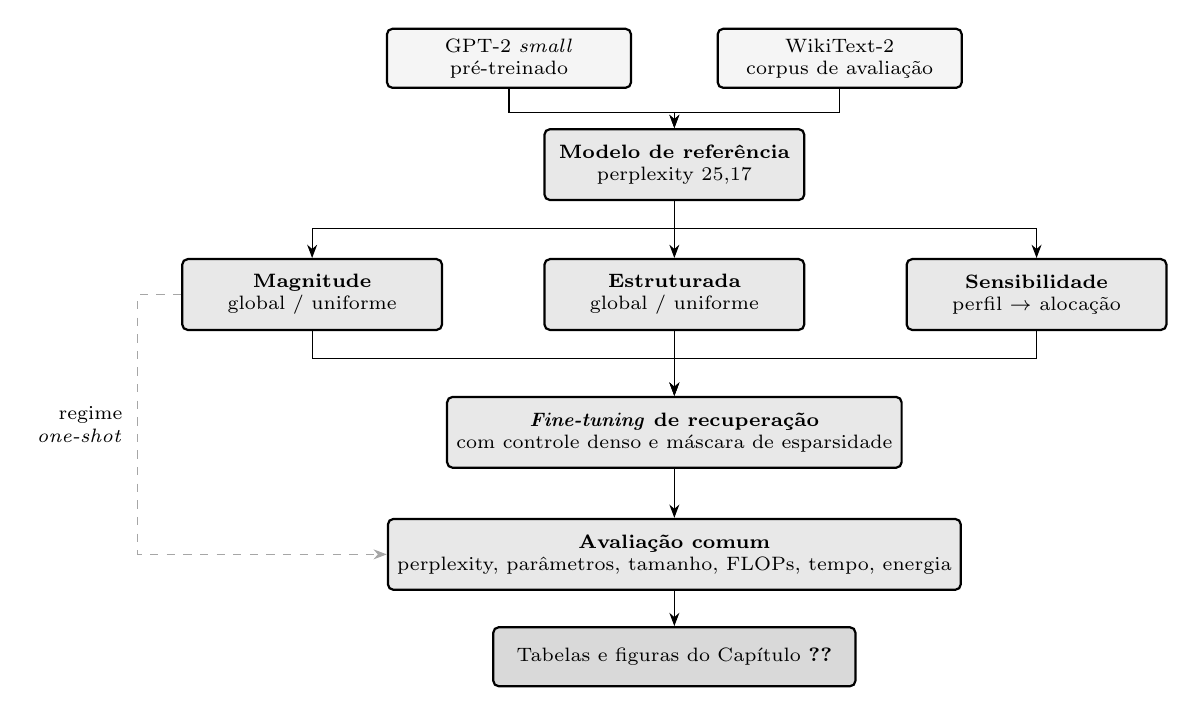
\begin{tikzpicture}[font=\scriptsize, node distance=0.55cm and 0.45cm,
  fonte/.style={rectangle,rounded corners=2pt,draw,thick,fill=gray!8,
                minimum width=3.1cm,minimum height=0.75cm,align=center},
  etapa/.style={rectangle,rounded corners=2pt,draw,thick,fill=gray!18,
                minimum width=3.3cm,minimum height=0.9cm,align=center},
  saida/.style={rectangle,rounded corners=2pt,draw,thick,fill=gray!30,
                minimum width=4.6cm,minimum height=0.75cm,align=center}]

  % --- entradas ---
  \node[fonte] (mod) at (-2.1,0) {GPT-2 \textit{small}\\ \scriptsize pré-treinado};
  \node[fonte] (dat) at (2.1,0) {WikiText-2\\ \scriptsize corpus de avaliação};

  % --- baseline ---
  \node[etapa] (base) at (0,-1.35) {\textbf{Modelo de referência}\\ \scriptsize perplexity 25,17};
  \draw[-{Stealth}] (mod.south) -- ++(0,-0.3) -| (base.north);
  \draw[-{Stealth}] (dat.south) -- ++(0,-0.3) -| (base.north);

  % --- três estratégias ---
  \node[etapa] (mag) at (-4.6,-3.0) {\textbf{Magnitude}\\ \scriptsize global / uniforme};
  \node[etapa] (est) at (0,-3.0)    {\textbf{Estruturada}\\ \scriptsize global / uniforme};
  \node[etapa] (sen) at (4.6,-3.0)  {\textbf{Sensibilidade}\\ \scriptsize perfil $\rightarrow$ alocação};
  \foreach \n in {mag,est,sen} \draw[-{Stealth}] (base.south) -- ++(0,-0.35) -| (\n.north);

  % --- fine-tuning ---
  \node[etapa] (ft) at (0,-4.75) {\textbf{\textit{Fine-tuning} de recuperação}\\
        \scriptsize com controle denso e máscara de esparsidade};
  \foreach \n in {mag,est,sen} \draw[-{Stealth}] (\n.south) -- ++(0,-0.35) -| (ft.north);

  % --- avaliação ---
  \node[etapa] (av) at (0,-6.3) {\textbf{Avaliação comum}\\
        \scriptsize perplexity, parâmetros, tamanho, FLOPs, tempo, energia};
  \draw[-{Stealth}] (ft) -- (av);

  \node[saida] (out) at (0,-7.6) {Tabelas e figuras do Capítulo~\ref{chap:resultados}};
  \draw[-{Stealth}] (av) -- (out);

  % --- desvio one-shot ---
  \draw[-{Stealth},dashed,gray!70] (mag.west) -- ++(-0.55,0)
     |- node[left=2pt,align=right,font=\scriptsize,black,pos=0.25]
        {regime\\ \textit{one-shot}} (av.west);
\end{tikzpicture}
\fonte{Elaborada pelo autor.}
\end{figure}

Como indica a linha tracejada da figura, as varreduras \textit{one-shot} contornam a etapa
de \textit{fine-tuning} e vão direto à avaliação. Essa bifurcação é o que permite separar,
nos resultados, o dano causado pela poda daquilo que o retreinamento consegue recuperar.

\section{Métricas de Avaliação}\label{sec:metricas}

Toda configuração --- o modelo denso, as podadas pelos métodos da literatura e as podadas
pela estratégia otimizada --- é avaliada pelo mesmo conjunto de métricas, cobrindo as três
dimensões definidas na Seção~\ref{sec:metodologia_metricas}. A
Tabela~\ref{tab:metricas} as resume.

\begin{table}[htb]
\centering
\caption{Métricas de avaliação coletadas para cada configuração.}
\label{tab:metricas}
\small
\begin{tabular}{p{3.2cm} p{6.1cm} p{1.7cm} p{2.2cm}}
\hline
\textbf{Métrica} & \textbf{O que mede} & \textbf{Unidade} & \textbf{Ferramenta} \\
\hline
Perplexity & Qualidade da modelagem da linguagem; quanto menor, melhor & --- & PyTorch \\
Parâmetros totais & Parâmetros existentes na arquitetura & unidades & PyTorch \\
Parâmetros não nulos & Parâmetros efetivamente diferentes de zero & unidades & PyTorch \\
Esparsidade real & Fração de parâmetros podáveis eliminados & \% & PyTorch \\
Tamanho do modelo & Memória ocupada pelos parâmetros & MB & PyTorch \\
FLOPs & Operações de ponto flutuante por inferência & FLOPs & \texttt{thop} \\
Tempo de inferência & Tempo médio de uma passagem direta & ms & \texttt{perf\_counter} \\
Energia consumida & Energia gasta durante a avaliação & kWh & \texttt{CodeCarbon} \\
Emissões de $CO_2$ & Emissões equivalentes ao consumo & kg & \texttt{CodeCarbon} \\
\hline
\end{tabular}\\
\textit{Fonte: Elaboração própria.}
\end{table}

\subsection{Perplexity}\label{subsec:metrica_perplexity}

A perplexity é a métrica de desempenho preditivo adotada. Ela é calculada pelo método da
janela deslizante, padrão para modelos autorregressivos: o fluxo de \textit{tokens} do
conjunto de teste é percorrido em janelas do tamanho máximo de contexto do modelo, com
passo menor que a janela, de modo que cada \textit{token} seja previsto dispondo de
contexto anterior substancial. Apenas os \textit{tokens} ainda não avaliados contribuem
para a perda em cada janela; os demais entram como contexto.

Emprega-se janela de 1.024 \textit{tokens} com passo de 512. Passos menores produzem
estimativas mais precisas ao custo de mais computação; o valor adotado é o compromisso
usual na literatura, e é mantido idêntico em todas as configurações avaliadas.

\subsection{Custo Computacional}\label{subsec:metrica_custo}

A contagem de \textbf{parâmetros} é reportada em duas formas complementares. O total
reflete o que existe na arquitetura; a contagem de não nulos reflete o que sobrou depois da
poda. Na poda não estruturada as duas divergem --- há zeros, mas a arquitetura é a mesma
---, enquanto na poda estruturada elas coincidem, pois o que foi removido deixou de
existir. Essa divergência é, por si só, um resultado: ela evidencia a diferença entre
compressão contábil e compressão física.

A \textbf{esparsidade real} reportada nas tabelas é sempre calculada sobre o conjunto
podável, mas a natureza do cálculo acompanha a estratégia: na poda por magnitude é a fração
de pesos anulados nas 48 matrizes; na poda estruturada é a fração de parâmetros que
deixaram de existir nas mesmas projeções, vieses incluídos, já que a remoção de uma
estrutura elimina também o viés que lhe corresponde. As duas grandezas medem a mesma coisa
--- quanto do conjunto podável foi eliminado ---, mas não são idênticas em denominador, e
diferenças na segunda casa decimal entre estratégias não devem ser interpretadas.

Os \textbf{FLOPs} são contabilizados por análise do grafo computacional. Registre-se uma
particularidade da implementação: as projeções internas do GPT-2 não são camadas lineares
convencionais, e sim um tipo específico de camada que a ferramenta de contagem não
reconhece por padrão. Sem tratamento, a contagem ignoraria justamente as matrizes que a
poda modifica, e a métrica sairia constante. Foi necessário, portanto, registrar uma regra
de contagem própria para esse tipo de camada. Reconhece-se uma limitação remanescente: as
multiplicações de matriz internas ao mecanismo de atenção não são contabilizadas pela
ferramenta em nenhuma configuração. Como a omissão é idêntica para todas as estratégias,
as comparações permanecem válidas. A implementação prevê ainda um estimador analítico de
reserva --- duas operações por parâmetro não pertencente aos \textit{embeddings}, por
\textit{token} processado ---, acionado apenas se a contagem pelo grafo falhar. Todos os
valores reportados no Capítulo~\ref{chap:resultados} provêm da contagem pelo grafo, o que
se verifica pelo fato de os FLOPs variarem com a poda estruturada; o estimador de reserva
produziria uma grandeza de natureza diferente e não deve ser misturado a eles.

O \textbf{tempo de inferência} é medido sobre uma entrada representativa de 512
\textit{tokens}, com execuções de aquecimento descartadas --- para mitigar efeitos de
inicialização da GPU --- seguidas de execuções cronometradas, das quais se reporta média e
desvio-padrão.

\subsection{Impacto Ambiental}\label{subsec:metrica_energia}

O consumo de \textbf{energia} é medido com o \texttt{CodeCarbon}, que monitora o
\textit{hardware} durante a execução do bloco de avaliação e reporta a energia consumida em
quilowatts-hora. As \textbf{emissões de $CO_2$} são estimadas a partir desse consumo e da
intensidade de carbono da rede elétrica onde o código executa.

Sobre esta última métrica cabe uma ressalva importante, identificada durante os
experimentos: a intensidade de carbono utilizada varia conforme a sessão de execução. Em
consequência, as emissões não são comparáveis entre execuções realizadas em sessões
distintas, e a análise dos resultados apoia-se no consumo de energia, não nas emissões
derivadas dele.

\section{Ambiente de Execução e Reprodutibilidade}\label{sec:ambiente}

Os experimentos são executados na plataforma Kaggle, em sessões com GPU NVIDIA Tesla T4. A
implementação detecta automaticamente o dispositivo disponível, o que permite executar
localmente em CPU para testes rápidos sem alteração de código.

Quanto à reprodutibilidade, três aspectos merecem registro.

O primeiro é que as varreduras \textit{one-shot} são \textbf{determinísticas}. Não há
treinamento, o modelo opera em modo de avaliação, o conjunto de teste é fixo e os critérios
de poda são ordenações determinísticas sobre pesos fixos. Verificou-se empiricamente que
execuções independentes, em sessões distintas, reproduzem a perplexity até a última casa
decimal. Repetições com sementes diferentes, nessas etapas, produziriam linhas idênticas e
não acrescentariam informação. A semente passa a importar apenas no \textit{fine-tuning}.

O segundo é que as medições de \textbf{tempo e energia dependem da sessão}. Observou-se que
o mesmo modelo denso, sem qualquer poda, registrou tempos e consumos sensivelmente
distintos em sessões diferentes da plataforma, o que se atribui à variação de
\textit{hardware} físico e de carga concorrente. Por essa razão, comparações de custo entre
varreduras executadas em sessões distintas são sempre feitas em termos relativos ao modelo
denso da própria sessão, nunca em valores absolutos.

O terceiro é que cada configuração experimental grava uma linha em arquivo de resultados,
contendo não apenas as métricas mas também os parâmetros que a geraram --- estratégia,
escopo, taxa alvo, taxa efetiva e, no caso da estratégia otimizada, as taxas atribuídas a
cada camada. Isso permite rastrear qualquer número apresentado no
Capítulo~\ref{chap:resultados} até a configuração exata que o produziu.

\section{Limitações Metodológicas}\label{sec:limitacoes}

Reconhecem-se, desde o desenho experimental, limitações que condicionam o escopo dos
resultados:

\begin{itemize}
    \item \textbf{Um único modelo e um único corpus.} Os experimentos empregam
          exclusivamente o GPT-2 \textit{small} sobre o WikiText-2. Os resultados podem
          não se transferir diretamente para modelos de escala substancialmente maior ou
          para corpora de natureza distinta. A implementação foi mantida parametrizável
          justamente para viabilizar essa verificação em trabalhos futuros.

    \item \textbf{Duas estratégias de poda, e não mais.} A restrição de tempo experimental
          levou à escolha de duas estratégias que cobrem os extremos de granularidade.
          Métodos baseados em informação de gradiente ou de segunda ordem ficaram fora do
          escopo.

    \item \textbf{Faixa restrita de taxas-sonda no perfil de sensibilidade.} O perfil que
          alimenta a alocação é levantado a uma única taxa, e sua estabilidade foi
          verificada por meio de uma réplica a uma segunda taxa
          (Seção~\ref{subsec:robustez_sonda}). Ambas pertencem, porém, ao mesmo regime
          intermediário de poda: nada garante que a ordenação de sensibilidade entre
          camadas se mantenha em regimes muito mais brandos ou muito mais agressivos.

    \item \textbf{Sensibilidade medida em isolamento.} A sonda mede o efeito de cada camada
          isoladamente e ignora interações entre elas. Como se verifica no
          Capítulo~\ref{chap:resultados}, a degradação é fortemente superaditiva, de modo
          que o perfil deve ser lido como ordenação relativa de importância, e não como
          modelo preditivo do desempenho de uma configuração completa.

    \item \textbf{Dependência do \textit{hardware}.} Tempo e energia são intrinsecamente
          dependentes da máquina. Os valores absolutos não devem ser comparados entre
          ambientes distintos; a análise apoia-se em comparações relativas dentro de um
          mesmo ambiente.

    \item \textbf{Hiperparâmetros não otimizados exaustivamente.} Os hiperparâmetros do
          \textit{fine-tuning} foram definidos a partir da literatura e de experimentos
          preliminares, sem busca sistemática. Valores melhores podem existir.

    \item \textbf{Semente única no \textit{fine-tuning}.} Esta é a única etapa estocástica
          do experimento, e todas as configurações foram executadas com uma única semente.
          As perplexities pós-retreinamento não vêm, portanto, acompanhadas de estimativa
          de variância, e diferenças pequenas entre configurações retreinadas devem ser
          lidas com a cautela correspondente. A comparação principal da etapa --- alocação
          guiada contra alocação global --- é afetada por essa limitação justamente no
          orçamento em que as duas praticamente empatam.

    \item \textbf{Estimativa de emissões.} A conversão de energia em emissões depende de
          tabelas regionais de intensidade de carbono, que carregam incerteza e variaram
          entre as sessões de execução. As emissões devem ser lidas como aproximações de
          ordem de grandeza.
\end{itemize}

Apesar dessas limitações, o desenho descrito é suficiente para responder às duas perguntas
enunciadas na Seção~\ref{sec:visao_geral}, que são o objeto do
Capítulo~\ref{chap:resultados}.
         % capítulo Desenvolvimento (antigo, renomeado)
\chapter{Resultados}\label{chap:resultados}

Este capítulo apresenta os resultados experimentais obtidos com o GPT-2
\textit{small} sobre o WikiText-2. A exposição segue a ordem em que os
experimentos foram conduzidos: primeiro as duas estratégias clássicas de poda
--- magnitude (Seção~\ref{sec:res_magnitude}) e estruturada
(Seção~\ref{sec:res_estruturada}) ---, cujos resultados delimitam o problema;
em seguida a estratégia otimizada proposta, em suas duas fases: o
levantamento do perfil de sensibilidade por camada
(Seção~\ref{sec:perfil_sensibilidade}) e a varredura da alocação dele
derivada (Seção~\ref{sec:res_alocacao}). A Seção~\ref{sec:res_sintese}
sintetiza os achados.

\section{Protocolo e Modelo de Referência}\label{sec:res_protocolo}

Todos os experimentos partem do GPT-2 \textit{small} pré-treinado
(124.439.808 parâmetros), avaliado no conjunto de teste do WikiText-2 por
janela deslizante com \textit{stride} de 512 \textit{tokens}. A perplexity do
modelo denso é de \textbf{25,17}, valor coerente com o reportado na
literatura para essa configuração, o que valida a implementação do
procedimento de avaliação. As medições de custo do modelo denso são: 474,70~MB
de memória de parâmetros e 126,6~GFLOPs por janela de 512 \textit{tokens}.

Duas ressalvas metodológicas condicionam a leitura das tabelas que se seguem.

A primeira é que \textbf{todos os resultados deste capítulo são
\textit{one-shot}}: poda-se o modelo pré-treinado e mede-se imediatamente, sem
qualquer \textit{fine-tuning} de recuperação. Essa escolha isola o efeito da
poda do efeito do retreinamento, mas implica que as perplexities aqui
reportadas são substancialmente piores que as da literatura, em que a poda é
seguida de retreinamento. As curvas não devem, portanto, ser lidas como
proposta de configuração de uso, e sim como medida do dano que cada estratégia
de alocação causa por si só.

A segunda é que as varreduras foram executadas em sessões distintas do
ambiente Kaggle, e as medições de \textbf{custo dependem da sessão}. O mesmo
modelo denso registrou 40,5~ms por janela em uma sessão, 54,0~ms em outra e
46,3~ms em uma terceira; o consumo de energia do modelo denso variou de
forma análoga, entre 1176 e 1572~$\mu$Wh. Por essa razão, comparações de tempo
e energia \textbf{entre} varreduras são sempre apresentadas em termos
relativos ao \textit{baseline} da própria sessão, nunca em valores absolutos.
As emissões de $\text{CO}_2$, que dependem adicionalmente do fator de carbono
da rede elétrica do \textit{datacenter} --- que também variou entre sessões
---, não são comparadas entre varreduras.

\section{Poda por Magnitude}\label{sec:res_magnitude}

A Tabela~\ref{tab:magnitude} apresenta a varredura da poda por magnitude
\cite{Han2015} nos dois escopos de alocação implementados:
\textit{global}, em que um único limiar sobre o valor absoluto dos pesos é
aplicado a toda a rede, e \textit{uniforme}, em que cada camada recebe a mesma
fração de poda, com limiar próprio.

\begin{table}[htb]
\centering
\caption{Poda por magnitude \textit{one-shot} no GPT-2 \textit{small} /
WikiText-2. As colunas de custo referem-se ao escopo uniforme; o escopo global
produz valores idênticos, pois nenhum dos dois altera a arquitetura.}
\label{tab:magnitude}
\small
\begin{tabular}{c cc ccc}
\toprule
\textbf{Esparsidade} & \multicolumn{2}{c}{\textbf{Perplexity}} & \multicolumn{3}{c}{\textbf{Custo}} \\
\cmidrule(lr){2-3} \cmidrule(lr){4-6}
 & \textbf{Global} & \textbf{Uniforme} & \textbf{Params. $\neq 0$} & \textbf{Tamanho} & \textbf{FLOPs} \\
\midrule
0\,\%  &    25,17 &    25,17 & 124,4\,M & 474,7\,MB & 126,6\,G \\
10\,\% &    25,40 &    25,47 & 115,9\,M & 474,7\,MB & 126,6\,G \\
20\,\% &    26,87 &    27,22 & 107,5\,M & 474,7\,MB & 126,6\,G \\
30\,\% &    40,23 &    36,42 &  99,0\,M & 474,7\,MB & 126,6\,G \\
40\,\% &   165,20 &   104,82 &  90,5\,M & 474,7\,MB & 126,6\,G \\
50\,\% &  1096,50 &   473,28 &  82,0\,M & 474,7\,MB & 126,6\,G \\
60\,\% &  5121,25 &  2004,20 &  73,5\,M & 474,7\,MB & 126,6\,G \\
70\,\% &  9371,16 &  6891,85 &  65,0\,M & 474,7\,MB & 126,6\,G \\
80\,\% &  8847,27 & 10871,00 &  56,5\,M & 474,7\,MB & 126,6\,G \\
90\,\% &  4612,69 & 13996,88 &  48,0\,M & 474,7\,MB & 126,6\,G \\
\bottomrule
\end{tabular}
\end{table}

O resultado mais importante da tabela está nas três últimas colunas, e é
negativo: \textbf{o custo não cai}. Entre 0\,\% e 90\,\% de esparsidade, o
número de parâmetros não nulos cai de 124,4~M para 48,0~M --- uma redução de
61\,\% ---, enquanto o tamanho em memória, os FLOPs e o tempo de inferência
permanecem rigorosamente constantes. A explicação é direta: a poda não
estruturada substitui pesos por zeros, mas não remove nada da arquitetura. Os
tensores mantêm as mesmas dimensões, e a GPU multiplica os zeros exatamente
como multiplicava os valores originais. O ganho de 61\,\% em parâmetros é
contábil, não físico.

Esse achado responde empiricamente, e pela negativa, à primeira das duas
perguntas que orientam este trabalho --- a de se a redução teórica de
parâmetros se converte em redução real de consumo. Na Tesla T4 utilizada, e
sem suporte de \textit{hardware} ou de \textit{kernels} para esparsidade, a
poda não estruturada não entrega ganho de eficiência algum. A pequena
tendência de queda na energia medida (de 1572 para 1432~$\mu$Wh) é da ordem da
variação observada entre execuções repetidas do mesmo modelo denso e não deve
ser interpretada como efeito da poda.

Quanto à qualidade, a curva de perplexity apresenta um joelho acentuado em
torno de 30\,\%. Até 20\,\% de esparsidade a poda é praticamente gratuita
(acréscimo de 0,3 a 2,1 pontos de perplexity); a partir de 40\,\% a
degradação torna-se explosiva. A região utilizável em regime \textit{one-shot}
é, portanto, limitada a esparsidades de até 20\,\%.

Por fim, a comparação entre os dois escopos revela um cruzamento duplo: os
escopos empatam até 20\,\%, o uniforme domina claramente entre 30\,\% e
70\,\% --- exatamente a faixa em que a escolha de alocação teria consequência
prática --- e o global só apresenta valores menores em 80\,\% e 90\,\%, região
em que ambos os modelos já estão destruídos (perplexity acima de 4600) e a
comparação perde sentido. Na faixa que importa, portanto, a alocação uniforme
é preferível à global. Esse é um resultado contraintuitivo: o escopo global é
o que aloca o orçamento com base em uma medida de importância --- a magnitude
do peso --- e ainda assim perde para a alocação que ignora qualquer medida de
importância. Trata-se do primeiro indício de que a magnitude do peso é um
\textit{proxy} pobre para a importância de um parâmetro.

\section{Poda Estruturada}\label{sec:res_estruturada}

A Tabela~\ref{tab:estruturada} apresenta a varredura da poda estruturada
\cite{Li2017}, adaptada ao \textit{Transformer}: remoção física
de cabeças de atenção e de neurônios das camadas MLP, ordenados por norma
$L_1$. A esparsidade-alvo é expressa como fração de \textit{estruturas}
removidas; a fração de parâmetros efetivamente eliminada aparece como
esparsidade real.

\begin{table}[htb]
\centering
\caption{Poda estruturada \textit{one-shot} (cabeças e neurônios MLP,
escopo global) no GPT-2 \textit{small} / WikiText-2. O tempo de inferência é
normalizado pelo \textit{baseline} da mesma sessão (40,5~ms).}
\label{tab:estruturada}
\small
\begin{tabular}{c c ccccc}
\toprule
\textbf{Estrut.} & \textbf{Perplexity} & \textbf{Params.} & \textbf{Tamanho}
& \textbf{FLOPs} & \textbf{Tempo rel.} & \textbf{Energia rel.} \\
\midrule
0\,\%  &   25,17 & 124,4\,M & 474,7\,MB & 126,6\,G & 1,000 & 1,000 \\
10\,\% &  356,20 & 116,0\,M & 442,6\,MB & 118,0\,G & 0,968 & 0,975 \\
20\,\% & 2102,06 & 107,6\,M & 410,5\,MB & 109,3\,G & 0,908 & 0,945 \\
30\,\% & 2413,52 &  99,0\,M & 377,6\,MB & 100,5\,G & 0,831 & 0,865 \\
40\,\% & 2434,92 &  90,6\,M & 345,5\,MB &  91,9\,G & 0,756 & 0,786 \\
50\,\% & 2402,58 &  81,9\,M & 312,6\,MB &  83,1\,G & 0,688 & 0,714 \\
60\,\% & 2957,26 &  73,5\,M & 280,5\,MB &  74,5\,G & 0,628 & 0,638 \\
70\,\% & 4635,36 &  65,1\,M & 248,3\,MB &  65,9\,G & 0,557 & 0,558 \\
80\,\% & 7620,02 &  56,5\,M & 215,5\,MB &  57,0\,G & 0,503 & 0,489 \\
90\,\% & 5822,89 &  48,1\,M & 183,3\,MB &  48,4\,G & 0,445 & 0,413 \\
\bottomrule
\end{tabular}
\end{table}

O contraste com a Tabela~\ref{tab:magnitude} é o achado central deste
trabalho no plano da eficiência. Aqui \textbf{o custo cai, e cai
proporcionalmente aos parâmetros}: a 90\,\% de estruturas removidas, o tempo
de inferência cai 56\,\%, a energia 59\,\%, o tamanho em memória 61\,\% e os
FLOPs 62\,\%, acompanhando a redução de 61\,\% no número de parâmetros. As
duas tabelas formam, juntas, a resposta completa à primeira pergunta
empírica: a redução de parâmetros só se converte em redução de consumo quando
a poda remove estruturas inteiras da arquitetura, e não quando apenas as
zera.

O preço dessa eficiência, contudo, é severo em regime \textit{one-shot}. Já
com 10\,\% de estruturas removidas a perplexity salta de 25,17 para 356,20 ---
compare-se com 25,40 na poda por magnitude ao mesmo nível. \textbf{Não existe
região gratuita} na poda estruturada sem retreinamento, o que é coerente com o
procedimento original de \citeonline{Li2017}, em que a poda é sempre
seguida de \textit{fine-tuning}.

Dois resultados secundários merecem registro. O primeiro é que a inversão de
escopo observada na magnitude se repete ao contrário: na poda estruturada é o
escopo \textbf{global} que domina, e a alocação uniforme colapsa em taxas
altas (perplexity de 53.313 a 80\,\% e de 827.316 a 90\,\%, contra 7620 e 5823
do global). Somado ao achado da seção anterior, isso estabelece que
\textbf{nenhuma das duas alocações ingênuas vence nos dois regimes} --- a
constatação que motiva diretamente a estratégia otimizada.

O segundo é a assimetria entre os dois tipos de estrutura. Remover cabeças de
atenção é notavelmente mais tolerável que remover neurônios MLP: com 129 das
144 cabeças removidas (90\,\%), a perplexity fica em 781, ao passo que a
remoção equivalente de neurônios MLP produz valores acima de 3900. A curva das
cabeças é, ainda, não monotônica, com mínimo local em torno de 30\,\%
(perplexity 162, inferior aos 237 obtidos com apenas 10\,\% removidas) --- eco
direto do achado de \citeonline{Michel2019} sobre a redundância das
cabeças de atenção. Em contrapartida, as camadas MLP concentram cerca de dois
terços dos parâmetros podáveis, de modo que a poda restrita a cabeças tem
alcance limitado como estratégia de compressão.

\section{Perfil de Sensibilidade por Camada}\label{sec:perfil_sensibilidade}

As duas seções anteriores mostraram que nenhuma alocação ingênua do orçamento
de poda domina o espectro de esparsidade: na poda por magnitude o escopo
uniforme prevaleceu na faixa útil (Seção~\ref{sec:res_magnitude}), enquanto na
poda estruturada foi o escopo global que obteve as melhores perplexidades
(Seção~\ref{sec:res_estruturada}) --- e ambas as alocações colapsam em algum
regime. A hipótese central deste trabalho é que a
causa é comum aos dois casos: as camadas do \textit{Transformer} não são
igualmente importantes, de modo que tanto tratá-las de forma idêntica
(alocação uniforme) quanto confiar exclusivamente na magnitude dos pesos como
proxy de importância (alocação global) distribuem mal o orçamento disponível.

Esta seção reporta o experimento que testa diretamente essa hipótese. Para
cada uma das 12 camadas do GPT-2 \textit{small} e para cada uma das duas
estratégias, poda-se \textbf{apenas} aquela camada a uma taxa-sonda fixa de
50\,\%, mantendo-se as demais intactas, e mede-se a perplexity resultante no
conjunto de teste do WikiText-2. Não há \textit{fine-tuning} --- o
procedimento é \textit{one-shot}, como nas varreduras anteriores. A
degradação é registrada em escala logarítmica,

\begin{equation}\label{eq:delta_log_ppl}
\Delta_{\ell} = \ln\!\left(\frac{\text{PPL}_{\ell}}{\text{PPL}_{\text{base}}}\right),
\end{equation}

\noindent onde $\text{PPL}_{\ell}$ é a perplexity do modelo com apenas a
camada $\ell$ podada e $\text{PPL}_{\text{base}} = 25{,}17$ é a perplexity do
modelo denso. O logaritmo é necessário porque a perplexity de modelos podados
sem recuperação varia por ordens de grandeza: em escala linear, uma única
camada catastrófica tornaria as demais indistinguíveis entre si. O
experimento totaliza 24 medições (12 camadas $\times$ 2 estratégias).

\subsection{Perfil Obtido}\label{subsec:perfil_obtido}

A Tabela~\ref{tab:perfil_sensibilidade} apresenta os resultados e a
Figura~\ref{fig:perfil_sensibilidade} os representa graficamente.

\begin{table}[htb]
\centering
\caption{Perfil de sensibilidade por camada do GPT-2 \textit{small} no
WikiText-2. Cada linha corresponde a podar exclusivamente a camada indicada, à
taxa-sonda de 50\,\%, sem \textit{fine-tuning}. Perplexity do modelo denso:
25,17.}
\label{tab:perfil_sensibilidade}
\small
\begin{tabular}{c cc cc}
\toprule
& \multicolumn{2}{c}{\textbf{Poda por magnitude}} & \multicolumn{2}{c}{\textbf{Poda estruturada}} \\
\cmidrule(lr){2-3} \cmidrule(lr){4-5}
\textbf{Camada} & \textbf{Perplexity} & $\boldsymbol{\Delta_{\ell}}$
                & \textbf{Perplexity} & $\boldsymbol{\Delta_{\ell}}$ \\
\midrule
0  & 37,17 & 0,390 & 1386,43 & 4,009 \\
1  & 26,06 & 0,035 &   27,66 & 0,094 \\
2  & 27,62 & 0,093 &   29,91 & 0,173 \\
3  & 26,28 & 0,043 &   30,23 & 0,183 \\
4  & 30,81 & 0,202 &   31,31 & 0,218 \\
5  & 28,66 & 0,130 &   29,80 & 0,169 \\
6  & 27,09 & 0,074 &   28,90 & 0,138 \\
7  & 26,44 & 0,049 &   28,31 & 0,118 \\
8  & 26,59 & 0,055 &   28,45 & 0,122 \\
9  & 26,76 & 0,061 &   27,63 & 0,093 \\
10 & 26,55 & 0,054 &   28,89 & 0,138 \\
11 & 26,55 & 0,054 &   48,87 & 0,663 \\
\midrule
\textbf{Razão máx./mín.} & \multicolumn{2}{c}{11,3$\times$} & \multicolumn{2}{c}{42,9$\times$} \\
\bottomrule
\end{tabular}
\end{table}

\begin{figure}[htb]
\centering
\caption{Degradação $\Delta_{\ell}$ causada pela poda isolada de cada camada,
à taxa-sonda de 50\,\%. Note-se que as escalas verticais diferem entre os dois
gráficos; na poda estruturada, a barra da camada 0 excede o eixo e está
truncada.}
\label{fig:perfil_sensibilidade}
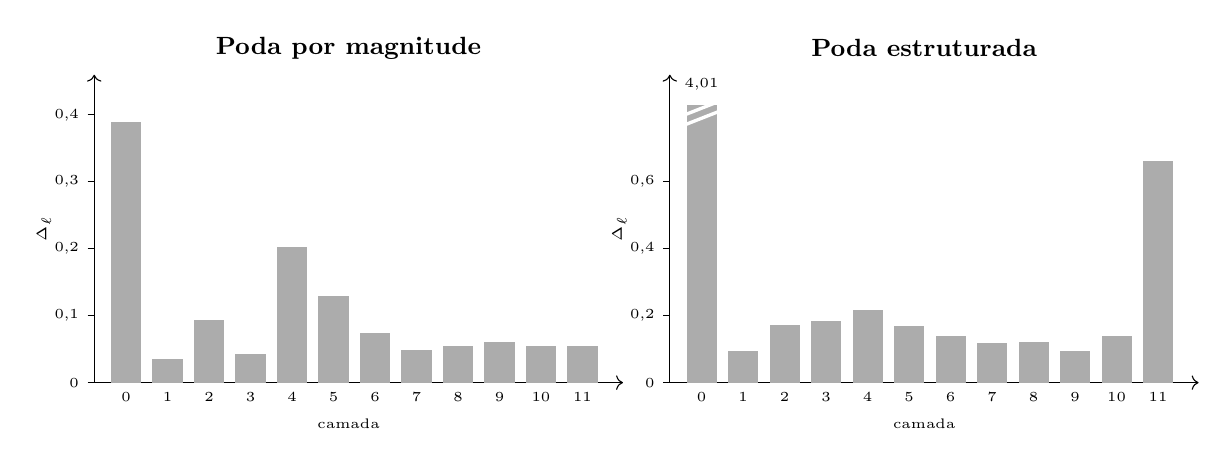
\begin{tikzpicture}[scale=0.85]

  % ---------- painel esquerdo: magnitude ----------
  \begin{scope}
    \draw[->] (-0.2,0) -- (7.7,0);
    \draw[->] (-0.2,0) -- (-0.2,4.6);
    \foreach \y/\lab in {0/0, 1/0{,}1, 2/0{,}2, 3/0{,}3, 4/0{,}4}
      \draw (-0.3,\y*1.0) -- (-0.2,\y*1.0) node[left,xshift=-2pt,font=\tiny] {\lab};
    \foreach \c/\d in {0/0.390, 1/0.035, 2/0.093, 3/0.043, 4/0.202, 5/0.130,
                       6/0.074, 7/0.049, 8/0.055, 9/0.061, 10/0.054, 11/0.054} {
      \fill[gray!65] ({\c*0.62+0.05},0) rectangle ++(0.45,{\d*10});
      \node[font=\tiny] at ({\c*0.62+0.275},-0.22) {\c};
    }
    \node[font=\small\bfseries] at (3.6,5.0) {Poda por magnitude};
    \node[font=\tiny] at (3.6,-0.62) {camada};
    \node[rotate=90,font=\tiny] at (-0.95,2.3) {$\Delta_{\ell}$};
  \end{scope}

  % ---------- painel direito: estruturada ----------
  \begin{scope}[xshift=8.6cm]
    \draw[->] (-0.2,0) -- (7.7,0);
    \draw[->] (-0.2,0) -- (-0.2,4.6);
    \foreach \y/\lab in {0/0, 1/0{,}2, 2/0{,}4, 3/0{,}6}
      \draw (-0.3,\y*1.0) -- (-0.2,\y*1.0) node[left,xshift=-2pt,font=\tiny] {\lab};
    \foreach \c/\d in {1/0.094, 2/0.173, 3/0.183, 4/0.218, 5/0.169,
                       6/0.138, 7/0.118, 8/0.122, 9/0.093, 10/0.138, 11/0.663} {
      \fill[gray!65] ({\c*0.62+0.05},0) rectangle ++(0.45,{\d*5});
      \node[font=\tiny] at ({\c*0.62+0.275},-0.22) {\c};
    }
    % camada 0: barra truncada
    \fill[gray!65] (0.05,0) rectangle (0.50,4.15);
    \draw[white,line width=1.2pt] (0.02,4.0) -- (0.53,4.2);
    \draw[white,line width=1.2pt] (0.02,3.85) -- (0.53,4.05);
    \node[font=\tiny] at (0.275,4.45) {4,01};
    \node[font=\tiny] at (0.275,-0.22) {0};
    \node[font=\small\bfseries] at (3.6,5.0) {Poda estruturada};
    \node[font=\tiny] at (3.6,-0.62) {camada};
    \node[rotate=90,font=\tiny] at (-0.95,2.3) {$\Delta_{\ell}$};
  \end{scope}

\end{tikzpicture}
\fonte{Elaborada pelo autor.}
\end{figure}

O primeiro resultado é que a hipótese se confirma de forma inequívoca: a
sensibilidade está longe de ser uniforme. Sob poda por magnitude, a camada
mais frágil degrada o modelo 11,3 vezes mais que a mais robusta; sob poda
estruturada, 42,9 vezes mais. Tratar as 12 camadas como intercambiáveis ---
que é exatamente o que a alocação uniforme faz --- ignora uma diferença de uma
ordem de grandeza no custo de podar cada uma delas.

\subsection{A Camada 0 como Gargalo}\label{subsec:camada_zero}

O segundo resultado é a magnitude do papel da primeira camada. Nas duas
estratégias ela é a mais sensível, mas o efeito é qualitativamente distinto no
caso estruturado: remover metade das cabeças de atenção e dos neurônios MLP
\textbf{apenas do bloco 0} eleva a perplexity de 25,17 para 1386,43, ou seja,
55 vezes o valor do modelo denso. Para dimensionar esse número, a varredura
estruturada uniforme a 50\,\% --- que poda \textit{todas} as 12 camadas ---
atinge perplexity 4573,00. Em escala logarítmica, a camada 0 sozinha responde
por $4{,}01/5{,}20 \approx 77\,\%$ de toda a degradação produzida pela poda
uniforme do modelo inteiro.

A interpretação é coerente com o papel funcional do primeiro bloco. É nele que
as representações deixam de ser a soma direta de \textit{embeddings} de token
e de posição e passam a ser contextualizadas pela primeira vez; qualquer
informação descartada ali não tem como ser recuperada pelas camadas
subsequentes, que operam sobre um sinal já degradado. Trata-se, portanto, de
um erro que se propaga por toda a pilha, ao contrário de um erro cometido nas
camadas intermediárias.

Na poda estruturada observa-se ainda um segundo ponto crítico na outra
extremidade: a camada 11, imediatamente anterior à cabeça de linguagem,
apresenta $\Delta_{11} = 0{,}663$, quase cinco vezes a mediana das camadas
intermediárias. O perfil estruturado tem, assim, formato aproximado de ``U'':
as bordas da pilha são críticas e o miolo é comparativamente barato. Esse
padrão não se repete na poda por magnitude, cujo perfil decai após um pico
inicial e mantém as últimas camadas entre as mais robustas.

\subsection{Os Perfis Dependem da Estratégia}\label{subsec:perfis_divergem}

O terceiro resultado tem consequência metodológica direta: os dois perfis
\textbf{não} são o mesmo. A correlação de postos de Spearman entre eles é
$\rho = 0{,}50$ --- há concordância, mas parcial. As duas estratégias
coincidem em eleger a camada 0 como a mais crítica e em considerar as camadas
1 e 9 entre as mais robustas, e divergem em praticamente todo o resto: a
camada 11 é a segunda mais sensível sob poda estruturada e apenas a oitava sob
poda por magnitude; a camada 3 é a segunda mais robusta sob magnitude e a
quarta mais sensível sob poda estruturada.

A implicação prática é que não existe um perfil de sensibilidade único do
GPT-2. Sensibilidade é uma propriedade do par (camada, estratégia de poda),
não da camada isoladamente, e o perfil precisa ser levantado separadamente
para cada estratégia --- como foi feito aqui --- sob pena de se alocar o
orçamento com um mapa que pertence a outro método. Esse achado também oferece
uma explicação para a inversão observada nas varreduras ingênuas: como
magnitude de peso e norma de estrutura respondem a aspectos diferentes da
importância de uma camada, é esperado que o escopo global (que decide com base
nessas grandezas) acerte em um caso e erre no outro.

\subsection{Da Sensibilidade à Alocação}\label{subsec:alocacao}

O perfil é um diagnóstico; para virar estratégia, precisa ser convertido em
uma taxa de poda por camada. A regra adotada atribui a cada camada uma taxa
proporcional à sua robustez --- o inverso da degradação medida ---, elevada a
um expoente $\beta$ e escalada por um fator único $\alpha$ tal que a média das
taxas, ponderada pelo número de parâmetros de cada camada, iguale o orçamento
global $s$ pretendido:

\begin{equation}\label{eq:alocacao}
r_{\ell} = \min\!\left(\alpha \cdot \Delta_{\ell}^{-\beta},\ r_{\max}\right),
\qquad
\frac{\sum_{\ell} w_{\ell}\, r_{\ell}}{\sum_{\ell} w_{\ell}} = s,
\end{equation}

\noindent com $w_{\ell}$ o número de parâmetros podáveis da camada $\ell$ e
$r_{\max} = 0{,}95$ um teto que impede que mesmo a camada mais robusta seja
integralmente zerada. O fator $\alpha$ é obtido por bisseção, uma vez que a
fração podada é monótona em $\alpha$. O expoente $\beta$ controla o quanto o
perfil é levado a sério: com $\beta = 0$ a regra degenera na poda uniforme e
com $\beta = 1$ usa-se o inverso puro da degradação; valores intermediários
amortecem a razão entre camadas, o que importa porque essa razão é ilimitada
--- uma camada com $\Delta_{\ell}$ muito próximo de zero receberia
praticamente todo o orçamento.

A Tabela~\ref{tab:alocacao_50} mostra as taxas que a
Equação~\ref{eq:alocacao} produziu para um orçamento global de 50\,\% com
$\beta = 1$. O contraste com a alocação uniforme é acentuado: sob poda
estruturada, a camada 0 recebe 2\,\% de poda e a camada 1 recebe 84\,\%,
enquanto a alocação uniforme aplicaria 50\,\% a ambas.

\begin{table}[htb]
\centering
\caption{Taxas de poda por camada efetivamente aplicadas pela
Equação~\ref{eq:alocacao} para orçamento global de 50\,\% e $\beta = 1$
(coluna \texttt{taxas\_por\_camada} dos registros experimentais). A alocação
uniforme corresponderia a 50\,\% em todas as camadas.}
\label{tab:alocacao_50}
\small
\begin{tabular}{l cccccccccccc}
\toprule
\textbf{Camada} & 0 & 1 & 2 & 3 & 4 & 5 & 6 & 7 & 8 & 9 & 10 & 11 \\
\midrule
Magnitude (\%)   &  8 & 94 & 35 & 75 & 16 & 25 & 44 & 67 & 59 & 53 & 61 & 61 \\
Estruturada (\%) &  2 & 84 & 46 & 43 & 36 & 47 & 57 & 67 & 64 & 85 & 57 & 12 \\
\bottomrule
\end{tabular}
\end{table}

\subsection{Limitações do Perfilamento}\label{subsec:limitacoes_perfil}

Três limitações do procedimento devem ser explicitadas, pois condicionam a
leitura dos resultados da varredura otimizada.

A primeira é que a sonda foi aplicada a uma única taxa (50\,\%). O perfil
mede, portanto, a sensibilidade das camadas naquele regime específico, e nada
garante que a ordenação se mantenha em taxas muito menores ou muito maiores.
A escolha por uma única sonda é uma concessão a custo: cada ponto do perfil
exige uma avaliação completa de perplexity, e o levantamento com múltiplas
sondas multiplicaria proporcionalmente o custo da fase.

A segunda, e mais relevante, é que a sonda mede o efeito de cada camada
\textbf{isoladamente}, ignorando as interações entre elas. Os dados do próprio
experimento mostram que essa aproximação é imperfeita: a soma dos
$\Delta_{\ell}$ individuais sob poda por magnitude é 1,238, ao passo que a
poda uniforme simultânea de todas as camadas a 50\,\% produz degradação
logarítmica de 2,934 --- mais que o dobro. A degradação é fortemente
superaditiva, isto é, os erros introduzidos em camadas distintas se compõem em
vez de simplesmente se somarem. O perfil deve, por isso, ser lido como uma
ordenação relativa de importância, e não como um modelo preditivo da
degradação de uma configuração completa.

A terceira é que todas as medições são \textit{one-shot}, sem
\textit{fine-tuning} de recuperação. Camadas que parecem frágeis nesse regime
poderiam ser recuperáveis com retreinamento, o que eventualmente alteraria a
alocação ótima. A opção pelo regime \textit{one-shot} é deliberada e coerente
com o objetivo do trabalho --- isolar o efeito da poda do efeito do
retreinamento ---, mas restringe a generalidade das conclusões.

Nenhuma dessas limitações invalida o achado principal desta seção, que é
robusto às três: sob qualquer leitura, as camadas do GPT-2 diferem entre si
por mais de uma ordem de grandeza no custo de serem podadas, e essa diferença
é informação que as alocações uniforme e global simplesmente não utilizam. Se
essa informação se converte em ganho efetivo na fronteira entre compressão e
qualidade é o que a varredura da estratégia otimizada, reportada na seção
seguinte, se propõe a verificar.

\section{Varredura da Alocação Guiada por Sensibilidade}\label{sec:res_alocacao}

Esta seção reporta a fase que responde à pergunta central do trabalho: a
alocação derivada do perfil de sensibilidade melhora, de fato, o compromisso
entre compressão e qualidade em relação às alocações ingênuas? As taxas por
camada produzidas pela Equação~\ref{eq:alocacao} foram aplicadas nos mesmos
nove níveis de orçamento das varreduras anteriores, para as duas estratégias, e
avaliadas com o mesmo vetor de métricas. O experimento foi replicado com dois
valores do expoente $\beta$ --- 1,0 e 0,5 ---, o que fornece a ablação da
função de alocação sobre um mesmo perfil.

\subsection{Poda por Magnitude}\label{subsec:aloc_magnitude}

A Tabela~\ref{tab:comp_magnitude} compara as quatro alocações.

\begin{table}[htb]
\centering
\caption{Perplexity da poda por magnitude sob as quatro alocações. Em negrito,
o menor valor de cada linha.}
\label{tab:comp_magnitude}
\small
\begin{tabular}{c cc cc}
\toprule
& \multicolumn{2}{c}{\textbf{Alocação ingênua}} & \multicolumn{2}{c}{\textbf{Guiada por sensibilidade}} \\
\cmidrule(lr){2-3} \cmidrule(lr){4-5}
\textbf{Esparsidade} & \textbf{Global} & \textbf{Uniforme} & $\boldsymbol{\beta = 1{,}0}$ & $\boldsymbol{\beta = 0{,}5}$ \\
\midrule
10\,\% & \textbf{25,40} &    25,47 &    25,44 &    25,44 \\
20\,\% &    26,87 &    27,22 &    26,79 & \textbf{26,57} \\
30\,\% &    40,23 &    36,42 &    34,62 & \textbf{31,20} \\
40\,\% &   165,20 &   104,82 &   193,83 & \textbf{57,30} \\
50\,\% &  1096,50 &   473,28 &  1026,09 & \textbf{447,57} \\
60\,\% &  5121,25 &  2004,20 & \textbf{1524,55} &  2171,79 \\
70\,\% &  9371,16 &  6891,85 & \textbf{1853,30} &  2805,39 \\
80\,\% &  8847,27 & 10871,00 & \textbf{2747,56} &  3715,68 \\
90\,\% & \textbf{4612,69} & 13996,88 & 10398,10 &  7616,63 \\
\bottomrule
\end{tabular}
\end{table}

A alocação guiada vence em oito dos nove níveis, e as margens são
substanciais na faixa de interesse. Em 30\,\% de esparsidade, a perplexity cai
de 36,42 (melhor alocação ingênua) para 31,20 --- uma redução de 14\,\%. Em
40\,\%, o ganho é de 104,82 para 57,30, ou seja, a degradação é praticamente
\textbf{reduzida à metade} usando exatamente o mesmo orçamento de poda. Em
50\,\% a vantagem persiste, ainda que modesta (447,57 contra 473,28). Nos
níveis altos, de 60\,\% a 80\,\%, a configuração com $\beta = 1$ produz
perplexities entre 2,5 e 4 vezes menores que a melhor alocação ingênua ---
embora, nesse regime, todos os modelos já estejam degradados a ponto de a
comparação ter interesse mais teórico que prático.

A única derrota ocorre em 90\,\%, onde o escopo global apresenta o menor valor.
Como discutido na Seção~\ref{sec:res_magnitude}, essa é a região em que a
perplexity de todas as configurações ultrapassa 4600 e a ordenação entre
modelos igualmente inservíveis não carrega significado.

\subsection{Poda Estruturada}\label{subsec:aloc_estruturada}

Na poda estruturada, os ganhos são de outra ordem de grandeza, como mostra a
Tabela~\ref{tab:comp_estruturada}.

\begin{table}[htb]
\centering
\caption{Perplexity da poda estruturada sob as quatro alocações. Em negrito, o
menor valor de cada linha.}
\label{tab:comp_estruturada}
\small
\begin{tabular}{c cc cc}
\toprule
& \multicolumn{2}{c}{\textbf{Alocação ingênua}} & \multicolumn{2}{c}{\textbf{Guiada por sensibilidade}} \\
\cmidrule(lr){2-3} \cmidrule(lr){4-5}
\textbf{Estruturas} & \textbf{Global} & \textbf{Uniforme} & $\boldsymbol{\beta = 1{,}0}$ & $\boldsymbol{\beta = 0{,}5}$ \\
\midrule
10\,\% &   356,20 &    481,13 & \textbf{124,29} &    215,83 \\
20\,\% &  2102,06 &   1484,89 & \textbf{371,07} &    717,19 \\
30\,\% &  2413,52 &   5467,56 & \textbf{724,53} &    923,65 \\
40\,\% &  2434,92 &  10486,71 & \textbf{1301,15} &   9489,87 \\
50\,\% &  2402,58 &   4573,00 & \textbf{2327,59} &   7922,81 \\
60\,\% & \textbf{2957,26} &   5799,76 &  5393,15 &  12322,05 \\
70\,\% & \textbf{4635,36} &  12249,58 & 10130,33 & 103463,60 \\
80\,\% & \textbf{7620,02} &  53313,38 &  8891,77 & 203995,84 \\
90\,\% &  5822,89 & 827316,19 &  5353,85 & \textbf{4830,24} \\
\bottomrule
\end{tabular}
\end{table}

Na faixa de 10\,\% a 50\,\% de estruturas removidas, a alocação guiada com
$\beta = 1$ domina de forma inequívoca. Em 10\,\%, a perplexity cai de 356,20
para 124,29 --- uma redução de 65\,\%. Em 20\,\%, de 1484,89 para 371,07, um
fator de \textbf{quatro}. Em 30\,\%, de 2413,52 para 724,53, um fator de
\textbf{3,3}. Considerando que a Seção~\ref{sec:res_estruturada} concluiu que
não existe região gratuita para a poda estruturada \textit{one-shot}, reduzir a
perplexity a um quarto no mesmo orçamento é o resultado mais expressivo deste
capítulo.

Uma ressalva quantitativa é necessária. Como a remoção de estruturas é
discreta, as taxas fracionárias por camada não são atingíveis exatamente, e a
alocação guiada acaba removendo uma fração de parâmetros ligeiramente menor que
a ingênua no mesmo alvo: em 10\,\%, esparsidade real de 9,20\,\% contra
9,90\,\% do escopo global; em 30\,\%, 29,01\,\% contra 29,95\,\%. Parte da
vantagem observada deve-se, portanto, a um corte marginalmente menor. A
diferença é de menos de um ponto percentual de esparsidade, ao passo que a
diferença de perplexity chega a um fator de quatro, de modo que a explicação
não se sustenta como causa principal --- mas o efeito existe e deve ser
declarado.

A partir de 60\,\%, a ordenação se inverte e o escopo global volta a vencer. A
causa é identificável nas taxas alocadas: a partir desse orçamento, um número
crescente de camadas satura no teto $r_{\max} = 0{,}95$ --- duas camadas em
60\,\%, quatro em 70\,\%, oito em 80\,\% e onze em 90\,\%. Saturadas as
camadas, a alocação deixa de discriminar entre elas e degenera em algo próximo
da poda uniforme sobre o subconjunto saturado, ao mesmo tempo em que concentra
uma pressão crescente sobre as poucas camadas ainda livres. A estratégia
guiada, portanto, \textbf{só é informativa enquanto o orçamento couber dentro
do teto por camada}; acima disso, ela perde sua vantagem estrutural. Esse é um
limite intrínseco de qualquer alocação proporcional com teto, e não um defeito
de implementação.

\subsection{Ablação do Expoente $\beta$}\label{subsec:ablacao_beta}

A comparação entre $\beta = 1{,}0$ e $\beta = 0{,}5$ produz um resultado que
não era antecipado: \textbf{o valor adequado de $\beta$ depende da
estratégia}, e depende dela de forma oposta nas duas.

Na poda estruturada, $\beta = 1$ domina em todos os níveis até 80\,\%, e o
amortecimento é francamente prejudicial --- em 70\,\% e 80\,\% a configuração
com $\beta = 0{,}5$ produz perplexities de 103.463 e 203.996, uma ordem de
grandeza pior que qualquer outra alocação testada. Na poda por magnitude ocorre
o inverso na faixa útil: $\beta = 0{,}5$ é melhor de 20\,\% a 50\,\%, e só a
partir de 60\,\% o expoente pleno passa à frente.

A explicação mais plausível liga-se à dispersão dos perfis. O perfil
estruturado tem razão máximo/mínimo de 42,9$\times$ e é dominado pela camada 0,
cuja fragilidade é tão extrema (Seção~\ref{subsec:camada_zero}) que qualquer
amortecimento da alocação lhe devolve orçamento de poda com consequências
catastróficas: em 70\,\%, $\beta = 0{,}5$ atribui 14,6\,\% de poda à camada 0,
contra 3,0\,\% de $\beta = 1$. Quando o perfil contém um sinal dessa
intensidade, convém segui-lo integralmente. Já o perfil de magnitude tem
dispersão de 11,3$\times$, distribuída entre várias camadas de sensibilidade
intermediária; nele, a razão entre camadas é mais suscetível a ruído de
medição, e amortecê-la funciona como regularização. O expoente $\beta$
comporta-se, assim, como um parâmetro de confiança no perfil: quanto mais
nítido o sinal, maior o $\beta$ que compensa adotar.

\subsection{Efeito sobre o Custo}\label{subsec:aloc_custo}

Do ponto de vista da eficiência, a alocação guiada preserva integralmente o
comportamento da estratégia de base, o que era esperado, uma vez que ela
altera a distribuição do orçamento, não sua natureza. Na poda por magnitude,
tamanho, FLOPs e tempo permanecem constantes, pelo mesmo motivo discutido na
Seção~\ref{sec:res_magnitude}. Na poda estruturada, o custo cai
proporcionalmente: normalizando pelo \textit{baseline} da própria sessão, a
configuração com $\beta = 1$ registra tempo relativo de 0,659 e energia
relativa de 0,674 em 50\,\%, e 0,419 e 0,384 em 90\,\% --- valores
equivalentes, dentro da variação entre sessões, aos 0,688 e 0,714 (50\,\%) e
0,445 e 0,413 (90\,\%) do escopo global.

O achado prático é, portanto, que \textbf{o ganho de qualidade da alocação
guiada é gratuito em termos de custo}: na faixa de 10\,\% a 50\,\% da poda
estruturada, obtém-se uma perplexity de três a quatro vezes menor com
essencialmente o mesmo tempo de inferência, o mesmo consumo de energia e o
mesmo tamanho de modelo. É exatamente o deslocamento da fronteira entre
compressão e qualidade que a segunda pergunta empírica do trabalho se propunha
a investigar.

\section{Síntese dos Resultados}\label{sec:res_sintese}

Os experimentos permitem responder às duas perguntas que orientaram o
trabalho.

À primeira --- se a redução teórica de parâmetros se converte em redução real
de consumo --- a resposta é condicional à granularidade da poda. A poda não
estruturada por magnitude reduz em 61\,\% os parâmetros não nulos sem
alterar em nada o tempo de inferência, a energia, o tamanho em memória ou os
FLOPs: na Tesla T4 utilizada, sem suporte de \textit{hardware} para
esparsidade, o ganho é puramente contábil. A poda estruturada, ao remover
fisicamente cabeças de atenção e neurônios MLP, converte a mesma redução de
61\,\% em parâmetros em quedas de 56\,\% no tempo, 59\,\% na energia e 62\,\%
nos FLOPs. Para o objetivo declarado deste trabalho --- redução do consumo de
energia ---, apenas a poda estruturada é uma estratégia viável.

À segunda --- se a alocação otimizada empurra a fronteira entre compressão e
qualidade --- a resposta é afirmativa, com escopo delimitado. As camadas do
GPT-2 diferem entre si por mais de uma ordem de grandeza no custo de serem
podadas, com a camada 0 respondendo isoladamente por cerca de três quartos da
degradação da poda uniforme; essa informação, que nenhuma alocação ingênua
utiliza, converte-se em ganho mensurável quando incorporada à distribuição do
orçamento. Na poda estruturada --- a estratégia que efetivamente reduz consumo
--- a alocação guiada reduz a perplexity por fatores de três a quatro na faixa
de 10\,\% a 50\,\% de estruturas removidas, sem custo adicional de tempo,
energia ou memória. O escopo da conclusão é delimitado por três fronteiras: o
regime \textit{one-shot}, a saturação da alocação em orçamentos acima de
60\,\%, e o fato de que o perfil de sensibilidade precisa ser levantado
separadamente para cada estratégia de poda, por não ser transferível entre
elas.

\include{06_capitulo/consideracoes}


\bookmarksetup{startatroot}% 
% ---

\postextual


\bibliography{referencias}
%\bibliographystyle{abnt-num}
%\bibliographystyle{plainnat}

\chapter{Apêndice}

\begin{apendicesenv}

[TO DO]

\end{apendicesenv}

\begin{comment}
%\glossary
%\begin{anexosenv}
%\end{anexosenv}
%\printindex
\end{comment}

\end{document}
